\documentclass[a4j,12pt]{jreport}
%\documentclass{jreport}
\usepackage[dvipdfmx]{graphicx}
% \usepackage[dvipdfmx]{graphics}
\usepackage{amsmath,amssymb}
% \usepackage{amsmath}
%\usepackage{pxjahyper}
\usepackage{here}
\usepackage{algorithm}
\usepackage{algorithmic}
%\usepackage{algpseudocode}
\usepackage{hhline} 
\usepackage[hang,small,bf]{caption}
\usepackage[subrefformat=parens]{subcaption}
\usepackage{url}
\usepackage{bm}
\captionsetup{compatibility=false}
 
 %pTeX(ptex2pdf)

\def\syaji{ \chapter*{謝辞} \addcontentsline{toc}{chapter}{謝辞}}
\renewcommand{\bibname}{参考文献}
\setlength{\textheight}{\paperheight}
\setlength{\topmargin}{4.6mm}
\addtolength{\topmargin}{-\headheight}
\addtolength{\topmargin}{-\headsep}
\addtolength{\topmargin}{-\headheight}
\addtolength{\textheight}{-60mm}

\setlength{\textwidth}{\paperwidth}
\setlength{\oddsidemargin}{-0.4mm}
\setlength{\evensidemargin}{-0.4mm}
\addtolength{\textwidth}{-50mm}

\begin{document}

%%%%%%%%%%%%%%%%%%%%%
% 表紙
%%%%%%%%%%%%%%%%%%%%%
\thispagestyle{empty}
\begin{center}
\begin{Large}
\vspace*{0.7cm}
{\large 中央大学大学院理工学研究科情報工学専攻\\修士論文}\\
\vspace*{2.5cm}
{\LARGE\bf 煙シミュレーションのための部分空間法の高速化}\\
\vspace*{0.7cm}
{\sf Accelerated Subspace Method for 3D Smoke Simulation}\\
\vspace*{6.5cm}
須之内 俊樹\\
Toshiki SUNOUCHI\\
学籍番号\hspace*{1zw}23N8100018B\\
\vspace*{2.5cm}
指導教員\hspace*{1zw} 森口 昌樹 准教授\\
\vspace*{2.5cm}
2025年3月\\
\end{Large}
\end{center}


%%%%%%%%%%%%%%%%%%%%%
% 概要
%%%%%%%%%%%%%%%%%%%%%
\newpage
\renewcommand{\baselinestretch}{1.25} \selectfont
\pagenumbering{roman}


\begin{center} {\large \bf{概 要}} \end{center}
本研究では部分空間法の前処理に対して,計算時間を高速化する手法を提案する.部分空間法を適用することで,シミュレーションは大幅に高速化することができるが,前処理に膨大な計算時間がかかることが課題である.そこで本研究は,前処理をシミュレーション時間に対して分割し,前処理全体の計算時間を削減する手法を提案する.計算機実験の結果,前処理のボトルネックとなっている基底計算のための特異値分解の高速化を確認し,前処理の高速化に有効であると示すことができた.また,計算結果の精度について,基底の累積寄与率や相対誤差を用いて評価をし,分割数によるシミュレーションのレンダリング結果の変化を確認した.

\vspace{1zw} \noindent
{\bf キーワード: }流体シミュレーション,部分空間法,スナップショット固有直交分解,立体求積法.

%%%%%%%%%%%%%%%%%%%%%
% 目次
%%%%%%%%%%%%%%%%%%%%%
\tableofcontents


\newpage
\pagenumbering{arabic}

%%%%%%%%%%%%%%%%%%%%%
% 1章
%%%%%%%%%%%%%%%%%%%%%
\chapter{序論} \label{chapter:1}

%流体シミュレーションとは,コンピュータを用いて,流体の位置,速度,圧力などの物理量を計算するものである.表現できる流体は,空気,ガスなどの気体や,水,土砂の混ざった水,蜂蜜のような粘性がある液体,砂粒などの固体の粒など多岐にわたる.また,2次元と3次元を扱うことができる.2次元では,水面に広がる波紋や,異なる流体が作り出すマーブル模様などがシミュレーションでき,3次元では私たちの身の回りの現象を広くシミュレーションすることができる.計算した結果を人間が見やすいように可視化することで,流体力学の理論だけでは把握することが困難な,空間に広がる流体の物理量の分布を把握することができるようになる.

%流体シミュレーションは,工学分野とコンピュータグラフィックの分野で活用されている.工学分野では,流体に触れる製品の設計・開発において,製品と流体の相互関係を事前にシミュレーションすることで,実験のコスト削減などに役立っている.コンピュータグラフィックスの分野では,水や煙のそれらしいアニメーションを生成し,映像作品やゲームの演出に役立っている.コンピュータグラフィックスの分野では,現実の物理現象に忠実な計算よりも,それらしい振る舞いを高速に計算することや,ユーザーが表現を操作しやすいことが重要視されている.

%近代的な高解像度の流体表現は計算負荷が高く,高速化の研究が盛んに行われている.コンピュータグラフィックスの分野における高速化において,大規模並列計算手法の適用性が重要視されている.流体シミュレーションの計算はGPUによる高速化と相性が良く,高速化手法もGPUに適用できるものが望まれている.
%また,前処理によってシミュレーション計算に利用する行列の次元を削減し計算負荷を削減する,部分空間法が存在する.これらの手法はシミュレーション計算は高速に行うことができるが,前処理の計算負荷や空間計算量が大きいことに注意が必要である.

%本研究では,部分空間法の計算負荷削減により,前処理にかかる時間の短縮を目指す.

流体シミュレーションとは,コンピュータを用いて流体の位置.速度.圧力などの物理量を計算する手法である.シミュレーション対象となる流体には,空気やガスなどの気体.水や粘性を有する液体.さらには砂粒のような固体粒子を含むものまで多岐にわたる.また,二次元および三次元の流体現象を対象とすることができる.二次元では水面に広がる波紋や異なる流体が作り出すマーブル模様のシミュレーションが可能であり,三次元では日常的な流体現象を広範に再現することができる.計算結果を視覚化することで,流体力学の理論だけでは把握が困難な空間的な流体の振る舞いを直感的に理解することが可能となる.

流体シミュレーションは,工学およびコンピュータグラフィックスの分野において広く利用されている.工学分野では,流体に接する製品の設計・開発において,シミュレーションによって流体と製品の相互作用を事前に評価し,実験コストの削減などに寄与している.一方,コンピュータグラフィックスの分野では,現実的な水や煙のアニメーションを生成し,映像作品やゲームの演出に活用されている.特にコンピュータグラフィックスにおいては,物理的に厳密なシミュレーションよりも,視覚的に自然な動きを高速に計算することが求められる.

近年,より高解像度の流体シミュレーションが求められる中で,計算負荷の増大が課題となっている.そのため,高速化手法の研究が活発に進められており,特に大規模並列計算技術の適用が重要視されている.流体シミュレーションの計算はGPUによる並列処理と相性が良く,多くの高速化手法がGPU上での実装を前提として検討されている.

また,計算負荷の削減手法の一つとして,前処理によりシミュレーション計算に使用する行列の次元を削減する部分空間法が存在する.部分空間法を適用することで,シミュレーション計算そのものは高速化されるが,前処理に要する計算負荷やメモリ使用量が大きくなるという課題がある.

本研究では,部分空間法の計算負荷を削減することにより,前処理に要する時間の短縮を目的とする.
	%\section{流体シミュレーションの活用}
	%\section{流体シミュレーションの課題}
	%\section{流体シミュレーションの高速化手法}
	%	\subsection{大規模並列計算}
	%	\subsection{部分空間法を用いた次元削減}
	%\section{本研究の目的}
%%%%%%%%%%%%%%%%%%%%%
% 2章
%%%%%%%%%%%%%%%%%%%%%
\chapter{関連研究} \label{chapter:2}
	%\section{ナビエ・ストークス方程式}
	%\section{計算手法}
	\section{流体シミュレーション}\label{sec:fractional}
		%\subsection{ナビエ・ストークス方程式}
		%\subsection{離散化手法}
		%\subsection{Semi-Lagragian法を用いた移流項計算}
		%\subsection{Corinの射影法を用いた圧力項計算}
		まず,流体シミュレーションの分野で一般的に使われている表記の説明をする.位置$\bm{x}$や時刻$t$を指定した物理量を表現する際は,
		$\bm{u}(\bm{x},t)$のように表記する.
		\begin{quote}
		\begin{itemize}
		%\item $\bm{x}:$ 流体の位置を表すベクトル.シミュレーションする空間によって2次元,または3次元になる.
		%\item $t:$ 時刻を表す変数.シミュレーション開始の時刻を$0$とする.
		\item $\varDelta x,\varDelta t:$ 離散化する計算格子の格子幅,次の時刻までの時間幅.
		\item $\bm{u}$:シミュレーション空間全体の流体の速度ベクトル.
		%$\bm{u}(\bm{x},t)$
		$\bm{u}(\bm{x},t)$は三次元ベクトルとなる.
		\item $\bm{p}$:流体の圧力.
		%\item $\bm{u} (\bm{x},t) :$ 位置$\bm{x}$,時刻$t$でのは,
		%\item $p (\bm{x},t) :$ 位置$\bm{x}$,時刻$t$での流体の圧力値.
		\item $\rho,\nu:$ それぞれ,流体の密度,流体の粘性.ここでは位置や時刻によらない定数とする.
		\item $\bm{f}:$ 位置$\bm{x}$,時刻$t$での流体にかかる外力ベクトル.重力などはここに含める.シミュレーションの手法によっては外力を位置$\bm{x}$,時刻$t$によって変化する外力を扱うことができるが,今回は簡単のため,重力のみを扱い,どの位置でも,どの時刻でも一定の値として考える.
		\item $\nabla:$ ベクトル微分演算子ナブラ.3次元空間なので,$\nabla=  (\frac{\partial}{\partial x},\frac{\partial}{\partial y},\frac{\partial}{\partial z}) $ 
		\item $\nabla^2$ ラプラス作用素,またはラプラシアン.$\varDelta x,\varDelta t:$との混乱を避けるため,$\Delta$を用いず表記する.
		\item $\frac{\mathbf{D}}{\mathbf{D}t} =\frac{\partial}{\partial t} + \bm{u} (\bm{x},t)  \boldsymbol{\cdot}\nabla$ :
		ラグランジュ微分,または物質微分.連続体力学において主に用いられており,流れに沿って移動する観測者から見た,物理量の時間変化率を表している.
	\end{itemize}
	\end{quote}
	下記の式\ref{eq:Navie}で表される式を,ナビエ・ストークス方程式とよび,これは流体力学の支配方程式である.非線形二階微分方程式となっており,代数的に一般解を求める事ができない.
	下記の式\ref{eq:compressed}は流体の連続の式と呼ばれる,質量保存や流量保存を表す式である.水や砂粒のように圧縮されない流体を扱うときは,流体の密度が常に一定,つまり密度の時間微分が0になり,それに伴い式\ref{eq:compressed}の左辺の第二項も0になる.これにより,式\ref{eq:uncompressed1}と,式 \ref{eq:uncompressed} を得る.式 \ref{eq:Navie} と式\ref{eq:uncompressed} または式 \ref{eq:uncompressed1}を連立することで非圧縮性流体の速度を求めることができる.ナビエ・ストークス方程式を扱う際は,コンピューターで近似解を解析的に求める手法が用いられる.
	
	\begin{equation}\label{eq:Navie}
		\frac{\partial}{\partial t}\bm{u} (t)  = - (\bm{u} (t)  \boldsymbol{\cdot}\nabla) \bm{u} (t)   - \frac{1}{\rho}\nabla \bm{p} (t)  + \nu\nabla^2\bm{u} (t)  + \bm{f}
	\end{equation}
	\begin{equation}\label{eq:compressed}
		\frac{\mathbf{D}}{\mathbf{Dt}}\rho + \nabla\boldsymbol{\cdot}\bm{u} (t)  = 0
	\end{equation}
	\begin{equation}\label{eq:uncompressed1}
		\frac{\mathbf{D}}{\mathbf{Dt}}\rho  = 0
	\end{equation}
	\begin{equation}\label{eq:uncompressed}
		\nabla\boldsymbol{\cdot}\bm{u} (t)  = 0
	\end{equation}

%移流項は非線形であり,その他は線形である.
一般の非線形微分方程式は厳密な解析的解法が存在せず,様々な条件を設定した上で,数値解法により離散化し,近似解を求めるのが一般的である.ナビエ・ストークス方程式の数値解法は,分離解法と連成解法が存在する.分離解法は微分方程式の各項ごとに計算を分割する手法であり,線形問題の収束性が良い利点がある.しかし,分割した項同士の相互作用を計算できないため,厳密な現象の再現が困難であるという欠点がある.一方,連成解法は各項を分離せずに解く手法であり,より正確に現象を再現できる利点がある.しかし,計算負荷が高く,収束性が悪いという欠点がある.分離解放の中でも圧力項の計算を分離する手法\cite{MAC,Chorin}によって,収束性や精度が問題であった圧力項計算の安定性が劇的に向上した.特にMarker And Cell法(MAC法) \cite{MAC}は現在では圧力を分離する解法のことを広く指す.また, \cite{MAC}において全ての項を個別に分割して解く手法としてフラクショナルステップ法が提案されている.フラクショナルステップ法の分割において,式 \ref{eq:Navie} の右辺の第一項を移流項,第二項を圧力項,第三項を粘性項,第四項を外力項と呼ぶ.分離解法は,コンピュータグラフィックスや流体解析の分野で広く用いられており,選択する手法によって詳細に計算したい相互作用を調整することが可能である.

以降はフラクショナルステップ法によるナビエ・ストークス方程式の分割方法を説明する.まず,上記の式\ref{eq:Navie}の時間微分に前進差分を適用し,以下を得る.
\[
\bm{u} (t + \varDelta t) =   \bm{u} (t)-\varDelta t (\bm{u} (t)  \boldsymbol{\cdot}\nabla) \bm{u} (t)- \frac{1}{\rho}\nabla \bm{p}  (t)  + \nu\nabla^2\bm{u} (t)  + \bm{f}) 
\]

この式を,中間子$\bm{u_0}$から$\bm{u_3}$を用いて,以下のように各項ごとに分割して計算する.
\begin{equation}\label{eq:force}
	\bm{u_0} =  \bm{u} (t)  - \varDelta t \bm{f} 
\end{equation} 
\begin{equation}\label{eq:advect}
	\bm{u_1} (\bm{x}) = \bm{u_0} (\bm{x}) - \varDelta t (\bm{u_0}(\bm{x})  \boldsymbol{\cdot}\nabla) \bm{u_0}(\bm{x})
	%\bm{u_1}(\bm{x}) = \bm{u_0}(\bm{x}  - \varDelta t \bm{u_0})
\end{equation}
\begin{equation}\label{eq:diffusion}
	\bm{u_2}   =  \bm{u_1} - \varDelta t \nu\nabla^2\bm{u_1}
\end{equation}
\begin{equation}\label{eq:pressure}
	\bm{u} (t + \varDelta t)= \bm{u_3}  =  \bm{u_2} - \varDelta t \frac{1}{\rho}\nabla \bm{p} 
\end{equation} 

ここで,式\ref{eq:force}は外力項,式\ref{eq:advect}は移流項,式\ref{eq:diffusion}は粘性項,式\ref{eq:pressure}は圧力項を計算する式である.

%Losassoらが提案したMarker And Cell法 (MAC法) \cite{MAC}と呼ばれる手法は,時間微分の離散化に前進差分を用いてナビエストークス方程式の数値解を求める代表的な手法である.MAC法は仮の速度$\bm{u}^*$を用いて以下のようにナビエ・ストークス方程式を分割し,それぞれ個別に計算を行う.ここで,時刻の偏微分に前進差分$\frac{\partial}{\partial t}\bm{u} (\bm{x},t) = \frac{\bm{u} (\bm{x},t + \varDelta t)- \bm{u} (\bm{x},t )}{\varDelta t}$を用いている.
%\begin{equation}
%	\bm{u} (\bm{x},t + \varDelta t)  =  \bm{u}^* - \varDelta t (\frac{1}{\rho}\nabla p (\bm{x},t)  + \nu\nabla^2\bm{u} (\bm{x},t)  + \bm{f}) 
%\end{equation} 

%\begin{equation}
%	\bm{u}^* = \bm{u} (\bm{x},t)  - \varDelta t (\bm{u} (\bm{x},t)  \boldsymbol{\cdot}\nabla) \bm{u} (\bm{x},t)  
%\end{equation}

ナビエ・ストークス方程式の空間の離散化については,大きく分けて格子法(Eulerian)と粒子法(Lagrangian)がある.
格子法とは,流体を扱う空間を正方形や立方体の格子に区切り,格子の中心や辺,頂点などに物理量を配置して計算する方法である.区切る格子の数が多いほど,流体の詳細な動きが計算できるが,計算負荷は増加する.格子法の利点として,規則的に配置された格子により空間を離散化することで,微分演算を差分法などで近似できる点や,境界条件の設定が容易である点が挙げられる.格子の大きさよりも細かい流体の振る舞いを正確に表現できないことや,格子内での流体の運動が平均化されるため,個々の流体粒子の詳細な運動を追跡できないという欠点がある.これにより,薄く広がる流体の挙動や水飛沫の表現が困難になる.

粒子法は,流体の個々の粒子の運動を追跡する手法であり,薄く広がる流体や水飛沫の表現が容易である利点を持つ.一方で,計算精度の保証が難しいことや,境界条件の設定が煩雑になるといった欠点がある.

格子法および粒子法は,固体にも適用することが可能であり,流体とは異なる支配方程式を用いて変形や移動を計算することができる.流体と固体の相互作用をシミュレーションする際には,格子法と粒子法をそれぞれ個別に適用することが可能である\cite{EOL}.また,流体の移流項のみを粒子法で計算し,その他の項を格子法で計算するなど,各項ごとに異なる手法を適用する手法\cite{FLIP,APIC}も存在する.
%微分計算の差分近似によって,無視されてしまう項が存在する.格子法での移流項の計算に用いられる差分近似で無視される項を,数値拡散,または人工粘性と呼ぶ.格子法での移流項の計算には風上差分がよく用いられるが,簡単のため,前進差分を用いる.格子法の欠点は,この数値拡散が決して小さくないため,移流項の精度があまりよくないことである.しかし,以下の移流項の計算によって,移流項の数値拡散として粘性項に似た形の式が現れる.従って,粘性項は移流項の数値拡散として扱い,まとめて計算されることが多い.また,水飛沫などの,液体が細かく分散するような計算は困難である.これは,微分の計算を差分で近似することで,隣接する格子との相互関係を用いて計算することになるため,液体が分散すると計算がうまくいかないためである.

\begin{figure}[H]
\begin{center}
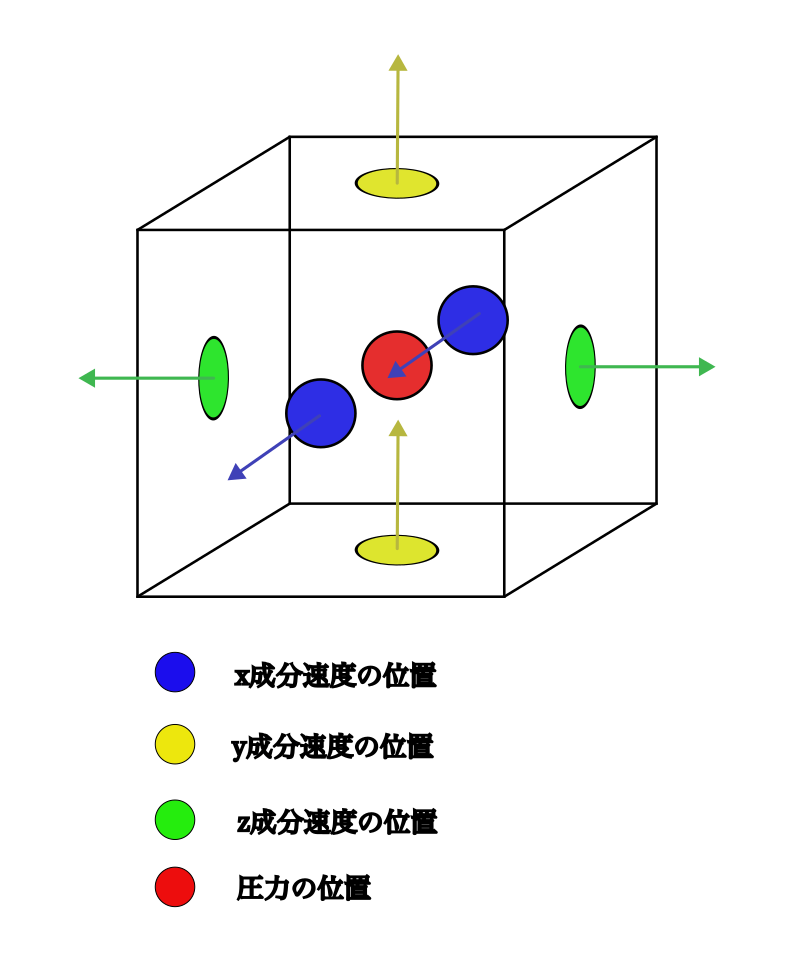
\includegraphics[width=80mm]{images/3dstaggerd.png}
\caption{スタッガード格子}
\label{fig:staggerd}
\end{center}
\end{figure}
格子法による空間の離散化は,扱う格子によって様々な手法が存在する.例えば物理量を格子の中心に配置するコロケート格子や,速度成分を格子の面の中心に配置するスタッガード格子が存在する.コロケート格子は流体の格子の形状によらず適用できるが,境界条件の設定が煩雑である.スタッガード格子は適用が立方体格子などに限定される一方,境界条件の設定が容易である.スタッガード格子は上の図\ref{fig:staggerd}のように,圧力の定義位置を格子の中心とし,格子面の中心にその格子面と垂直な流速の成分の位置を定義する.例えば$xy$平面に並行な格子面には,その地点での流速の$z$成分を配置する.

\section{部分空間法}\label{sec:Subspace}
部分空間法は,ベクトル空間をより低次元の部分空間に射影し,数値シミュレーションにおける計算負荷を軽減する手法である.流体シミュレーションにおける部分空間法は,モデル縮約やモデル縮退とも呼ばれている.扱うベクトルデータやシミュレーションの計算を低次元の部分空間に射影して行い計算負荷を軽減する.部分空間上におけるシミュレーションでは,元のシミュレーションよりも$\varDelta t$を小さい値に設定することで,シミュレーションの時間変化をより詳細に追跡することが可能である.以下では,部分空間法の理論の概要を説明する.

\subsection{部分空間への射影}
シミュレーションの前処理として,$n$次元ベクトル$\bm{x}$を$r$次元ベクトル$\bm{\widetilde{x}} $に変換する,$n \times r$直交行列$\bm{A}$を考える.直交行列の性質から,以下の2式が成り立つ.
 	\[
 		\bm{\widetilde{x}}  = \bm{A^{\mathsf T}}\bm{x}
 	\]
	\[
		\bm{x} = \bm{A}\bm{\widetilde{x}} 
	\]	
	また,$\bm{\widetilde{x'}}  = \bm{A^{\mathsf T}}\bm{x'}$を満たす$n$次元ベクトル$\bm{x'}$,$r$次元ベクトル$\bm{\widetilde{x'}} $について,以下の2式が成り立つような,任意の$m \times n$行列$\bm{F}$,任意の$m \times r$行列$\bm{\widetilde{F}}$を考える.
	\[
		\bm{x'} = \bm{F}\bm{x}
	\]
	\[
		\bm{\widetilde{x'}}  = \bm{\widetilde{F}}\bm{\widetilde{x}} 
	\]
$\bm{\widetilde{x'}}  = \bm{A^{\mathsf T}}\bm{x'}$に,$\bm{x'} = \bm{F}\bm{x}$と,$\bm{x} = \bm{A}\bm{\widetilde{x}} $を代入することで,
	\[
		\bm{\widetilde{x'}}  = (\bm{A^{\mathsf T}}\bm{F}\bm{A})\bm{\widetilde{x}} 
	\]
	が得られる.$\bm{\widetilde{x'}}  = \bm{\widetilde{F}}\bm{\widetilde{x}} $と比較すると,
	\[
	\bm{\widetilde{F}} = \bm{A^{\mathsf T}}\bm{F}\bm{A}
	\]
	が得られる.
	
以上により,任意のベクトルに対する行列積を,$n \times r$直交行列$\bm{A}$を用いて部分空間に射影することができる.

\subsection{スナップショット固有直交分解}
流体シミュレーションにおいて,部分空間に射影したベクトルを用いてシミュレーション計算をするためには,射影後のベクトルも流体の非圧縮性条件等の性質を満たさなければならない.そのような射影を達成する行列$\bm{A}$を得る手法として,スナップショット固有直交分解がある.行列$\bm{A}$を既存の流体のデータを主成分分析を用いて計算することで,流体の性質を満たした射影が可能である.
以降はスナップショット固有直交分解の具体的な計算方法について説明する.
	
	時刻$t \{t \in N, 0 \le t \le m\}$の$n$次元ベクトルデータ$\bm{u_t}$を用いて,$n\times m$行列$\bm{S}$を定義する.
		 \[ \bm{S} = 
        		\begin{bmatrix}
   | & | &  & |\\
   \bm{u}_0 & \bm{u}_1 &\cdots  & \bm{u}_{m-1} \\
   | & | &  & |
\end{bmatrix}
\]
次に,行列$\bm{S}$主成分分析を行うため,$n \times r$行列$\bm{A}$について以下の最小化問題を考える.ここで$r$は抽出したい主成分の数である.
\[
\text{min} || \bm{S} -  \bm{A}\bm{A^{\mathsf T}} \bm{S}||^2_F
\]


この最小化問題の解となる行列$\bm{A}$は,$\bm{S}\bm{S^{\mathsf T}}$の固有ベクトル$\bm{v_i}(0 \le i \le r-1)$を用いて,以下の行列になる.
 \[ 
 \bm{A}  = 
        		\begin{bmatrix}
   | & | &  & |\\
   \bm{v}_0 & \bm{v}_1 &\cdots  & \bm{v}_{r-1} \\
   | & | &  & |
\end{bmatrix}
\]
ここで,固有ベクトル$\bm{v_i}$に対応する固有値を$\lambda_i$は,$\lambda_0 \ge \lambda_1 \cdots \ge \lambda_i \ge \lambda_{n-1} $を満たすとする.$\bm{S}\bm{S^{\mathsf T}}$は対称行列になっているため,固有ベクトルは互いに直交し,$\bm{A^{-1}} = \bm{A^{\mathsf T}}$となる.%また,$n \times n$行列$\bm{S^{\mathsf T}}\bm{S}$ と$m\times m$行列$\bm{S}\bm{S^{\mathsf T}}$の固有ベクトルは

次に,行列$\bm{A}$を用いて$\bm{u}$を$\bm{\widetilde{u}}$に射影するとき,$\bm{\widetilde{u}}$が流体の非圧縮性条件$\nabla\boldsymbol{\cdot}\bm{\widetilde{u}} = 0$を満たしていることを確かめる.行列$\bm{S}$の各列ベクトル$\bm{u_i}$は既存のシミュレーションの速度データであるため,流体の非圧縮性条件$\nabla\boldsymbol{\cdot}\bm{u_i} = 0$を満たす.このことから,
\[
	\nabla\boldsymbol{\cdot}\bm{S}\ = \sum_{0 \le i \le n-1}\nabla\boldsymbol{\cdot}\bm{u_i} = 0
\]
が成り立つ.

また,行列$\bm{S}\bm{S^{\mathsf T}}$の固有ベクトル$\bm{v_i}$と,それに対応する固有値を$\lambda_i$とすると,固有値と固有ベクトルの定義から以下が成り立つ.
\[
	\bm{S}\bm{S^{\mathsf T}}\bm{v_i} = \lambda_i\bm{v_i}
\]
両辺に左から$\nabla\boldsymbol{\cdot}$を取ることにより,
\[
	(\nabla\boldsymbol{\cdot}\bm{S})\bm{S^{\mathsf T}}\bm{v_i} = \lambda_i\nabla\boldsymbol{\cdot}\bm{v_i}
\]
$\nabla\boldsymbol{\cdot}\bm{S}\ = 0$より,0でない$ \lambda_i$について,$\nabla\boldsymbol{\cdot}\bm{v_i} = 0$が成り立つことがわかる.$\bm{\widetilde{u}} = \bm{A^{\mathsf T}}\bm{u}$の第$i$成分は$\bm{v_i}\boldsymbol{\cdot}\bm{u}$であり,$\nabla\boldsymbol{\cdot}\bm{\widetilde{u}} =  0$が成り立つことがわかる.

$n \times n$行列$\bm{S}\bm{S^{\mathsf T}}$の主成分分析を行う代わりに,$\bm{S^{\mathsf T}}\bm{S}$の主成分分析を行い,$\bm{S}\bm{S^{\mathsf T}}$の固有値固有ベクトルを求めることができる.$\bm{S}\bm{S^{\mathsf T}}\bm{v_i} = \lambda_i\bm{v_i}$の両辺に左から$\bm{S^{\mathsf T}}$をかけることにより,
\[
	(\bm{S^{\mathsf T}}\bm{S})\bm{S^{\mathsf T}}\bm{v_i} = \lambda_i\bm{S^{\mathsf T}}\bm{v_i}
\]
を得る.行列$\bm{S^{\mathsf T}}\bm{S}$の固有値は,$\bm{S}\bm{S^{\mathsf T}}$の固有値と一致し,固有値$\lambda_i$対応する固有ベクトル$\bm{u_i}$について,$\bm{u_i} = \bm{S^{\mathsf T}}\bm{v_i}$であることがわかる.よって,$\bm{S^{\mathsf T}}\bm{S}$の主成分分析により得られた固有ベクトルと$\bm{S^{\mathsf T}}$の逆行列を用いて,$\bm{S}\bm{S^{\mathsf T}}$の主成分分析を行うことができる.

\subsection{特異値分解を用いる方法}
$n \times r$行列$\bm{S}$の特異値分解は,以下のように定義される.
\[
\bm{S} = \bm{U} \bm{\Sigma} \bm{V}^{\mathsf T}
\]
ここで,\( \bm{U} \) は \( n \times n \) のユニタリ行列であり,左特異ベクトルを列ベクトルとして持つ.\( \bm{V} \) は \( r \times r \) のユニタリ行列であり,右特異ベクトルを列ベクトルとして持つ.\(\bm{ \Sigma }\) は \( n \times r \) の対角行列であり,対角成分には特異値 \( \sigma_1, \sigma_2, \dots, \sigma_r \) が非負の降順で並ぶ.

以下に示す,行列$\bm{S^{\mathsf T}}\bm{S}$の固有値や固有ベクトルと行列$\bm{S}$の特異値分解の関係により,$\bm{S}\bm{S^{\mathsf T}}$の主成分分析を行う代わりに,行列\(\bm{S}\)の特異値分解を用いることができる.
行列$\bm{S^{\mathsf T}}\bm{S}$の対角化を,以下のように表す.
\begin{equation}\label{eq:diagonalization}
	\bm{S^{\mathsf T}}\bm{S} = \bm{P}\bm{A}\bm{P^{-1}}
\end{equation}
ここで,\(\bm{A}\)は\( n \times n \) の対角行列であり,対角成分には行列$\bm{S^{\mathsf T}}\bm{S}$の固有値が降順に並ぶ.\(\bm{P}\)の\(i\)列は固有値\(\bm{A_{i,i}}\)に対応する固有ベクトルである.
行列\(\bm{S}\)の特異値分解より,以下が成り立つ.
\[
\bm{S^{\mathsf T}}\bm{S} = (\bm{V} \bm{\Sigma} \bm{U}^{\mathsf T})(\bm{U} \bm{\Sigma} \bm{V}^{\mathsf T})
\]
行列\(\bm{U}\)はユニタリ行列,\(\bm{\Sigma}\)は対角行列であるから,
\[
\bm{S^{\mathsf T}}\bm{S} = \bm{V}\bm{\Sigma^2} \bm{V}^{\mathsf T}
\]
式\ref{eq:diagonalization}と右辺を比較することによって,\(\bm{P} = \bm{V} \),\(\bm{A} = \bm{\Sigma^2} \)であることがわかる.
\subsection{非線形項の計算}\label{noLinear}
非線形項については,立体求積法(Cubature Method)を用いた積分計算の計算量削減手法を用いて次元削減を行う.非線形関数$\mathcal{F}$について,$\bm{f} = \mathcal{F}(\bm{x})$とする.ここで,$\bm{f}$,$(\bm{x})$は$n$次元ベクトルである.削減前の$\bm{f}$は,$\mathcal{F}$をシミュレーション空間$\Omega$の全ての計算点$\bm{x_p}$において積分することで求められる.
\[
	\bm{f} = \int_\Omega\mathcal{F}_p(\bm{x_p})
\]
この積分計算を立体求積法を用いて次元削減する.
立体求積法はシミュレーション空間全域から適切に計算点を有限個サンプリングし,重み付き和をとることで積分計算を離散化する.
サンプリングした点集合を$P$,サンプリング点$p$に対応する重みを$w_p$とすると,立体求積法は以下のように表せる.
\[
	\bm{f} = \sum_{p=1}^Pw_p\mathcal{F}_p(\bm{x_p})
\]
この式は速度に関する基底を用いて以下のように部分空間へ射影することが可能である.
\[
	\bm{U_1}\bm{f} = \sum_{p=1}^Pw_p(\bm{U^p})^{\mathsf T}\mathcal{F}_p(\bm{U^p}\bm{x})
\]
ここで,$\bm{U^p}$は$3 \times n$基底行列$\bm{U}$のサンプリング点$p$に関する行を抜粋して作成した,$3 \times r$行列である.ここで,$\bm{\widetilde{f}}_p$ = $(\bm{U^p})^{\mathsf T}\mathcal{F}_p(\bm{\widetilde{u}})$とする.

以降はサンプリング点と重みを評価する手法について説明する.
サンプリングした点集合を$\bm{P}$とし,点集合の要素数を$P$とする.また,スナップショット数を$T$とする.以下の式を解の値が全て非負になるような線形ソルバであるNNLS(Non Negative Linear Solve)ソルバを用いることで,非負の$\bm{w}$が得られる.
\begin{equation}\label{weight}
	 \begin{bmatrix}
	 \bm{\widetilde{f}}^0_0	&\cdots	&\bm{\widetilde{f}}^p_0	&\cdots	&\bm{\widetilde{f}}^P_0\\
		\vdots		&\ddots		&\vdots		&		&\vdots			\\
	\bm{\widetilde{f}}^0_t	&\cdots	&\bm{\widetilde{f}}^p_t	&\cdots	&\bm{\widetilde{f}}^P_t\\
		\vdots		&		&\vdots			&\ddots		&\vdots			\\
	\bm{\widetilde{f}}^0_T	&\cdots	&\bm{\widetilde{f}}^p_T	&\cdots	&\bm{\widetilde{f}}^P_T\\
	\end{bmatrix}
	\begin{bmatrix}
	w_0 	\\
	\vdots \\
	w_p \\
	\vdots \\
	w_P
	\end{bmatrix}=
	\begin{bmatrix}
	\bm{\widetilde{f}}_0 	\\
	\vdots \\
	\bm{\widetilde{f}}_t \\
	\vdots \\
	\bm{\widetilde{f}}_T
	\end{bmatrix}
\end{equation}
ここで,$\bm{\widetilde{f}}_t $をシミュレーションのスナップショット行列$\bm{S}$から抜粋した$t$番目の速度$\bm{u}_t$を用いて$\bm{\widetilde{f}}_t = \bm{U}\bm{u}_t$とする.$\bm{\widetilde{f}}^p_t$はサンプリング点に関する値$\bm{U^p}\bm{u^p}_t$である.それぞれ次元削減後の速度ベクトルを表す.式\ref{weight}を線形方程式$\bm{A}\bm{w} = \bm{b}$とすると,$\bm{A}$は$rT\times P$行列である.
空集合の状態からランダムに点集合を選び,残差のノルム$||\bm{r}||_2 = ||\bm{b} - \bm{A}\bm{w}||_2$が閾値以下になるまでサンプリング点を追加する.サンプリングされた点を点集合に追加する際に,以下の式によって求められる確率関数を用いて追加するモンテカルロ法により,更なる効率化を達成できる.

\[
f(\bm{x_p}) = R(\frac{\bm{a_p}・\bm{r}}{\bm{r}・\bm{r}})
\]

上記の行列は
アルゴリズムの概略を以下に示す.

\begin{algorithm}[H]
    	\caption{Cubature random point sampling}
	\label{alg1}
        	\begin{algorithmic}[1]
		\STATE $P = \phi$,$\bm{r} = \bm{b}$と初期化する.                
		
		\WHILE{$||\bm{r}||_2 \le \epsilon$}
			\STATE ランダムに1つ$x_p$をサンプリングし,確率$p(\bm{x_p})$で$x_p$を$P$に追加する.
			\STATE \ref{weight}に従って,$\bm{A}\bm{w} = \bm{b}$を解く.
			\STATE 残差を次のように更新する.$\bm{r} = \bm{b} - \bm{A}\bm{w}$
			\STATE 重みが0となった点をPから削除する.
		\ENDWHILE
        \end{algorithmic}
\end{algorithm}

サンプリング点の集合と重みの計算にかかる計算量は,式\ref{weight}を$P$回解くため,$O(P\times rTP^2) = O(rTP^3)$である.
%$\bm{A}$を用いて$\bm{u}$を$\bm{\widetilde{u}}$に射影するとすると,$\bm{\widetilde{u}} = \bm{A^{\mathsf T}}\bm{u}$より,以下が成り立つ.
%\[
%	\bm{\widetilde{u}} =  \begin{bmatrix}
%	\bm{v_0}\boldsymbol{\cdot}\bm{u}\\
%	\bm{v_1}\boldsymbol{\cdot}\bm{u}\\
%	\vdots\\
%	\bm{v_r}\boldsymbol{\cdot}\bm{u}
%\end{bmatrix}
%\]
	%\subsection{}
	%\section{ボリュームデータの可視化手法}
\chapter{煙の流体シミュレーション}
流体シミュレーションを実施する際には,境界条件や外力項を適切に設定することで流体の挙動を制御することが可能である.特に,煙のような流体のシミュレーションにおいて,適切な外力を与えることで現実的な動きを再現できる.Fedkiwらによる手法\cite{fedkiw}は,高速かつ安定したシミュレーションを実現し,映像分野への応用が実用的になった最初の手法である.本章では,文献\cite{fedkiw}を参考に,フラクショナルステップ法を格子法により離散化した煙の流体シミュレーションの実装方法について述べる.さらに,スライスベースのボリュームレンダリングを用いた可視化手法についても説明する.%この手法で得られたシミュレーションデータを用いて部分空間法に用いるスナップショット固有直交分解を行う.

\section{格子法によるフラクショナルステップ法}
シミュレーション空間の$\rm{x,y,z}$軸方向の分割数を$\rm{nx,ny,nz}$とする.このとき空間解像度は$\rm{nx \cdot ny \cdot nz}$となり,速度の$\rm{x,y,z}$成分の空間解像度はそれぞれ$(nx+1) \cdot ny \cdot nz$,$nx \cdot (ny+1) \cdot nz$,$nx \cdot ny \cdot (nz+1)$となる.本論文では,$nx = ny =nz$とし,速度$\bm{v}$と圧力$\bm{p}$は以下のベクトルに離散化する.
\begin{itemize}
	\item	$\bm{v_x}$:$(nx+1) \times ny \times nz$次元ベクトル.
	\item	$\bm{v_y}$:$nx \times (ny+1) \times nz$次元ベクトル.
	\item	$\bm{v_z}$:$nx \times ny \times (nz+1)$次元ベクトル.
	\item	$\bm{v}$:$3\times(nx+1) \cdot ny \cdot nz $次元ベクトル.
	\item $\bm{p}$:$nx \cdot ny \cdot nz$次元ベクトル.
\end{itemize}
ここで$\bm{v}$の$0番目$から$(nx+1) \cdot ny \cdot nz -1$番目までの成分には速度の$x$成分,
$(nx+1) \cdot ny \cdot nz $から$2\times(nx+1) \cdot ny \cdot nz - 1$番目の成分には速度の$y$成分,
$2\times(nx+1) \dot ny \cdot nz - 1$から$3\times(nx+1) \cdot ny \cdot nz - 1番目の成分$には速度の$z$成分を保存する.
また,位置$\bm{x} =(i,j,k)$における速度$\bm{v} (\bm{x})$を,以下のように表す.
\[
	\bm{v} (\bm{x})= 
	 \begin{bmatrix}
		\bm{v_x}(i,j,k)\\
		\bm{v_y}(i,j,k)\\
		\bm{v_z}(i,j,k)
	\end{bmatrix}
\]
%前進差分を用いた空間の偏微分の離散化の例として,スタッガード格子を用いた以下の偏微分の離散化を上記のベクトルを用いて表現することを考える.
%\[\frac{\partial}{\partial \bm{x}}\bm{u} (\bm{x}) = \frac{\bm{u}(\bm{x}+\varDelta \bm{x})  - \bm{u} (\bm{x}) }{\varDelta \bm{x}}\]
%ここで,$\bm{u} (\bm{x})$は位置$\bm{x}$での速度を表す三次元ベクトルである.スタッガード格子の一辺の長さを$\varDelta L = \varDelta \bm{x}$,流体の位置ベクトル$\bm{x}$を自然数$i(0 \le i \le nx-1),j(0 \le j \le ny-1),k(0 \le k \le nz-1)を用いて,$$\bm{x} = (i\varDelta L,j\varDelta L,k\varDelta L)$とすると,以下のようになる.
%\[\frac{\bm{u}(\bm{x}+\varDelta \bm{x})  - \bm{u} (\bm{x}) }{\varDelta \bm{x}}= \begin{bmatrix}
%\frac{\bm{v_x}(i+1,j,k)  - \bm{v_x} (i,j,k) }{\varDelta L}\\
%\frac{\bm{v_y}(i,j+1,k)  - \bm{v_y} (i,j,k) }{\varDelta L}\\
%\frac{\bm{v_z}(i,j,k+1)  - \bm{v_z} (i,j,k) }{\varDelta L}
%\end{bmatrix}\]

\subsection{ディリクレ境界条件}
流体シミュレーションにおいて,流体と流体以外の境界面における物理量の条件を適切に設定する必要があり,これを境界条件と呼ぶ.文献\cite{fedkiw}では,境界における物理量を事前に一定の値に設定するディリクレ境界条件を採用しており,境界における物理量は$0$と設定される.ディリクレ境界条件は速度成分を逐次初期化することで適用可能であり,また,境界に対応する成分を$0$とした単位行列を用いて表現することもできる.この行列表現は通常の流体シミュレーションでは不要であるが,部分空間法を用いた流体計算において,境界条件を部分空間に射影するため,境界条件を行列積によって表現する手法が用いられている.ディリクレ境界条件を表現する行列を$\bm{D}$とすると,$\bm{D}$の$i,j$成分は以下のように定義される.
\begin{equation}
	\bm{D}_{i,j} = \begin{cases}
 	1 	& i = j かつ iは境界成分でない\\
 	0  		& その他\\
 \end{cases}
\end{equation}


\subsection{外力項計算}
外力項においては.再現したい現象に適した外力を与える必要がある.ユーザーが設定可能なパラメータによって外力を調整できる計算手法が望ましい.コンピュータグラフィックスにおける気体の外力には重力のほか,温度差による対流を発生させる力や.気体の渦運動を生成する力などが含まれ,これらを適用することで,気体の自然な挙動を再現することが可能となる.さらに,より現実的な挙動を再現するために,他の計算では定数として扱われる密度や温度を,本手法では位置および時刻に依存するスカラー量として計算する.

まず,気体に働く重力と,対流を発生させる力について説明する.位置$\bm{x}$における気体の密度,温度をそれぞれ$\rho(\bm{x})$,$T(\bm{x})$,環境温度を$T_{amb}(\bm{x})$,重力の方向ベクトルを$\bm{d}$とすると,気体に働く重力と,対流を発生させる力の合力$\bm{f}_{\text{buoy}}$は以下のように定義される.

\begin{equation}\label{eq:buoyancy}
	\bm{f_{\text{buoy}}(\bm{x})} =  \alpha \rho(\bm{x})\bm{d}+ \beta(T(\bm{x})- T_{amb}(\bm{x}))\bm{d}
\end{equation} 

ここで,$\alpha$,$\beta$はユーザーが設定するパラメータであり,それぞれ重力と対流の力の大きさを調整する.

次に,気体の渦運動を生成する力を説明する.
気体の渦運動を強めるために,渦度$\boldsymbol{\omega}$を利用した外力を考える.渦度は速度場$\bm{u}$の回転として以下のように定義される
\[
    \boldsymbol{\omega} = \nabla \times \bm{u}
\]
渦度の大きい領域では流体が強く回転しており,この回転運動を強調するために以下のような外力項$\bm{f}_{\text{vortex}}$を定義する
\[
    \bm{f}_{\text{vortex}} = \lambda (\boldsymbol{\omega} \times \bm{u})
\]
ここで,$\lambda$は渦運動を強調する強度を制御するパラメータである.この外力項は,渦度ベクトルと速度ベクトルの外積を利用することで,流れの回転を増幅する効果を持つ.

スタッガード格子における外力の配置位置は格子の中心であるため,流速の位置によって外力を補間して計算する.最終的な外力項計算は以下のようになる.
\begin{equation}
	\bm{u_0} =  \bm{u}  - \varDelta t(\bm{f}_{\text{buoy}} +  \bm{f}_{\text{vortex}} ) 
\end{equation} 

%!!!スタッガードグリッドのスキームが速度と外力で異なる話
%\begin{equation}\label{eq:confinent}
%	\bm{f_{conf}(\bm{x})} =  
%\end{equation} 

\subsection{移流項計算}
移流項は流体の物理量が流体の速度場によって移動する様を計算することができる.移流項は非線形方程式であり,様々な計算方法が存在する.本節ではコンピュータグラフィックスの分野において広く用いられている,文献\cite{stam}のSemi-Lagrangian法を紹介する.Semi-Lagrangian法は計算負荷が小さく,陰解法により安定した計算結果を得ることができる.

%Semi-Lagrangian法は移流計算を物質微分$\frac{\rm{D}}{\rm{D}t} =\frac{\partial}{\partial t} + \bm{u} (\bm{x},t)  \boldsymbol{\cdot}\nabla$を用いて行う.
%簡単のため,ナビエストークス方程式から粘性項と外力項を取り除いた,オイラー方程式と呼ばれるものについて考える.
Semi-Lagrangian法は,格子に配置されている計算点上の物理量を計算する格子法(Eulerian)の特徴と,移動する計算点を追跡し計算を行う粒子法(Lagrangian)の特徴を両方持っている計算手法である.
移流項の計算$$\bm{u_1} = \bm{u_0}  - \varDelta t (\bm{u_0}  \boldsymbol{\cdot}\nabla) \bm{u_0}$$を変形し,時刻の偏微分に対し前進差分$\frac{\partial \bm{u}}{\partial t} = \frac{\bm{u_1} - \bm{u_0}}{ \varDelta t }$すると,以下の式が得られる.
\[
\frac{\partial \bm{u}}{\partial t}   +(\bm{u_0}  \boldsymbol{\cdot}\nabla) \bm{u_0} = 0
\]
この式は以下の輸送方程式と呼ばれる式の特殊な場合であり,輸送方程式は一般の物理量$\phi$に関して適用可能である.
\begin{equation}\label{eq:transfer}
	\frac{\partial {\phi}}{\partial t}  +(\bm{u}  \boldsymbol{\cdot}\nabla) {\phi} = 0
\end{equation} 
この輸送方程式が成り立つとき,位置$\bm{x}$,時刻$t$における物理量$\phi(\bm{x},t)$について,以下の式が成り立つ.
\begin{equation}\label{eq:semi-Lagrangian}
	{\phi}(\bm{x},t) = {\phi}(\bm{x}  - \varDelta t \bm{u},t)
\end{equation} 
Semi-Lagrangian法を以下のように流速に適用することで移流項の計算を行う.また,密度や温度などに対して適用することで,空間の速度ベクトル場に沿って気体が運動する様子を再現することができる.
\[
	\bm{u_1}(\bm{x}) = \bm{u_0}(\bm{x}  - \varDelta t \bm{u_0})
\]
以下では,輸送方程式\ref{eq:transfer}が成り立つとき,式\ref{eq:semi-Lagrangian}が成り立つことを確認する.$\bm{x}$にある物理量は$\bm{u} (\bm{x}) $に沿って$\varDelta t\bm{u} (\bm{x})$移動すると仮定すると,移動前の物理量は$\phi(\bm{x} -  \varDelta t\bm{u} (\bm{x}))$となる.この間の物理量の変化$\varDelta {\phi}$は以下のようになる.
\[
\varDelta \phi = \phi( \bm{u} (\bm{x}),t) - \phi (\bm{x} - \varDelta t\bm{u} (\bm{x}),t)
\]
これを一次のテイラー展開を用いて表すと,
\[
\varDelta \phi   = \frac{\partial \bm{u} (\bm{x}) }{\partial \bm{x}}\phi (\bm{x},t) \varDelta t + \frac{\partial \phi (\bm{x},t) }{\partial t}\varDelta t
\]
$\frac{\partial \bm{u} (\bm{x}) }{\partial \bm{x}}\phi (\bm{x},t)= (\bm{u}(\bm{x}) \boldsymbol{\cdot}\nabla)\phi(\bm{x},t)$より,
\[
 \frac{\varDelta \phi}{\varDelta t} =  (\bm{u}(\bm{x})\boldsymbol{\cdot}\nabla) \phi(\bm{x},t) + \frac{\partial \phi(\bm{x},t) }{\partial t}
 \]
 
 右辺が輸送方程式\ref{eq:transfer}になっていることから,$ \varDelta \phi =0$が成り立つ.
$\varDelta \phi = \phi( \bm{u} (\bm{x})) - \phi (\bm{x} - \varDelta t\bm{u} (\bm{x}))= 0$より,式\ref{eq:semi-Lagrangian}が成り立つことが確認できる.
\subsection{粘性項計算}
粘性項は以下の式を用いて,流体が徐々に周囲に広がっていく様を計算することができる.
\[
\bm{u_2}   =  \bm{u_1} - \varDelta t \nu\nabla^2\bm{u_1}
\]
$\nabla^2$を離散ラプラシアン行列$\bm{L}$を用いて離散化することができるため,粘性項計算は以下のように表すことができる.
\begin{equation}\label{eq:discrete Laplacian}
	\bm{u_2}   =  \bm{u_1} - \varDelta t \nu\nabla^2\bm{u_1} = (\bm{I} -  \frac{\varDelta t \nu}{(\varDelta x)^2}\bm{L})\bm{u_1}
\end{equation}
ここで,$v_0$から$v_{n-1}$の$n$個の頂点を持つ無向グラフに対して$n \times n$行列$\bm{L}$の成分$\bm{L}_{i,j}$は以下のように定義される.ただし,無向グラフは自己ループを持たないとする.
\[
	\bm{L}_{i,j} = \begin{cases}
 	deg(v_i) 	& i = j\\
 	-1  		& v_iとv_jが接続している\\
 	0  		& その他\\
 \end{cases}
\]
スタッガード格子を用いた流体シミュレーションにおいて,無向グラフは流体のそれぞれの速度成分ごとの連結成分を持つとする.本論文のシミュレーションにおいては連結成分数は3であり,それぞれの頂点数は$(nx+1) \times ny \times nz$である.また,シミュレーション境界を除いて,速度に対応する次数は$6$である.シミュレーション境界に対応する離散ラプラシアン行列の成分については,ディリクレ境界条件によって速度成分が$0$になるため,任意の値でよい.

粘性項計算を$\bm{u_2}   =  \bm{V}\bm{u_1}$と表現する行列を$\bm{V}$とすると,の成分$\bm{V}_{i,j}$は以下のように定義される.
 \[
 	\bm{V}_{i,j}  = \begin{cases}
 	1 - 6 \frac{\varDelta t \nu}{(\varDelta x)^2} 	& i = j\\
 	 \frac{\varDelta t \nu}{(\varDelta x)^2}  	& v_iとv_jが接続している\\
 	0  				& その他\\
	 \end{cases}
\]

\subsection{圧力項計算}
圧力項計算は,流体の非圧縮性を満たすように流体に圧力勾配による外力を与える計算である.本節では,代表的な圧力項計算手法であるコリンの射影法\cite{Chorin}を紹介する.
コリンの射影法は以下の式を満たす圧力$\bm{p}$を求める.
\[
	\bm{u} (t + \varDelta t)=  \bm{u_2} - \varDelta t \frac{1}{\rho}\nabla p
\]
上記の式の両辺の発散をとると,
\[
	\nabla\boldsymbol{\cdot}\bm{u} (t + \varDelta t)=  \nabla\boldsymbol{\cdot}\bm{u_2} - \varDelta t \frac{1}{\rho}\nabla^2 p
\]
が得られる.流体の非圧縮性条件,$\nabla\boldsymbol{\cdot}\bm{u} (t + \varDelta t)= 0$により,左辺は0になるため,
\begin{equation}
\nabla\boldsymbol{\cdot}\bm{u_2} = \frac{\varDelta t}{\rho}\nabla^2 p
\end{equation} 
が得られる.この式を圧力に関するポアソン方程式として解き,$\bm{u} (t + \varDelta t)=  \bm{u_2} - \varDelta t \frac{1}{\rho}\nabla p$に代入することで,圧力勾配による速度変化を計算する.ポアソンの境界条件にはディリクレ境界条件を適用する.

%スタッガード格子では圧力と流速の配置されている位置が異なるため,空間微分に対して同じ差分は適応できない.そこで両辺をセルの領域で積分することを考える.
%\[
%\int_V\nabla\boldsymbol{\cdot}\bm{u_2} dV= \int_V\frac{\varDelta t}{\rho}\nabla^2 \bm{p}  dV
%\]
%右辺にガウスの発散定理を適用すると,周回積分の形で表せる.
%\[
%\oint_V\bm{u_2}\boldsymbol{\cdot}\bm{n} dV= \oint_V\frac{\varDelta t}{\rho}\nabla \bm{p}  \boldsymbol{\cdot}\bm{n}dV
%\]
%左辺から空間微分が消去できたため,右辺の空間微分に対して適切な微分スキームを適用することで,周回積分を離散化することができる.ここで離散化のため,$x軸方向にi番目,y軸方向にj番目,z軸方向にk番目の格子を$$g_{i,j,k}$,圧力を$p_{i,j,k}$と定義し,図\ref{fig:pressure_model}のようなモデルを考える.

%まず,整数$n=0,1,2,\cdots 5$までを,それぞれ格子の各面の方向に割り振る.図\ref{fig:pressure_model}の場合,$n=0$は$x$軸正の方向,$n=1$は$y$軸正の方向,$n=2$は$x$軸負の方向,$n=3$は$y$軸負の方向,$n=4$は$z$軸正の方向,$n=5$は$z$軸負の方向に割り振る.ここで,この整数$n$を用いて,以下の配列や変数を定義する.
%\begin{quote}
%	\begin{itemize}
%		\item $F_n$ 格子の面の各方向に隣接しているものが流体なら$1$,壁面なら$0$を取るブーリアン値.
		
%		図\ref{fig:pressure_model}の場合,$n=0$に対応する$x$軸正の方向と,$n=5$に対応する$z$軸負の方向は壁に隣接していて格子がないため,$F_0,F_5 = 0,F_1,F_2,F_3,F_4 = 1$となる.
%		\item $D_n$ 格子の面の各方向に垂直で,格子の外側を向く単位ベクトルを表す係数.向いている方向が座標軸の正の向きなら+1,					負の向きなら$-1$を取る整数値.
		
%		図\ref{fig:pressure_model}の場合,座標軸の正の方向に向いているのは$n=0,n=1,n=4$に対応する方向で,それ以外は負の方向に向いているため,
%		$F_0,F_1,F_4 = 1,F_2,F_3,F_4 = -1$となる.
%		\item $p_n$ 割り振られた方向に隣り合っている格子の圧力値.
%		図\ref{fig:pressure_model}の場合,$p_0 = p_{i+1,j,k}$,$p_1 = p_{i,j+1,k}$,$p_2 = p_{i-1,j,k}$,$p_3 = p_{i,j-1,k}$,$p_4 = p_{i,j,k+1}$,$p_5 = p_{i,j,k-1}$となるが,境界条件を考えると,壁に隣接している格子との圧力値の勾配を$0$にするため,$p_0 = p_{i,j,k}$,$p_5 = p_{i,j,k}$である.
%		\item $\nabla p_n$ 割り振られた方向の圧力勾配.前方差分によって,$\nabla p_n (\bm{x},t)  = \frac{p_n - p_{i,j,k}}{\varDelta x}$と近似できる.
%		\item $u_n$ $g_{i,j,k}$において,割り振られた方向の格子面に配置されている流速値.壁に隣接している方向は流速を$0$にするため,$u_0 = 0$,$u_5 = 0$である.
%	\end{itemize}
%\end{quote}
%\begin{figure}[htbp]
%\begin{figure}[H]
%\begin{center}
%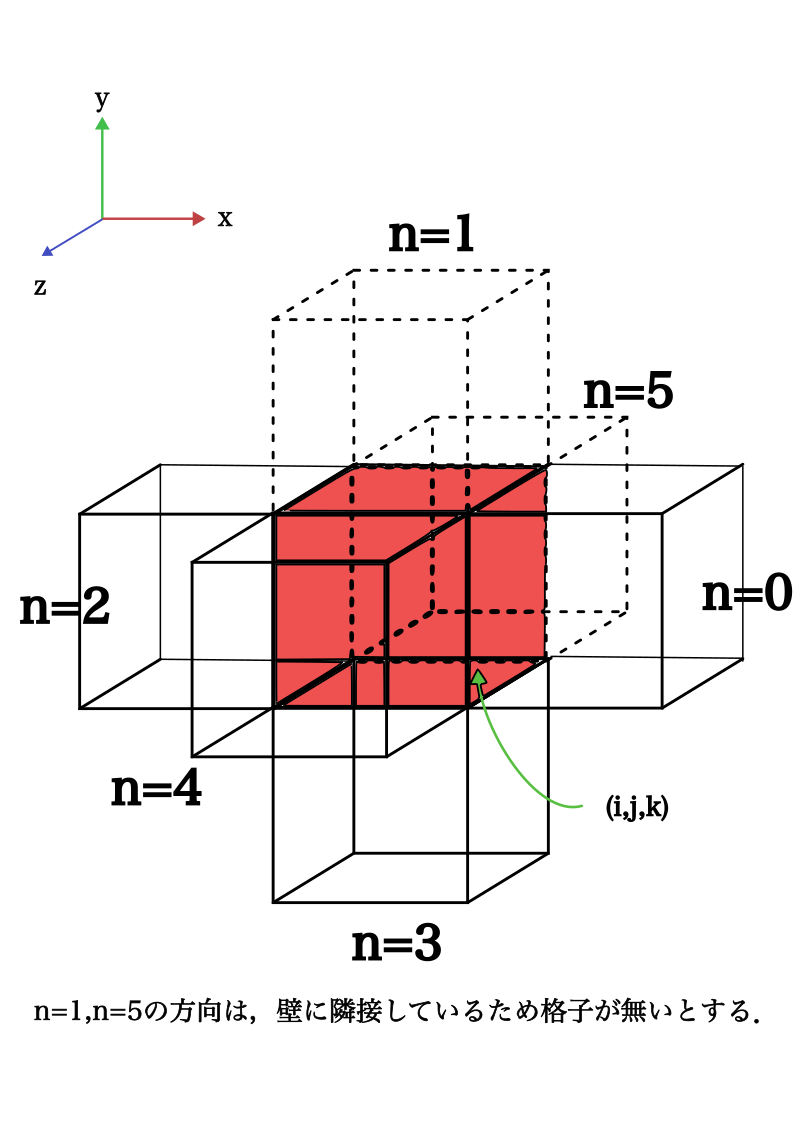
\includegraphics[width=80mm]{images/pressure_model.png}
%\caption{圧力計算のモデル}
%\label{fig:pressure_model}
%\end{center}
%\end{figure}
%定義した配列や変数を用いて,周回積分の形で表された式を離散化することで,下記の式を得る.
%\[
%	\sum_{n}\frac{\varDelta t}{\rho}\nabla p_n (\bm{x},t) F_n =  \sum_{n}u_nD_nF_n
%\]


%が得られ,圧力勾配を$\nabla p_n (\bm{x},t)  = \frac{p_n - p_{i,j,k}}{\varDelta x}$で近似すると,

%\[
%\sum_{n}\frac{\varDelta t}{\rho}\frac{p_n (\bm{x},t) - p_{i,j,k} (\bm{x},t) }{\varDelta \bm{x}}F_n\varDelta x =  \sum_{n}\bm{u_n}^*D_nF_n\varDelta x
 %\]
%が得られる.この式を整理すると,
%\begin{equation}\label{eq:discretized_pressure}
%\sum_{n}\frac{\varDelta t}{\rho}\frac{p_n (\bm{x},t)  - p_{i,j,k} (\bm{x},t) }{\varDelta \bm{x}}F_n = \sum_{n}\bm{u_n}^*D_nF_n
%\end{equation} 
%が得られる.
圧力項は圧力を変数とした,上記の式を$\bm{Ax=b}$に対応させたものを解く.空間解像度を$n$とすると,$\bm{A}$は$n \times n$行列であり,$\bm{b}$は$n$次元ベクトルである.以下では上記の式の離散化方法について説明する.行列$\bm{A}$は式\ref{eq:discrete Laplacian}と同様に離散ラプラシアンを用いて$\bm{A} = \frac{\varDelta t}{\rho \varDelta x}\bm{L}$と計算できる.よって,$\bm{A}$の$(i,j)$成分$\bm{A_{i,j}}$の各成分は以下のように定義される.

\[
	\bm{A}_{i,j} = 
	\begin{cases}
 	6\frac{\varDelta t}{\rho \varDelta x} 	& i = j\\
 	-\frac{\varDelta t}{\rho \varDelta x}   	& v_iとv_jが接続している\\
 	0  							& その他\\
	\end{cases}
\]
次に,ベクトル$\bm{b}$の計算方法について説明する.
3次元のスタッガード格子における流体シミュレーションでは,速度場 $\bm{u} = (u_x,u_y,u_z)
$ の発散 $\nabla \cdot \bm{u}$ を行列 $\bm{W}$ を用いて

\[
\nabla \cdot \bm{u} = \bm{W} \bm{u}
\]

と離散化する.3次元のスタッガード格子では,発散は以下の中央差分で近似される.

\[
\nabla \cdot \bm{u} \approx \frac{u_x(i+1,j,k) - u_(i,j,k)}{\varDelta x} + \frac{u_y(i,j+1,k)- u_y(i,j,k)}{\varDelta y} + \frac{u_z(i,j,k+1) - u_z(i,j,k)}{\varDelta z}
\]
ただし,本実験では$\varDelta x = \varDelta y= \varDelta z$である.
これを行列形式で表現するために,行列 $\bm{W}$ の各成分 $W_{i,j}$ を次のように定義する.

\begin{equation}
W_{i,j} =
\begin{cases}
\frac{1}{\varDelta x}, &  u_x(i+1,j,k),u_y(i,j+1,k),u_z(i,j,k+1)に対応する成分 \\
-\frac{1}{\varDelta x}, & u_x(i,j,k),u_y(i,j,k),u_z(i,j,k)に対応する成分\\
0, & \text{otherwise}
\end{cases}
\end{equation}

以上により,ベクトル$\bm{b}$は速度ベクトル$\bm{u_2}$と行列$\bm{W}$を用いて,$\bm{b} = \bm{W}\bm{u_2}$と表せる.したがって,実際に解く線形方程式は$\bm{A}\bm{p} = \bm{W}\bm{u_2}$となる.

行列$\bm{A}$は規模が大きいため,反復法を用いて計算する.$\bm{A}$のほとんどの成分は$0$であるため,疎行列の反復法ソルバーを用いることで空間計算量や時間計算量を削減できる.反復法では,必要な精度に解が収束したら計算を打ち切る.ここでの精度は反復回数や視覚的に影響を与えるほか,低い精度では流体の非圧縮性条件を満たさなくなってしまう恐れがある.行列$\bm{A}$が正定値対称行列になるため,前処理付き共役勾配法が広く用いられている.文献\cite{fedkiw}のフラクショナルステップ法における計算時間のボトルネックは圧力項計算であり,解の収束が早いほど反復回数が少なくなり,計算負荷が少なくなる.

次に,圧力の勾配ベクトル$\nabla\bm{p}$が速度に与える影響を考える.
圧力勾配を行列 $\bm{Y}$ を用いて離散化し,以下のように表せることを説明する.

\begin{equation}
\nabla p = \bm{Y} p
\end{equation}

3次元格子では,圧力勾配 $\nabla p = (\frac{\partial p}{\partial x}, \frac{\partial p}{\partial y}, \frac{\partial p}{\partial z})$ は,各方向において以下のように離散化される:

\begin{equation}
\frac{\partial p}{\partial x} \approx \frac{p_{i+1,j,k} - p_{i,j,k}}{\Delta x}, \quad
\frac{\partial p}{\partial y} \approx \frac{p_{i,j+1,k} - p_{i,j,k}}{\Delta y}, \quad
\frac{\partial p}{\partial z} \approx \frac{p_{i,j,k+1} - p_{i,j,k}}{\Delta z}
\end{equation}

ただし,本実験では$\varDelta x = \varDelta y= \varDelta z$である.
これを行列形式で表現するために,行列 $\bm{Y}$ の各成分 $Y_{m,n}$ を次のように定義する.

\[
Y_{m,n} =
\begin{cases}
\frac{1}{\varDelta x}, &  \nabla p_x(i+1,j,k),\nabla p_y(i,j+1,k),\nabla p_z(i,j,k+1)に対応する成分 \\
-\frac{1}{\varDelta x}, &  \nabla p_x(i,j,k), \nabla p_y(i,j,k), \nabla p_z(i,j,k)に対応する成分\\
0, & \text{otherwise}
\end{cases}
\]

この行列 $\bm{Y}$ を用いることで,速度場の更新に必要な圧力勾配を効率的に計算することが可能となる.%また,$\bm{Y}$は$\bm{W}$ の転置になっている.

%\begin{figure}[htbp]
%\begin{figure}[H]
%\begin{center}
%\includegraphics[width=80mm]{images/P2V.png}
%\caption{圧力と速度の配置位置}
%\label{fig:pressure_model}
%\end{center}
%\end{figure}

以上のことから,圧力項の計算をまとめると,以下のようになる.
\[
	\bm{b} = \bm{W}\bm{u_2}
\]
\[
	\bm{p} = \bm{A^{-1}}\bm{b}
\]
\[
	\bm{u_3}  =  \bm{u_2} - \bm{Y}\bm{p} 
\]

\section{ボリュームデータの可視化手法}
ボリュームデータを三次元的な広がりの様子を把握できるようにレンダリングする手法をボリュームレンダリングという.描画対象の表面のみをレンダリングするサーフェスレンダリングとは異なり,光の散乱や吸収などの光学的性質を利用して,描画対象の内側のデータも出力画像に反映させる.代表的な手法として,サンプルデータをスライスごとに投影するスライスベースの手法が存在する.スライスベースの手法は計算負荷が低くリアルタイム処理に適している.本章では,スライスベースのボリュームレンダリングのアルゴリズムと,各スライスのテクスチャの計算方法を紹介する.

スライスベースのボリュームレンダリングは,シミュレーション空間がボクセル空間として捉えられることを利用し,気体の密度を用いてボクセルの透明度や色を計算する.その後,シミュレーション空間をボクセルの透明度や色をテクスチャとしてマッピングした複数の平面(スライス)に分割し,それらを順次描画することで最終的な画像を生成する.以下では,ボクセルの透明度と,最終的な画像の画素値を計算する方法を説明する.

視線方向に沿ったスライス間の距離を$\varDelta s$とし,$i$番目のスライスと視線の交点の位置を$i\varDelta s$とする.
ボクセルの透明度$t(i\varDelta s)$と不透明度$\alpha( i\varDelta) $は,以下の式で計算する.
\[t( i\varDelta s) = \text{exp}( -\rho(i\varDelta s) \varDelta s)\]
\[\alpha( i\varDelta s) = 1 - t( i\varDelta s) \]
$\rho(i\varDelta s)$は,流体シミュレーションによって計算した,位置$i\varDelta s$の密度である.
また,$\varDelta s$は視線とスライスの法線がなす角$\theta$とすると以下のように変化するため,$\varDelta s$はテクスチャ座標によって異なる.
%
\begin{equation}\label{eq:cos}
%\varDelta s' = \frac{\varDelta s}{cos\theta}
\varDelta s' = \varDelta s / \text{cos}\theta
\end{equation}

透明度を考慮するレンダリング手法の代表的なものとして,アルファブレンディングが存在する.アルファブレンディングは以下の式で計算する.
\begin{equation}\label{eq:alpha}
I_n( \bm{x}) = \alpha_n( \bm{x}) c_n( \bm{x}) + ( 1-\alpha_n( \bm{x}) ) I_{n-1}( \bm{x}) 
\end{equation}
\begin{itemize}
	\item $I_n( \bm{x}) $: n番目のスライスの位置$\bm{x}$における累積輝度
	
	\item $c_n( \bm{x}) $: n番目のスライスの位置$\bm{x}$における輝度
	
	\item $\alpha_n( \bm{x}) $: n番目のスライスの位置$\bm{x}$における不透明度

\end{itemize}
%
式\ref{eq:alpha}の不透明度に$\alpha( i\varDelta s') $を用いることで,アルファブレンディングによってシミュレーション空間がボリュームレンダリングできる.

ここで,シミュレーション空間をスライスによって分割する方向は,視線方向に垂直な方向と,$\rm{x,y,z}$軸の中で視線になるべく垂直な方向が考えられる.一般的に視線とスライスの交点がボクセルの計算点上にないため,$\rho( i\varDelta s) $を補間して得る必要がある.前者は式\ref{eq:cos}による$\varDelta s$の変化量が透視投影の影響しか受けない.一方,後者は視線とスライスの法線がなす角は視点に依存し,より式\ref{eq:cos}による$\varDelta s$の変化量が大きい.また,$\rm{x,y,z}$軸の方向による分割は視線の方向によって視線と交差するスライスが少なくなり,視覚的に不自然なスライスの形状が現れることがある.CGの分野においては後者の手法でも見た目上問題ないことが多く,文献\cite{fedkiw}では後者の手法を用いている.

%\begin{algorithm}[H]
%    	\caption{Axis Alined slice-based Volume Rendering}
%	\label{alg1}
%        	\begin{algorithmic}[1]
%		\STATE x,y,z軸の中から,視線方向に近いものを選ぶ.
%                 \STATE 軸に垂直な平面(スライス)を,アルファブレンディングして描画.
%                 \[{\rm{I_n}}(\bm{x})= \alpha_n(\bm{x})c_n(\bm{x}) + (1-\alpha_n(\bm{x})){\rm{I_{n-1}}}(\bm{x})\]
%                 \[\alpha(\bm{x}) = 1 - exp(-\rho(\bm{x})\varDelta s)\]
%        \end{algorithmic}
%\end{algorithm}

\chapter{部分空間法とスナップショット分割による高速化} \label{chapter:3}
本章では,スタッガード格子を用いた煙の流体シミュレーション\cite{fedkiw}に対して,線形項と非線形項の計算を部分空間上に射影して計算する既存手法\cite{subspace}を適用する方法を説明する.その後,スナップショットを分割する手法を提案する.部分空間法の前処理において,基底の計算と行列の射影の計算量はスナップショット数の$2$乗に比例し,前処理の大多数の時間を占めている.スナップショットを分割することで前処理の計算の高速化が期待できる.
\section{基底空間構築手法}
スタッガード格子を用いた流体シミュレーションの,時刻$t \{t \in N, 0 \le t \le m\}$の流速データ$\bm{u_t}$と圧力データ$\bm{p}$を用いて,以下のスナップショット行列$\bm{S_u}$と$\bm{S_p}$を定義する.
 \[ \bm{S_u} = 
	 \begin{bmatrix}
  	 | & | &  & |\\
  	 \bm{u}_0 & \bm{u}_1 &\cdots  & \bm{u}_{m-1} \\
   	| & | &  & |
	\end{bmatrix}
\]
 \[ \bm{S_p} = 
	 \begin{bmatrix}
  	 | & | &  & |\\
  	 \bm{p}_0 & \bm{p}_1 &\cdots  & \bm{p}_{m-1} \\
   	| & | &  & |
	\end{bmatrix}
\]
ここで,$\rm{x,y,z}$軸方向の分割数を$\rm{nx,ny,nz}$$(nx = ny = nz)$とすると,$\bm{u_t}$と$\bm{p}$の次元はそれぞれ$3(nx+1)\times nx\times nx$,$nx\times nx \times nx$である.
スナップショット行列は空間計算量が大きく,直接特異値分解を適用すると空間計算量の制約を満たさない場合がある.これを避けるため,QR分解を利用する手法を説明する.また,特異値分解を用いた次元削減はの条件数は,行列を構成する列ベクトル同士の相関が強いほど悪くなることが知られている.スナップショット行列はデータ間に相関があるため,直接特異値分解を適応すると条件数が大きくなり,計算が不安定になる問題を緩和することができる.

まず,$n \times m$行列$\bm{S}$を以下のようにQR分解する.
\[
	\bm{S} = \bm{Q}\bm{R}
\]
ここで,行列$\bm{Q}$は$n \times m$直交行列であり,行列$\bm{R}$は$m \times m$上三角行列である.
その後,行列$\bm{R}$を以下のように特異値分解する.
\[
\bm{R} = \bm{U_R} \bm{\Sigma_R} \bm{V_R}^{\mathsf T}
\]

ここで,$\bm{S^{\mathsf T}}\bm{S}$を計算する.
\[
	\bm{S^{\mathsf T}}\bm{S} =  \bm{V_R}  \bm{\Sigma_R}^{\mathsf T} \bm{U_R}^{\mathsf T}\bm{Q}^{\mathsf T} (\bm{Q}\bm{U_R} \bm{\Sigma_R} \bm{V_R}^{\mathsf T})
\]
$\bm{Q}と\bm{U_R}$は直交行列であることから,以下が得られる.

\[
\bm{S^{\mathsf T}}\bm{S} = \bm{V_R}\bm{\Sigma_R^2} \bm{V_R}^{\mathsf T}
\]

\ref{sec:Subspace}にて
$\bm{S^{\mathsf T}}\bm{S} = \bm{V}\bm{\Sigma^2} \bm{V}^{\mathsf T}$
となることを利用して基底を求めることができることを紹介した.同様にしてQR分解後の特異値分解を利用して基底を求めることができる.この手法により,特異値分解する行列は各列に相関がある$n \times m$行列からQR分解後の$m \times m$上三角行列になり,空間計算量と行列の条件数が改善される.

\section{フラクショナルステップ法への部分空間法の適用}
本節では,\ref{sec:fractional}にて得たフラクショナルステップ法による以下のシミュレーション計算に,部分空間法を適用する方法を説明する.

%\begin{equation}
%	\bm{u_0} =  \bm{u} (t)  - \varDelta t \bm{f} 
%\end{equation} 

%\begin{equation}
%	\bm{u_1} (\bm{x}) = \bm{u_0} (\bm{x}) - \varDelta t (\bm{u_0}(\bm{x})  \boldsymbol{\cdot}\nabla) \bm{u_0}(\bm{x})
	%\bm{u_1}(\bm{x}) = \bm{u_0}(\bm{x}  - \varDelta t \bm{u_0})
%\end{equation}
\[
	\bm{u_0} =  \bm{u} (t)  - \varDelta t \bm{f} 	
\]
\[
	\bm{u_1}(\bm{x}) = \bm{u_0}(\bm{x}  - \varDelta t \bm{u_0})
\]
\[
	\bm{u_2}   =  \bm{V}\bm{u_1}
\]
\[
	\bm{b} = \bm{W}\bm{u_2}
\]
\[
	\bm{p} = \bm{A^{-1}}\bm{b}
\]
\[
	\bm{u_3}  =  \bm{u_2} - \bm{Y}\bm{p} 
\]
フラクショナルステップ法では,中間子$\bm{u_0}$から$\bm{u_3}$までの4種類の速度ベクトルを計算する.それぞれの速度ベクトルを部分空間に射影するため,対応したスナップショット行列が1つずつ必要である.中間子$\bm{u_i}$から得た基底を$\bm{U_i}$,$\bm{p}$から得られた基底を$\bm{P}$とする.
フラクショナルステップ法の線形項の計算を部分空間に射影すると,以下のようになる.
%\[
%\begin{aligned}
%	\bm{U_2^{\mathsf T}}\bm{u_2}   =  (\bm{U_2^{\mathsf T}}\bm{V}\bm{U_1})\bm{U_1^{\mathsf T}}\bm{u_1}				& \bm{\widetilde{u_2}} = \bm{\widetilde{V}}\bm{\widetilde{u_1}\\
%	\bm{P^{\mathsf T}}\bm{b} = (\bm{P^{\mathsf T}}\bm{W}\bm{U_2})\bm{U_2^{\mathsf T}}\bm{u_2}						&a\\
%	\bm{P^{\mathsf T}}\bm{p} = (\bm{P^{\mathsf T}}\bm{A^{-1}}\bm{P})\bm{P^{\mathsf T}}\bm{b}						&b\\
%	\bm{U_3^{\mathsf T}}\bm{u_3}  =  \bm{U_2^{\mathsf T}}\bm{u_2} - (\bm{U_3^{\mathsf T}}\bm{Y}\bm{P})\bm{P^{\mathsf T}}\bm{p}&c
%\end{aligned}
%\]
\begin{align*}
 \bm{U_2^{\mathsf T}}\bm{u_2}	& = (\bm{U_2^{\mathsf T}}\bm{V}\bm{U_1})\bm{U_1^{\mathsf T}}\bm{u_1} 					&\bm{\widetilde{u_2}} 		&= \bm{\widetilde{V}}\bm{\widetilde{u_1}}	\\
 \bm{P^{\mathsf T}}\bm{b}		& = (\bm{P^{\mathsf T}}\bm{W}\bm{U_2})\bm{U_2^{\mathsf T}}\bm{u_2}        				&\bm{\widetilde{b}}			&= \bm{\widetilde{W}}\bm{\widetilde{u_2}}	\\
 \bm{P^{\mathsf T}}\bm{p} 		&= (\bm{P^{\mathsf T}}\bm{A}^{-1}\bm{P})\bm{P^{\mathsf T}}\bm{b}						&\bm{\widetilde{p}}			&= \bm{\widetilde{A}}\bm{\widetilde{b}}\\
 \bm{U_3^{\mathsf T}}\bm{u_3} 	&=  \bm{U_2^{\mathsf T}}\bm{u_2} - (\bm{U_3^{\mathsf T}}\bm{Y}\bm{P})\bm{P^{\mathsf T}}\bm{p}	&\bm{\widetilde{u_3}}		&= \bm{\widetilde{u_2}}  -  \bm{\widetilde{Y}}\bm{\widetilde{p}}
\end{align*}
ただし,$\bm{P^{\mathsf T}}\bm{A}^{-1}\bm{P} = (\bm{P^{\mathsf T}}\bm{A}\bm{P})^{-1}$であり,圧力ベクトルの次元数を$n$として$\bm{A}$は$n\times n$疎行列であり,$(\bm{P^{\mathsf T}}\bm{A}\bm{P})$は$m\times m$密行列である.密行列であることに注意が必要だが,逆行列を高速に求められるため,$\bm{\widetilde{A}} = (\bm{P^{\mathsf T}}\bm{A}\bm{P})^{-1}$とする.

部分空間法によるシミュレーション計算は,前処理として基底と部分空間に射影した行列を計算する.基底を計算するステップの計算量のボトルネックは,QR分解の$O(nm^2)$である.部分空間に射影した行列を計算するステップについては,射影前のそれぞれの行列が非常に疎であるため,基底の計算ほど時間はかからない.

非線形項は\ref{noLinear}にて紹介した立体求積法を用いて計算する.立体求積法に用いる基底は,外力項は$\bm{U}_0$であり,移流項は$\bm{U}_1$である.
例えば,移流項を最終的な部分空間に射影した移流項計算は以下のようになる.
\[
	\bm{\widetilde{u_2}} = \sum_{p=1}^Pw_p\bm{\widetilde{f}}_p =   \sum_{p=1}^Pw_p(\bm{U^p_1})^{\mathsf T}\mathcal{F}_p(\bm{\widetilde{u_1}})
\]

\section{部分空間法の課題}
部分空間法はシミュレーションの次元を$n$次元から$r$次元に削減するため,各ステップの計算負荷を大幅に減らすことができる手法である.その一方で,前処理として基底の計算や立体求積法のランダムサンプリングと重み計算,シミュレーションに用いる行列の部分空間への射影などを行う必要がある.これらの計算負荷はスナップショットの数に依存しているが,スナップショットの数以下の次元にしか次元削減できず,流体シミュレーションとして意味のある結果を得るためにはスナップショットの数が十分でなければならない.また,スナップショット行列の空間解像度が大きいという問題点がある.例えば空間解像度$64\times64\times64$,スナップショット数$50$とすると,流速のスナップショット行列の空間解像度は$10$GB程度になる.GPUによる高速化を併用する際,GPUが1度のデータ通信によって処理し切ることができる空間解像度の制限を超えてしまうことで計算時間が増加することが考えられる.

他にも,事前計算したシミュレーションと異なるシミュレーションを行うことが困難であり,境界条件や流体の初期化,与える外力を大幅に変更することはできず,別途シミュレーションデータを用意する必要がある.

\section{部分空間法の高速化手法の提案}
部分空間法の前処理において,基底の計算と行列の射影の計算量はスナップショットの$2$乗に比例し,前処理の大多数の時間を占めている.本節では部分空間法の前処理の高速化を達成するため,スナップショットを$d$個に分割する手法を提案する.

部分空間法の基底の計算に用いるスナップショットを$d$分割することによって,基底1つの計算負荷$O(nm^2)$が$\frac{1}{d^2}$に削減される.アルゴリズム全体では$d$回計算するため,計算負荷は$\frac{1}{d}$になることが期待できる.行列の射影計算も分割した基底ごとに行う.空間計算量のボトルネックは分割前のスナップショット行列であり,分割前と変わらない.しかし,特異値分解する行列のサイズが$\frac{1}{d}$になることで,GPUを用いた大規模高速計算と併用する場合,GPUメモリの削減が期待できる.空間計算量をGPUが一度に扱うことができる値まで削減することで,並列計算による高速化が期待できる一方で,特異値分解の回数が$d$倍になることで,CPU-GPU間のデータ通信の時間が増加することに注意が必要である.

\chapter{計算機実験}
本研究では,C++と線形代数ライブラリEigenを用いて,文献\cite{fedkiw}の煙の流体シミュレーションを行うソフトウェアを実装した.立方体形状のシミュレーション空間の底面中心から,煙が立ち上る様子をシミュレーションし,そのデータを元に部分空間法による次元削減を行なった.また,シミュレーション空間中央に障害物を設置した状況でもシミュレーションを行った.立体求積法のNNLSソルバにはEigenのUnsupportedライブラリのソルバを用いた.また,コンピュータグラフィックスライブラリOpenGLを用いてスライスベースのボリュームレンダリングを行い,実験結果を可視化するソフトウェアを実装した.これによって得られたシミュレーション結果と,提案手法の計算負荷と削減後のデータの精度について調査を行った.計算負荷の評価は,部分空間法の基底を計算する前処理と行列の射影について実行時間を計測した.データの精度は相対誤差を用いて評価を行なった.ここで相対誤差$L_2$は次元削減前後のベクトル$\bm{u}$と$\bm{\widetilde{u}}$について,以下のように表される.また,基底の精度を累積誤差を用いて評価した.

\[
L_2 = \frac{|| \bm{u} - \bm{\widetilde{u}} ||_2}{||  \bm{u} ||_2}
\]

表\ref{tab:basis}は基底の計算にかかった実行時間,表\ref{tab:projection}は行列の射影にかかった実行時間を解像度と分割数ごとに計測した結果である.基底の計算については分割数が大きくなるほど高速化に成功している.一方で,行列の射影に関しては,低解像度では分割数が大きいほど高速になっているが,高解像度における目立った高速化は見られなかった.

表\ref{tab:ruiseki}は,基底の累積寄与率を解像度と分割数ごとに計測した結果である.分割数が大きい基底の累積寄与率は,最大値最小値ともに大きくなっているのがわかる.

また,図\ref{fig:128error},図\ref{fig:128error_obstacle}は,解像度$128^3$における,流速の相対誤差の時間推移を表したグラフである.障害物の有無に関わらず,スナップショットの分割の直後に相対誤差が減少している.また,流れの時間変化が少ないシミュレーションの後半では,分割なしと比べて精度が向上している.図\ref{fig:n128_obst_vel}は,解像度$128^3$,障害物あり,分割数2において,相対誤差が大きく変動した$100$フレーム目と$101$フレーム目における位置ごとの速度誤差を計算し,誤差に基づいて流速に色をつけたものである.誤差が小さい部分は青く,誤差が大きい部分は赤く色をつけており,平面$z=63$上のもののみを描画している.特に,画像中央から中央上部において誤差が小さくなっていることがわかる.

図\ref{fig:n128_f99},\ref{fig:n128_f100}は,シミュレーション結果のレンダリング画像のうち,誤差が大きく変化した100フレーム目と101フレーム目のもので,上段が元のシミュレーション結果,中段が分割なし,下段が分割数2のものである.また,図\ref{fig:n128_f99},\ref{fig:n128_f100}は,上記のレンダリング画像を密度の誤差によって色付けしたものである.誤差が小さい部分は青く,誤差が大きい部分は赤く色をつけている.図\ref{fig:n128_f99_obstacle},\ref{fig:n128_f100_obstacle}は,障害物ありのレンダリング結果である.流速の誤差に基づいて,煙の密度分布に誤差が発生しているのがわかる.特に障害物ありの結果において,障害物衝突後の煙の流れの誤差が大きくなっていることが確認できる.また,分割2の方が誤差が少なく,元のシミュレーションに近い結果になっている.

非線形項については追加の実験を行ったところ,サンプリングされる点によって重みの計算が発散する場合がある.計算時間はスナップショット数については線形時間であるが,サンプリングする点の数が減ることによりNNLSソルバの反復回数が減ることで,実質的に高速化が見込めることもあった.
\begin {table}[htbp]
    \centering
  \caption{基底計算における解像度と分割数ごとの実行時間(秒)}
  \label{tab:basis}
  \begin {tabular}{rrrrr} \hline
    \multicolumn{1}{c}{解像度} 					&\multicolumn{1}{c}{分割なし} 		&\multicolumn{1}{c}{分割数2}			&\multicolumn{1}{c}{分割数4} 		&\multicolumn{1}{c}{分割数10}\\ \hline
    $64^3$ 					& 23.43 			&14.56	 		&8.98	 	&3.78\\
    $128^3$ 				& 190.54 			&118.49 			& 69.62 		&33.43\\ \hline
  \end {tabular}
\end {table}


\begin {table}[htbp]
    \centering
  \caption{行列の射影における解像度と分割数ごとの実行時間(秒)}
  \label{tab:projection}
  \begin {tabular}{rrrrr} \hline
    \multicolumn{1}{c}{解像度} 					&\multicolumn{1}{c}{分割なし} 		&\multicolumn{1}{c}{分割数2}			&\multicolumn{1}{c}{分割数4} 		&\multicolumn{1}{c}{分割数10}\\ \hline
    $64^3$ 					& 3.51 			&2.82	 		&0.85	 		&0.67\\
    $128^3$ 				& 5.21 			& 3.06 			& 3.05 			&3.98\\ \hline
  \end {tabular}
\end {table}

%累積寄与率は最小のみか,最大最小を表に記載
%64
%0 0.969886

%0 0.972114
%1 0.985917

%0 0.979512
%1 0.986048
%2 0.990071
%3 0.990411

%128
%0 0.996035
%1 0.994875
%2 0.99091
%3 0.988967
%4 0.989058
%5 0.99021
%6 0.994485
%7 0.99395
%8 0.993136
%9 0.996132
\begin {table}[htbp]
    \centering
  \caption{基底の累積寄与率の最小値と最大値}
  \label{tab:ruiseki}
  \begin {tabular}{rrrrr} \hline
    \multicolumn{1}{c}{解像度} 					&\multicolumn{1}{c}{分割なし} 		&\multicolumn{1}{c}{分割数2}			&\multicolumn{1}{c}{分割数4} 		&\multicolumn{1}{c}{分割数10}\\ \hline
    $64^3$ 									& 0.969886					& 0.972114						&0.979512	 				&0.992557				\\
    										&							&0.985917						&0.990411					&0.996893				\\ \hline
    $128^3$ 								&0.940446 					&0.954735						&0.971454	 				&0.988967				\\ 
    										&							&0.96489							&0.976306					&0.996132				\\	\hline
  \end {tabular}
\end {table}
%128 dev10 obstacle 0.988735
%128 dev10 obstacle 0.9941
%\begin{figure}[htbp]
%\centering
%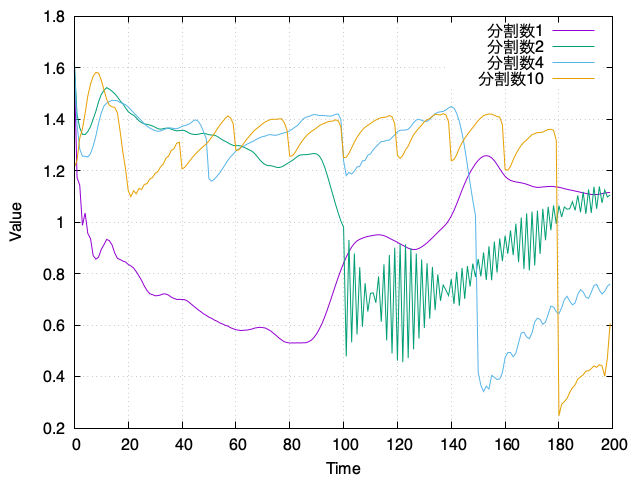
\includegraphics[width=140mm]{images/64error.png}
%\caption{$解像度64^3,障害物なしにおける相対誤差$}
%\label{fig:128error}
%\end{figure}

\begin{figure}[htbp]
\centering
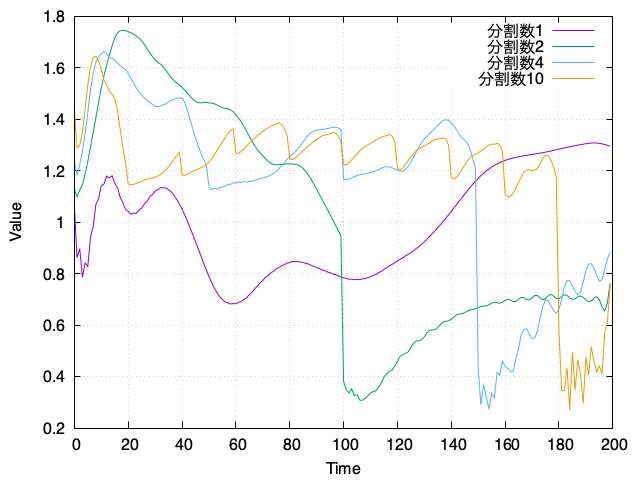
\includegraphics[width=140mm]{images/128error.png}
\caption{$解像度128^3,障害物ありにおける相対誤差$}
\label{fig:128error_obstacle}
\end{figure}

\begin{figure}[htbp]
\centering
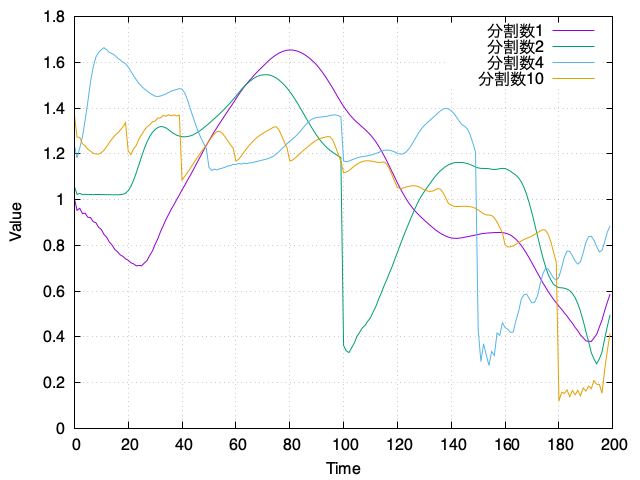
\includegraphics[width=140mm]{images/128error_obstacle.png}
\caption{$解像度128^3,障害物ありにおける相対誤差$}
\label{fig:128error_obstacle}
\end{figure}


%\begin{figure}[htbp]
%\caption{$解像度64^3$,分割数10における,流速の分布と誤差}
%\label{fig:n128_vel}
%\centering
%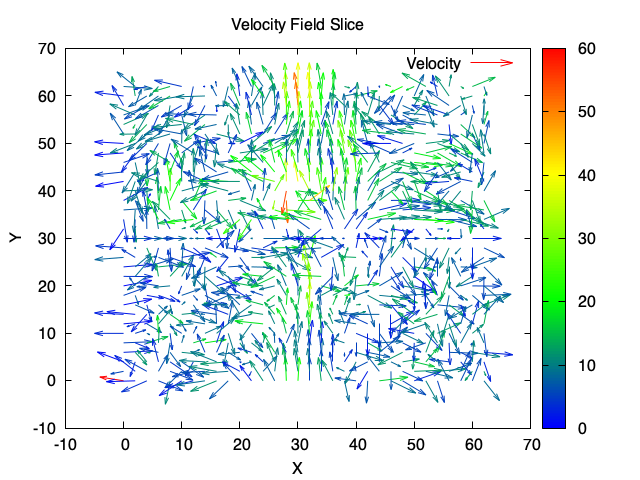
\includegraphics[width=140mm]{images/velocity_plot_100.png}
%\subcaption{100フレーム目}
%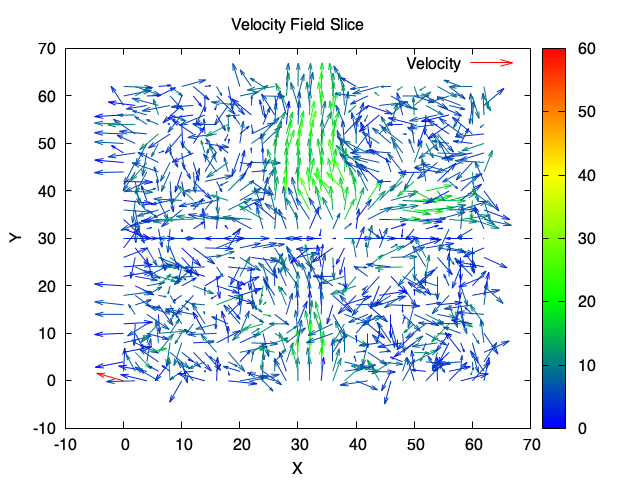
\includegraphics[width=140mm]{images/velocity_plot_101.png}
%\subcaption{101フレーム目}
%\end{figure}

\begin{figure}[htbp]
\caption{$解像度128^3$,分割数2,障害物ありのシミュレーションにおける,流速の分布と誤差}
\label{fig:n128_obst_vel}
\centering
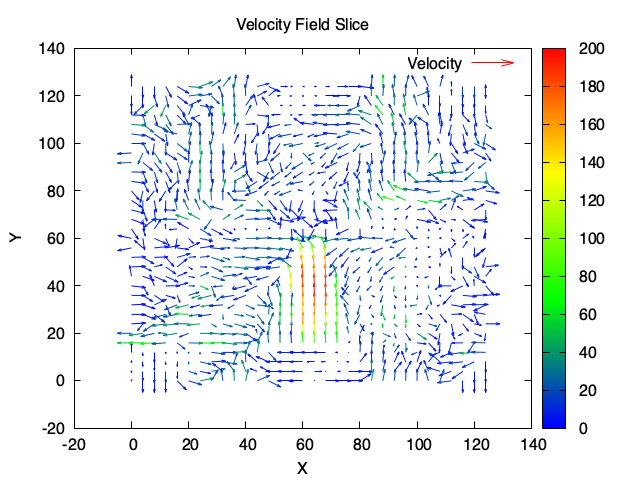
\includegraphics[width=140mm]{images/velocity_plot_100_obst.png}
\subcaption{100フレーム目}
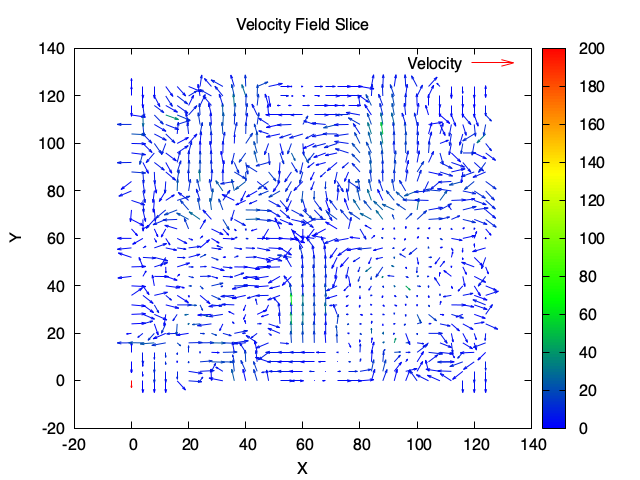
\includegraphics[width=140mm]{images/velocity_plot_101_obst.png}
\subcaption{101フレーム目}
\end{figure}

%また,本手法の課題として,実験に用いるシミュレーションデータの質に左右される.シミュレーションデータ内で計算が発散していない場合でも,部分空間に射影することで計算が発散し,意味のある結果が得られない場合がある.以下は外力項のパラメータを高く設定した例である.

%\begin{figure}[htbp]
%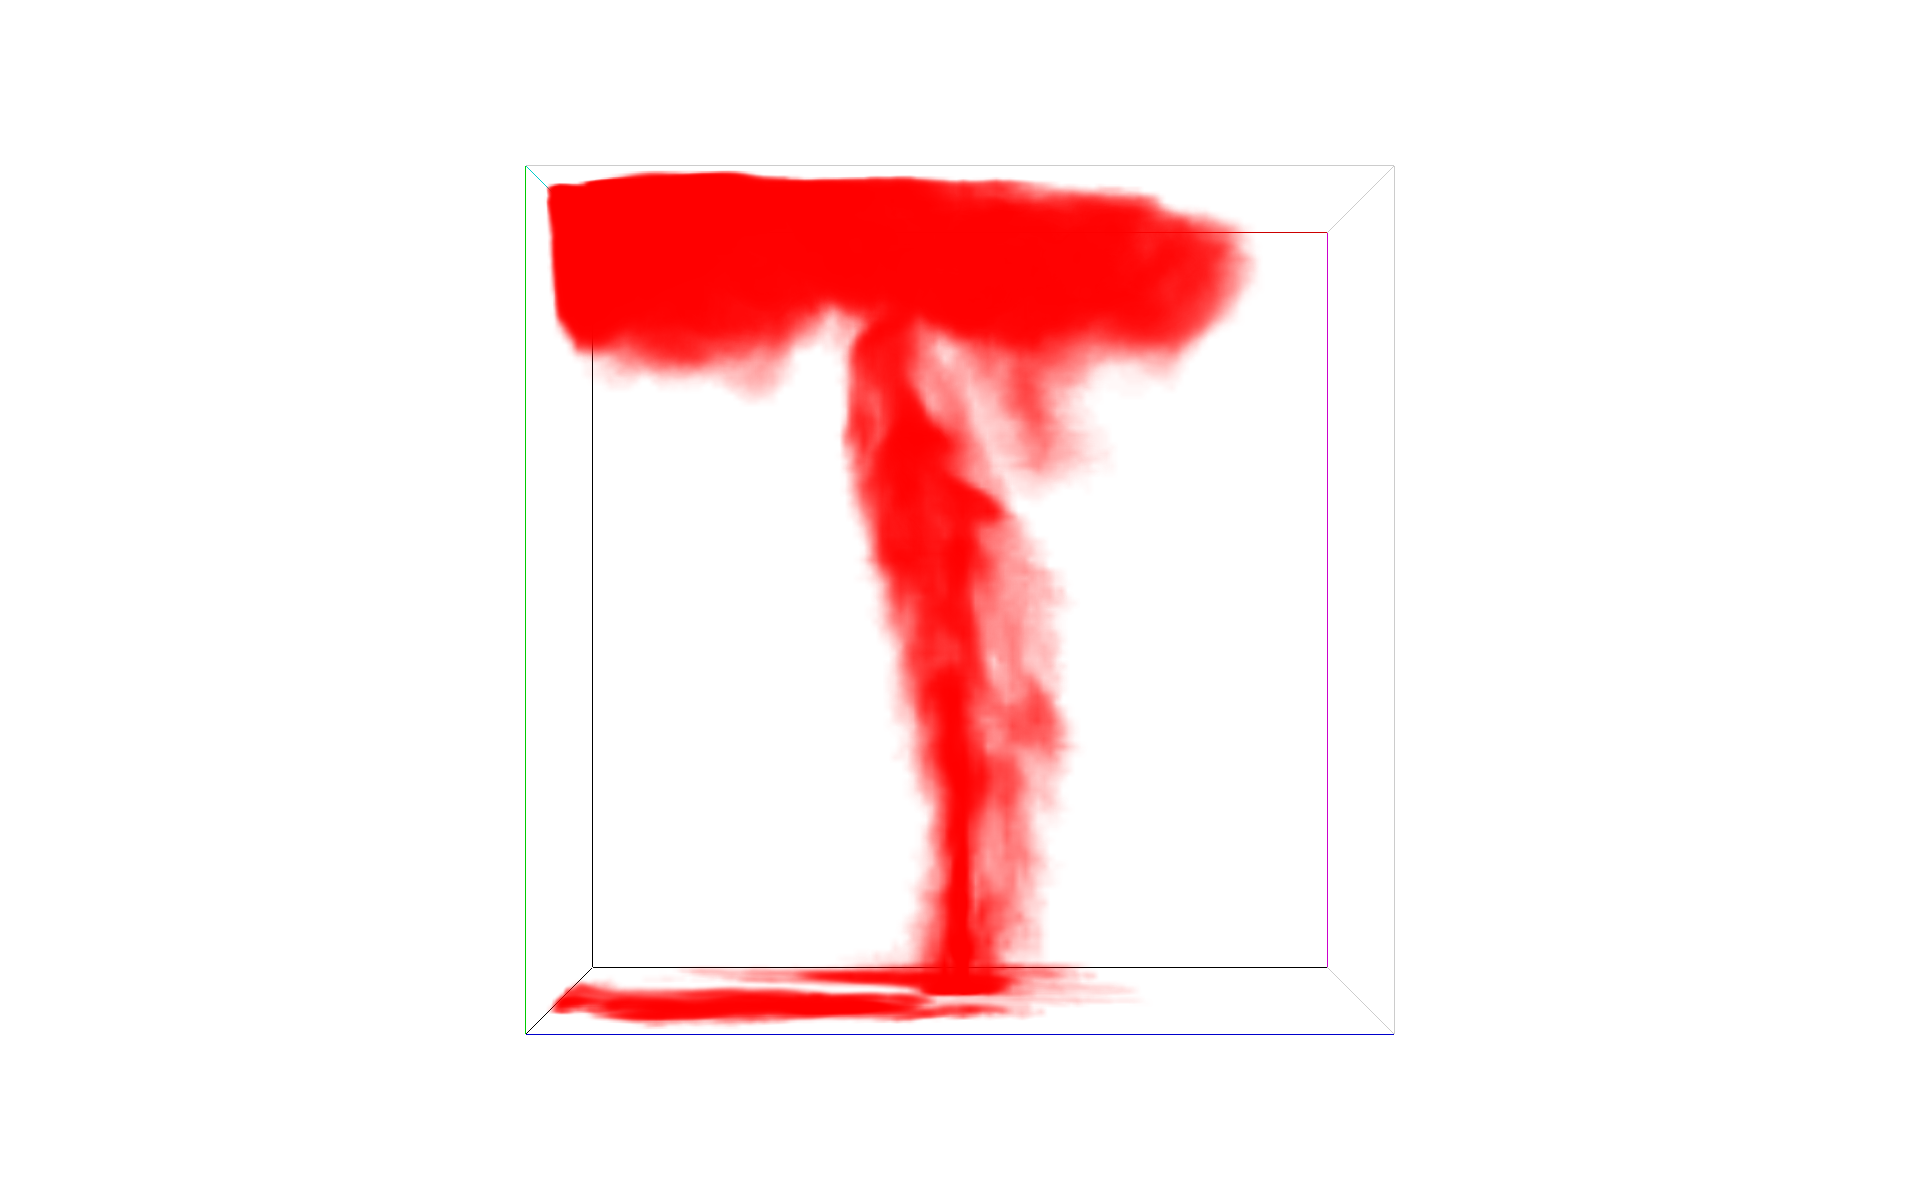
\includegraphics[width=140mm]{images/n128_f99_truth.png}
%\caption{$解像度128^3,ground truth,99フレーム目$}
%\label{fig:n128_f99_div4}
%\end{figure}

\begin{figure}[htbp]
\caption{$解像度128^3,障害物なし,100フレーム目$}
\label{fig:n128_f99}
\centering
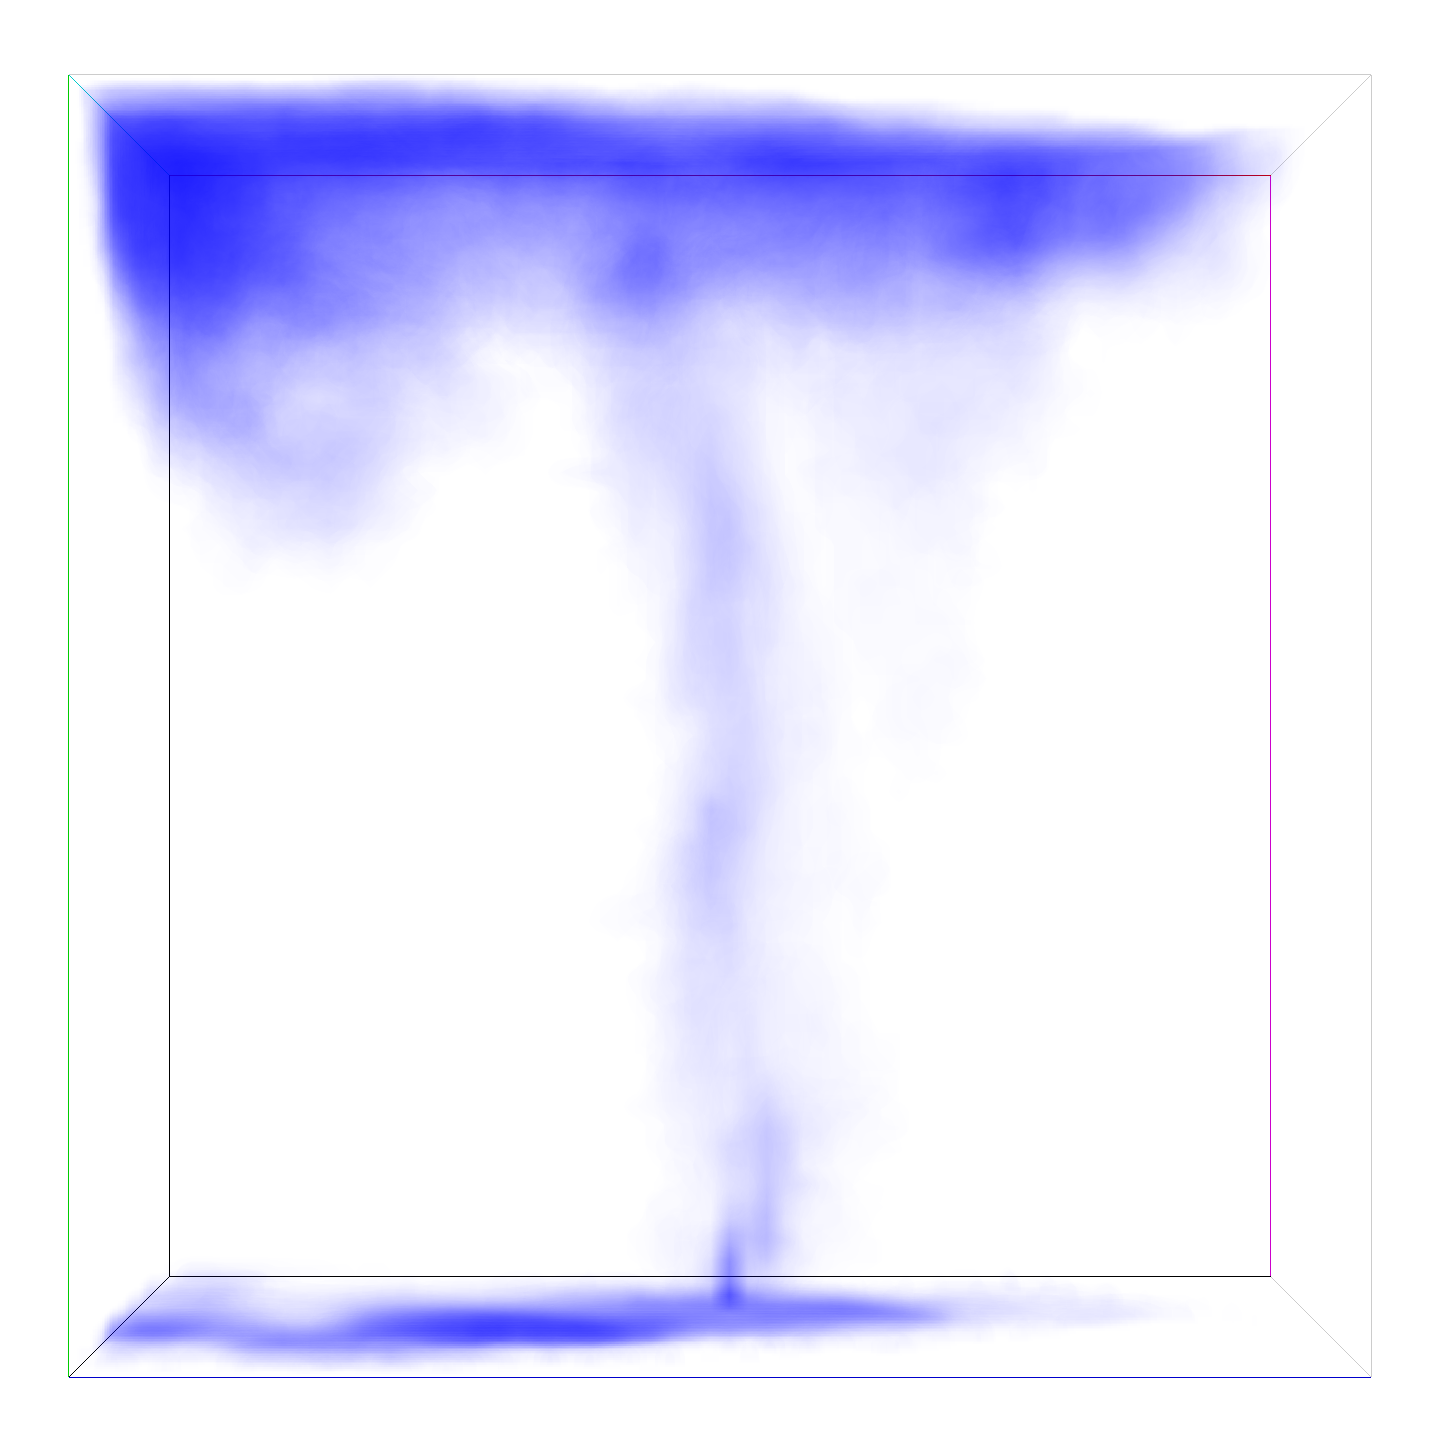
\includegraphics[width=65mm]{images/n64_origin_f99.png}
\subcaption{gruound truth}

\begin{tabular}{cc}
\begin{minipage}[b]{0.45\linewidth}
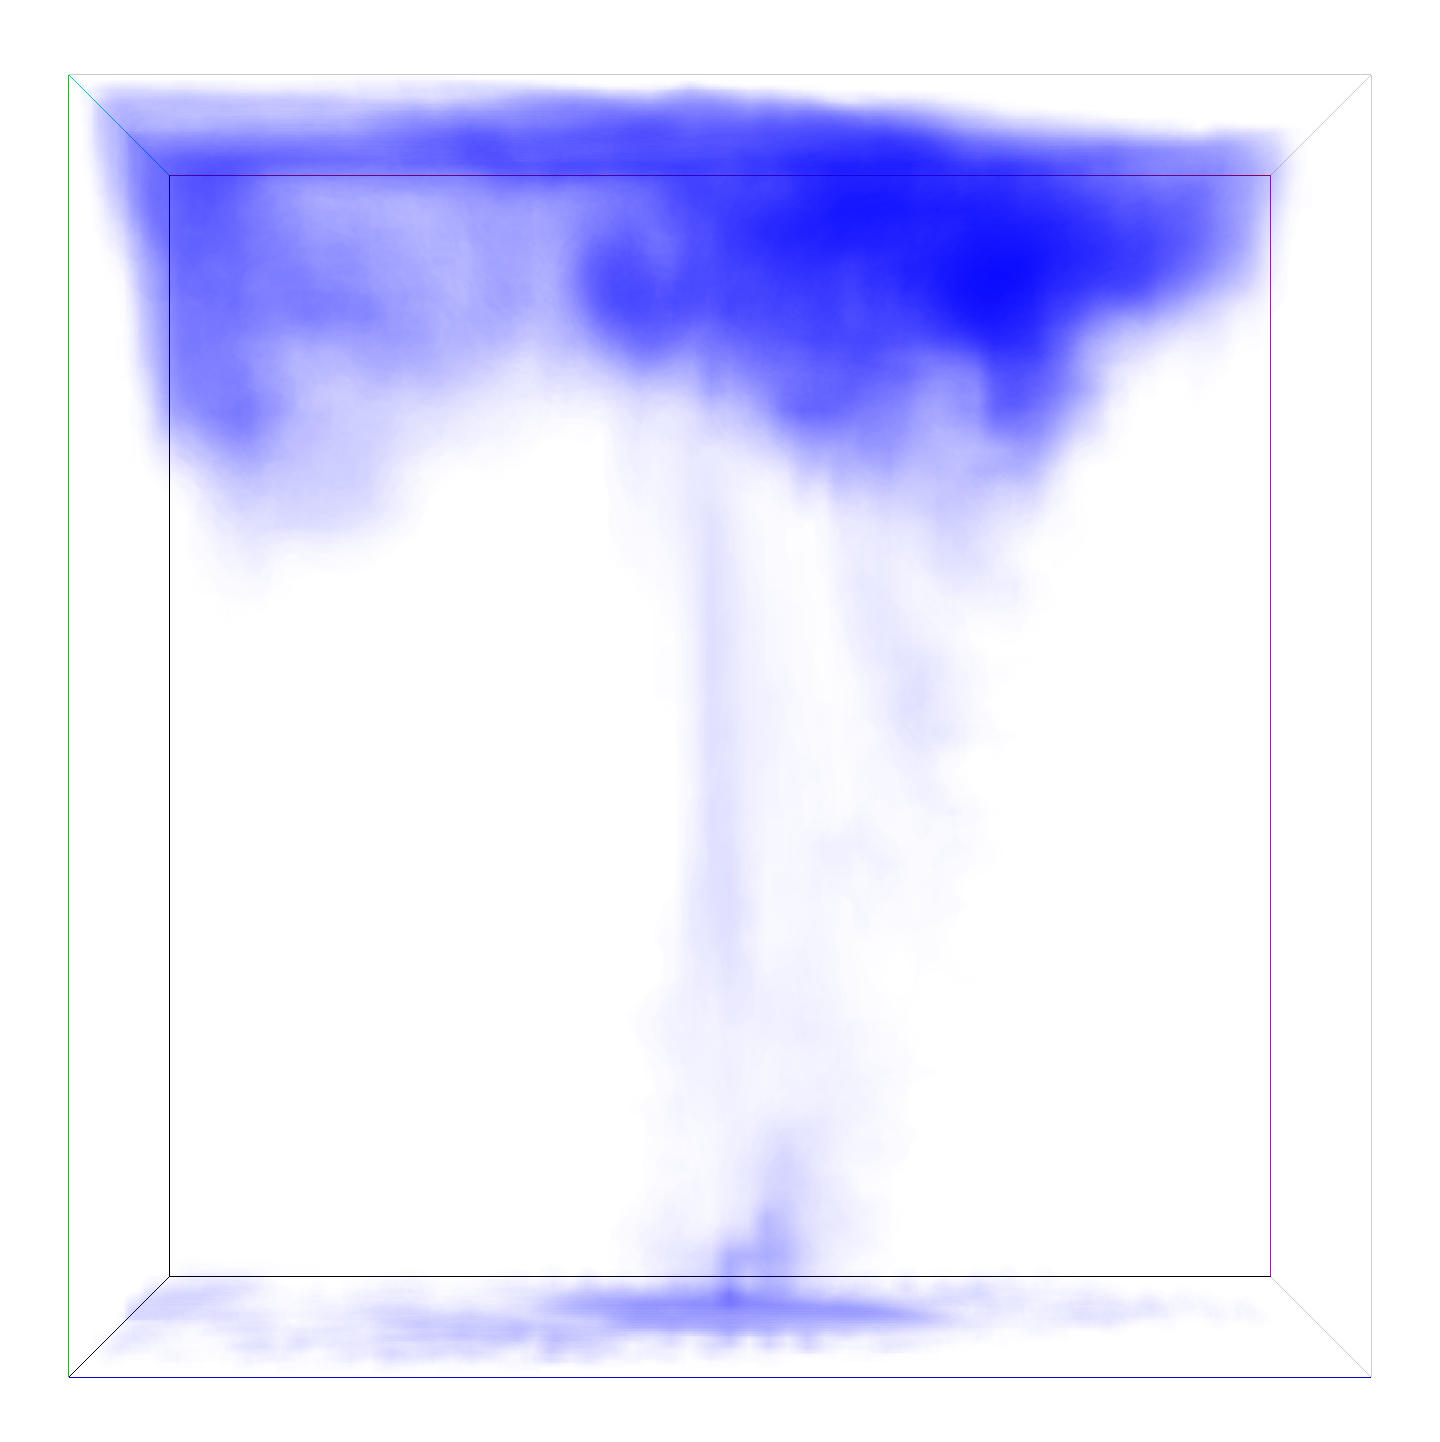
\includegraphics[width=65mm]{images/n64_div1_f99.png}
\subcaption{分割数1}
\end{minipage}

\begin{minipage}[b]{0.45\linewidth}
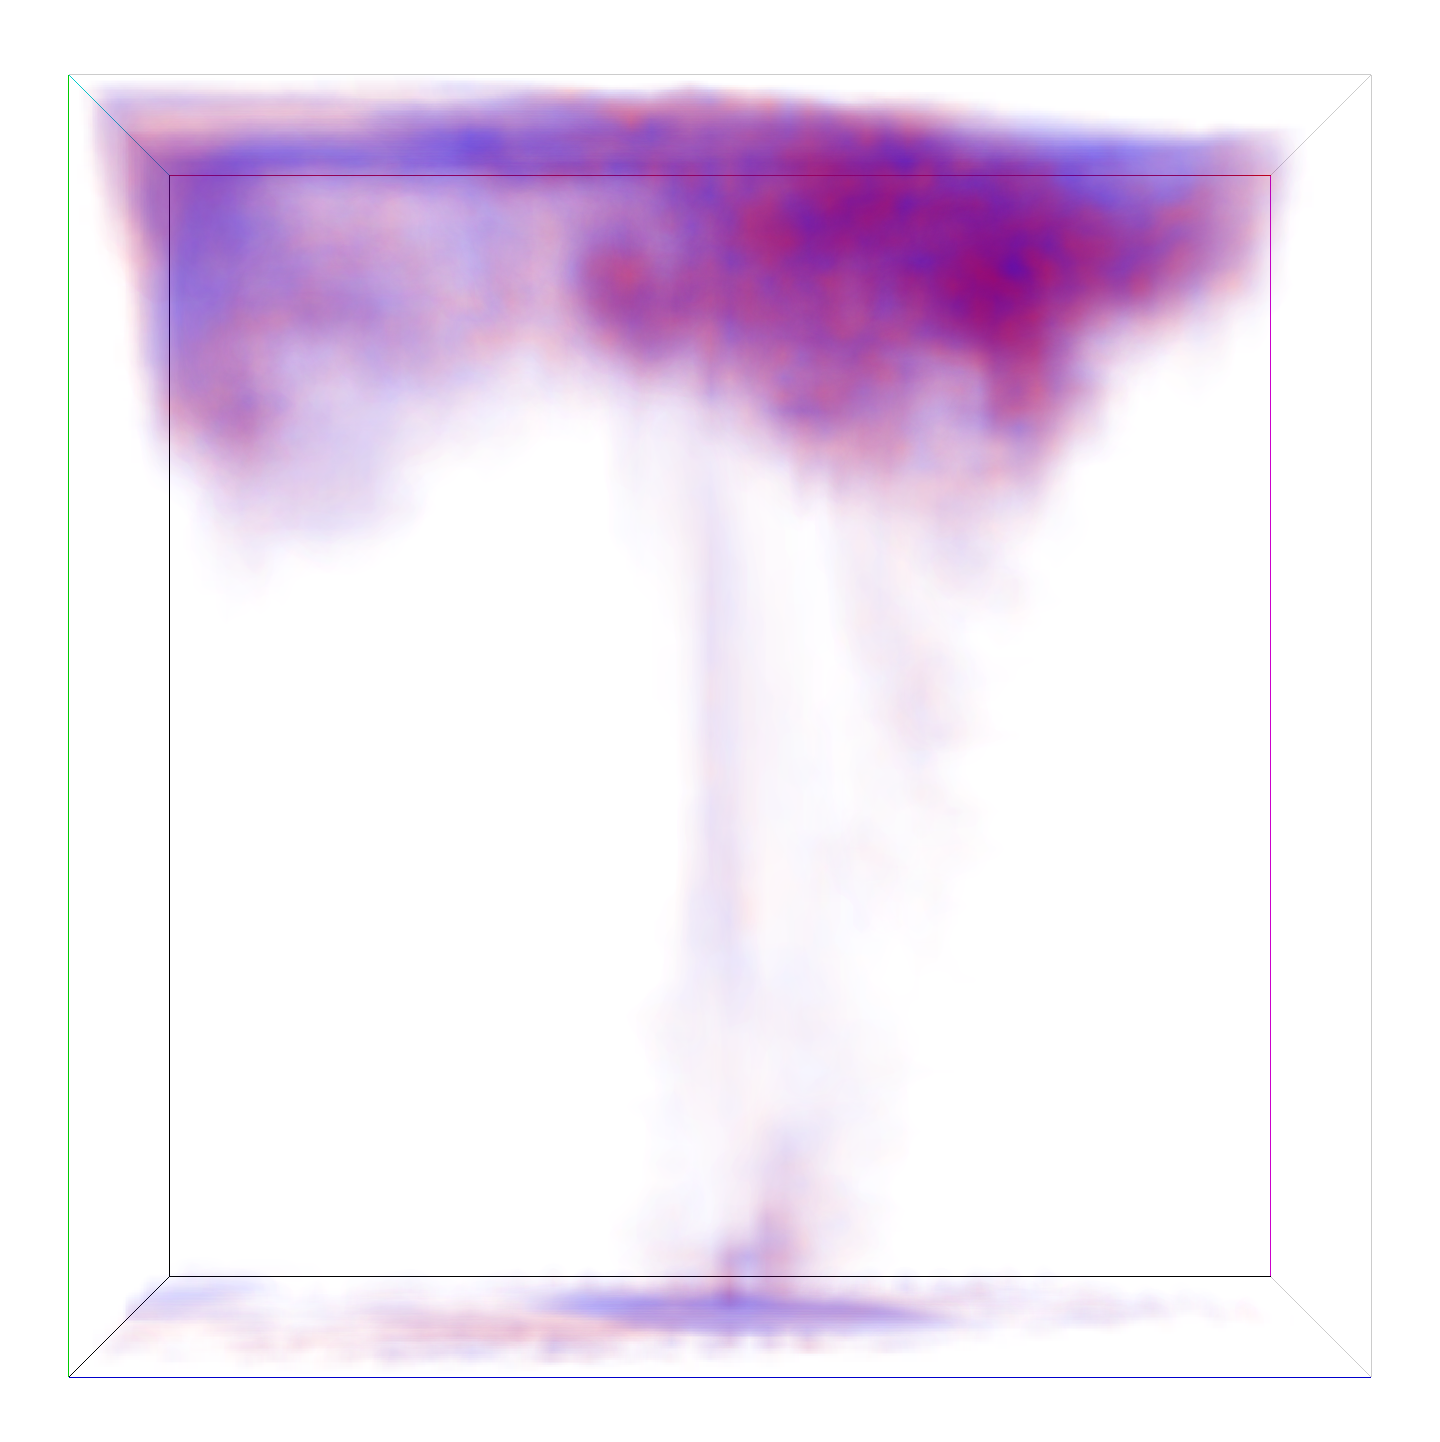
\includegraphics[width=65mm]{images/n64_div1_f99_color.png}
\subcaption{分割数1,誤差による色付け}
\end{minipage}
\\
\begin{minipage}[b]{0.45\linewidth}
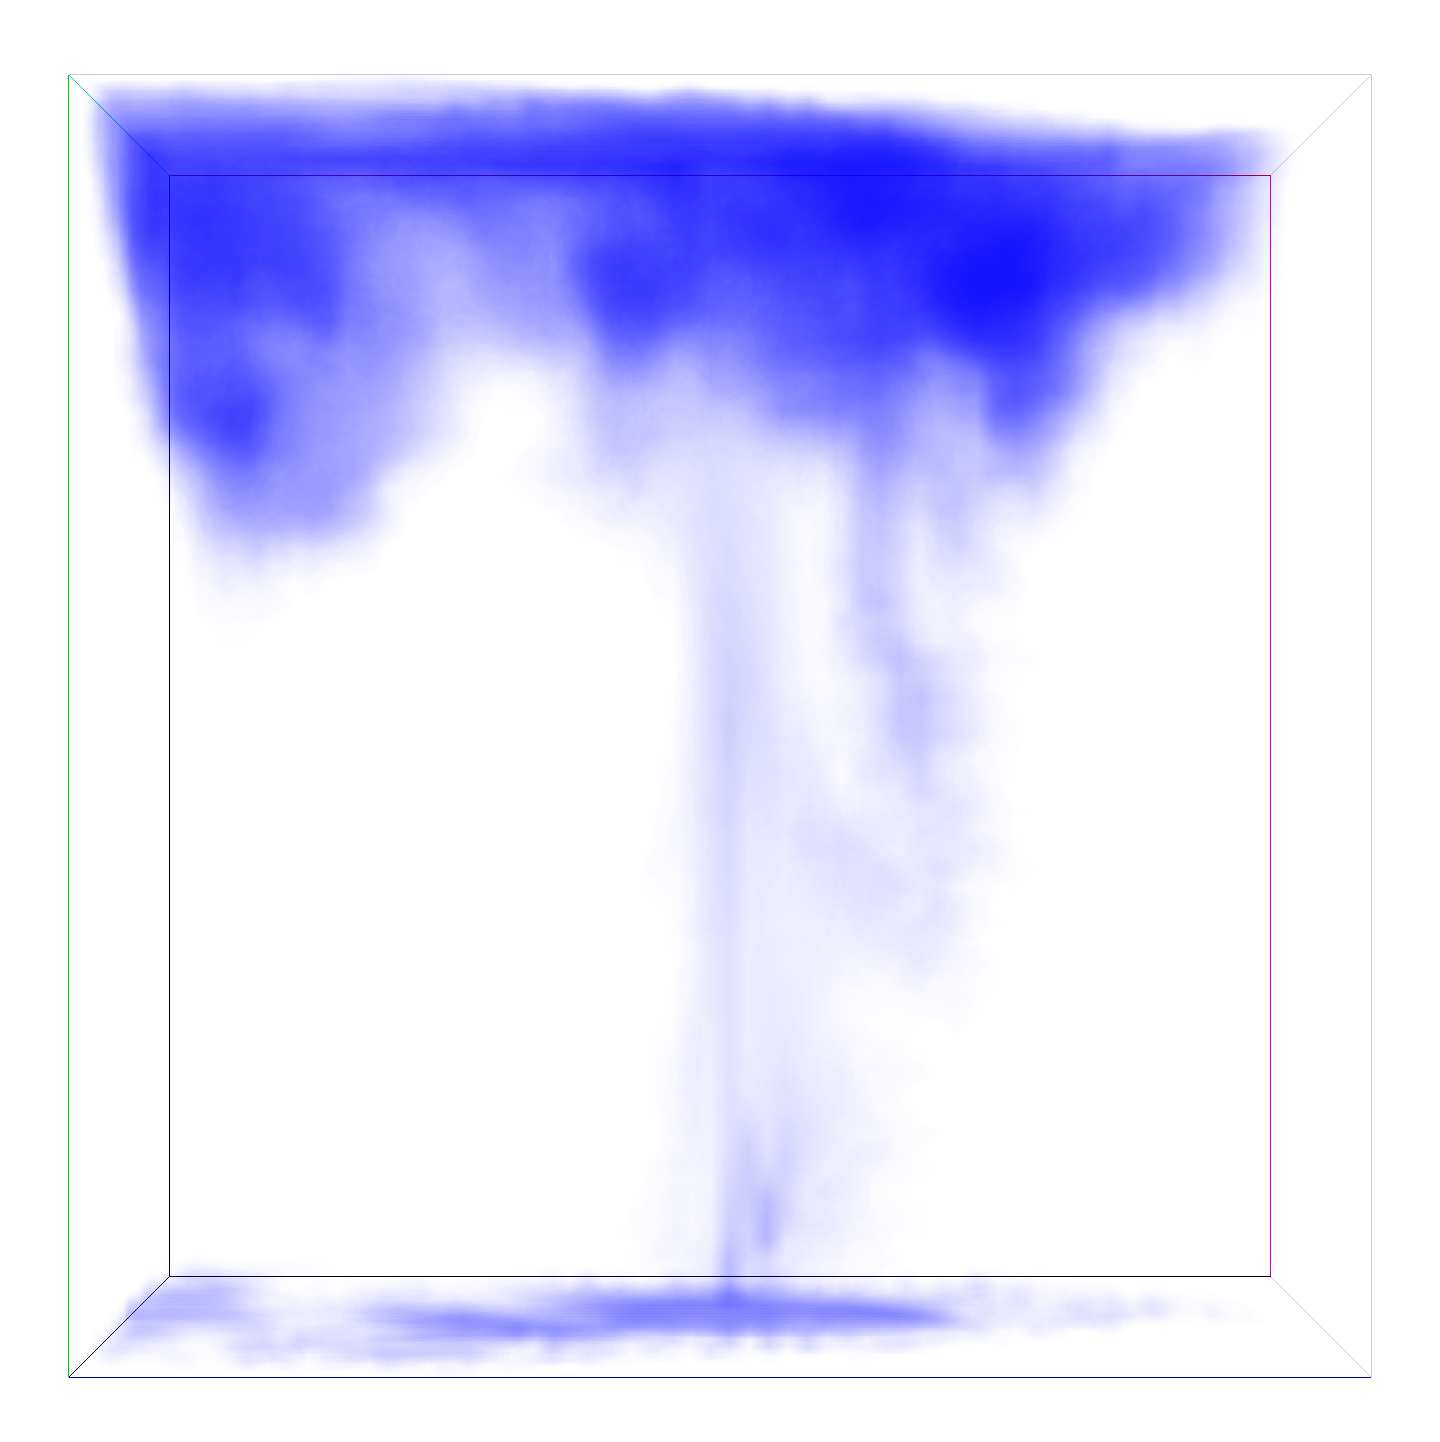
\includegraphics[width=65mm]{images/n64_div2_f99.png}
\subcaption{分割数2}
\end{minipage}

\begin{minipage}[b]{0.45\linewidth}
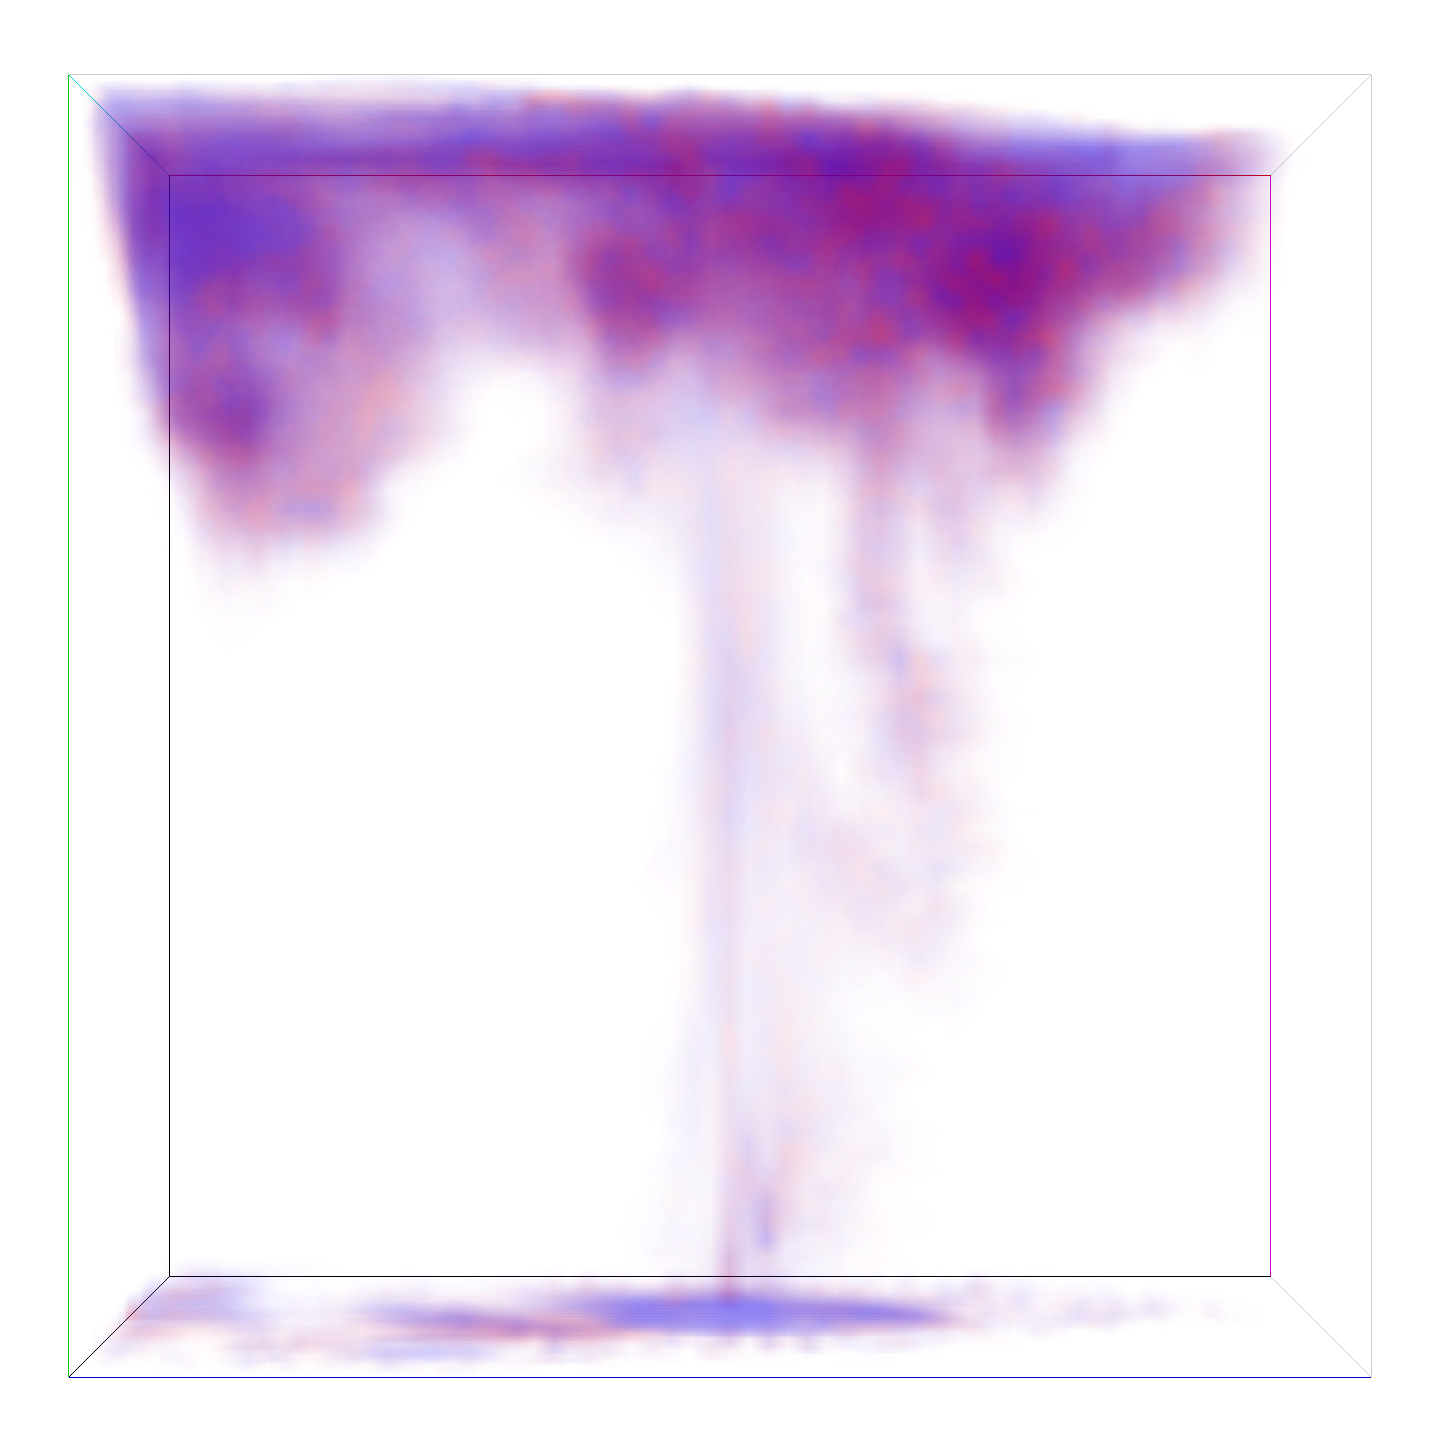
\includegraphics[width=65mm]{images/n64_div2_f99_color.png}
\subcaption{分割数2,誤差による色付け}
\end{minipage}
\end{tabular}
\end{figure}

\begin{figure}[htbp]
\caption{$解像度128^3,障害物なし,101フレーム目$}
\label{fig:n128_f100}
\centering
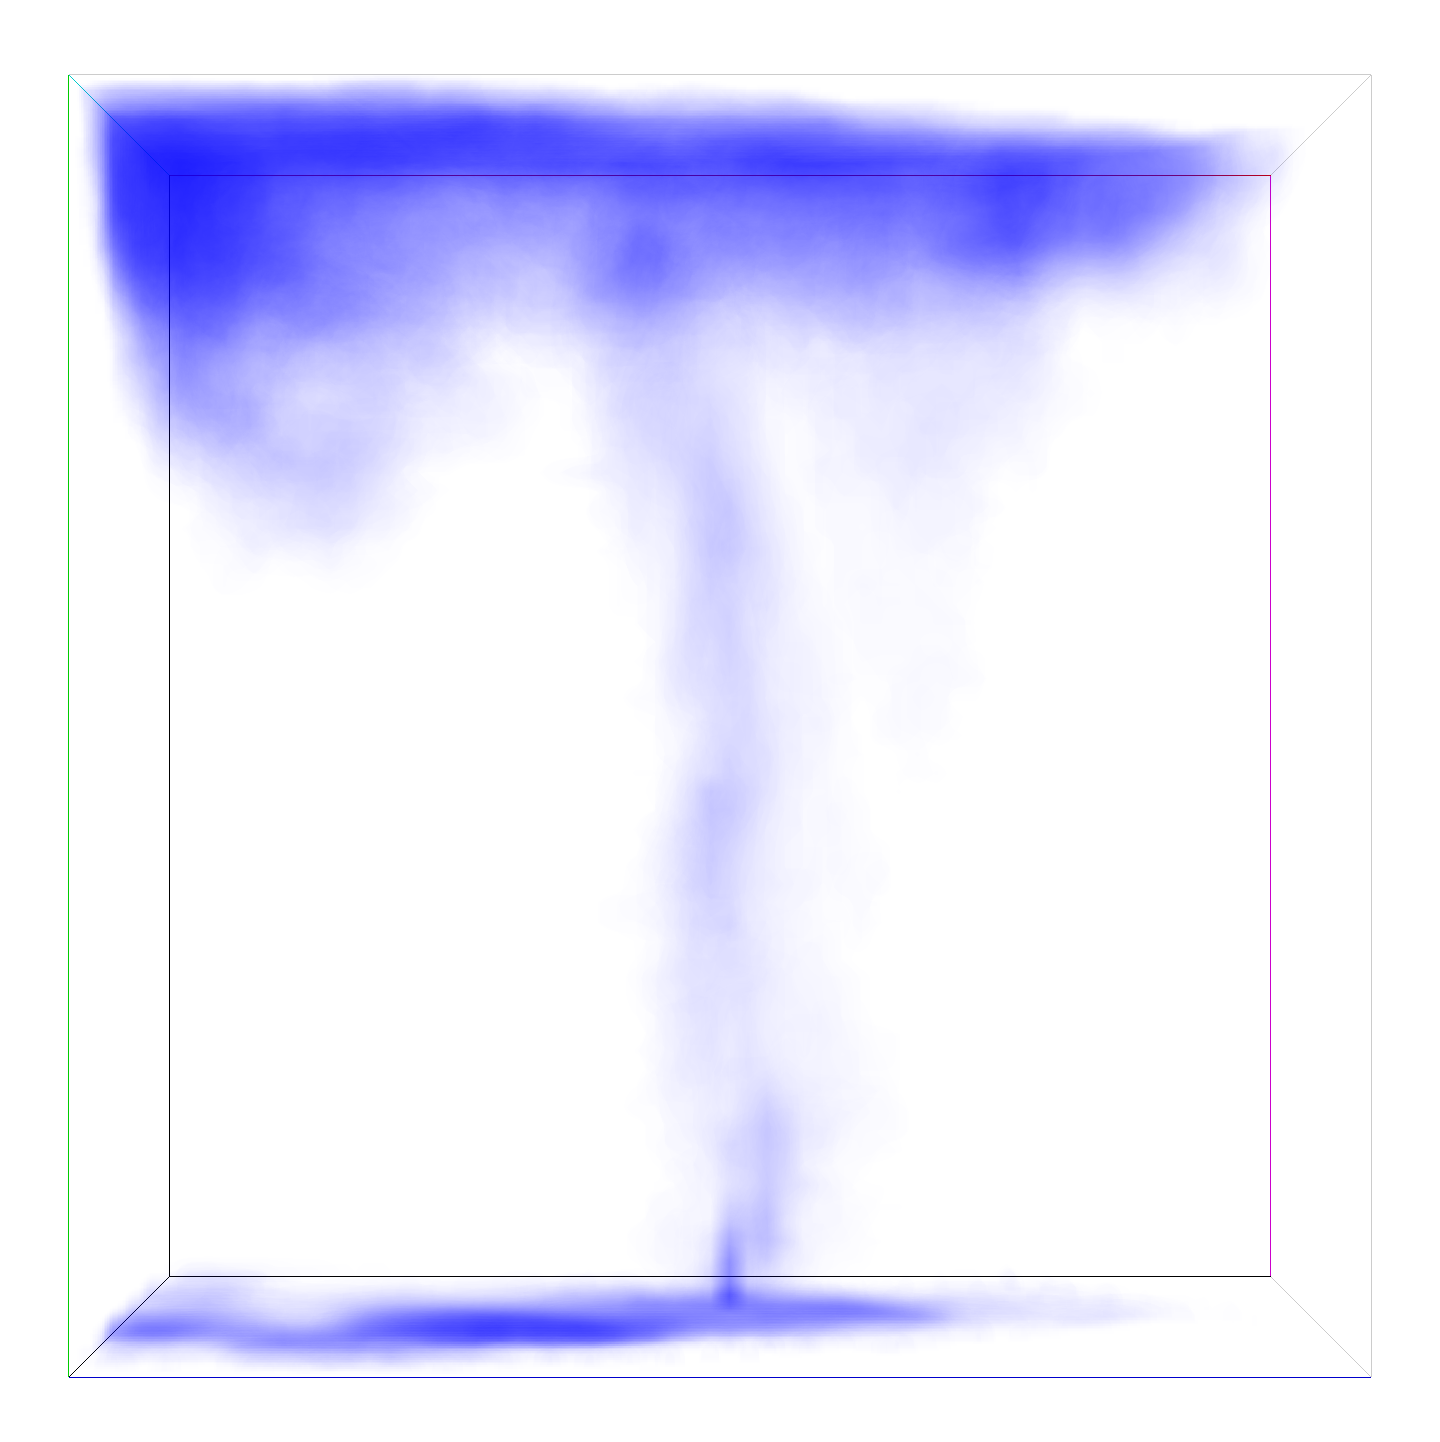
\includegraphics[width=65mm]{images/n64_origin_f100.png}
\subcaption{gruound truth}

\begin{tabular}{cc}
\begin{minipage}[b]{0.45\linewidth}
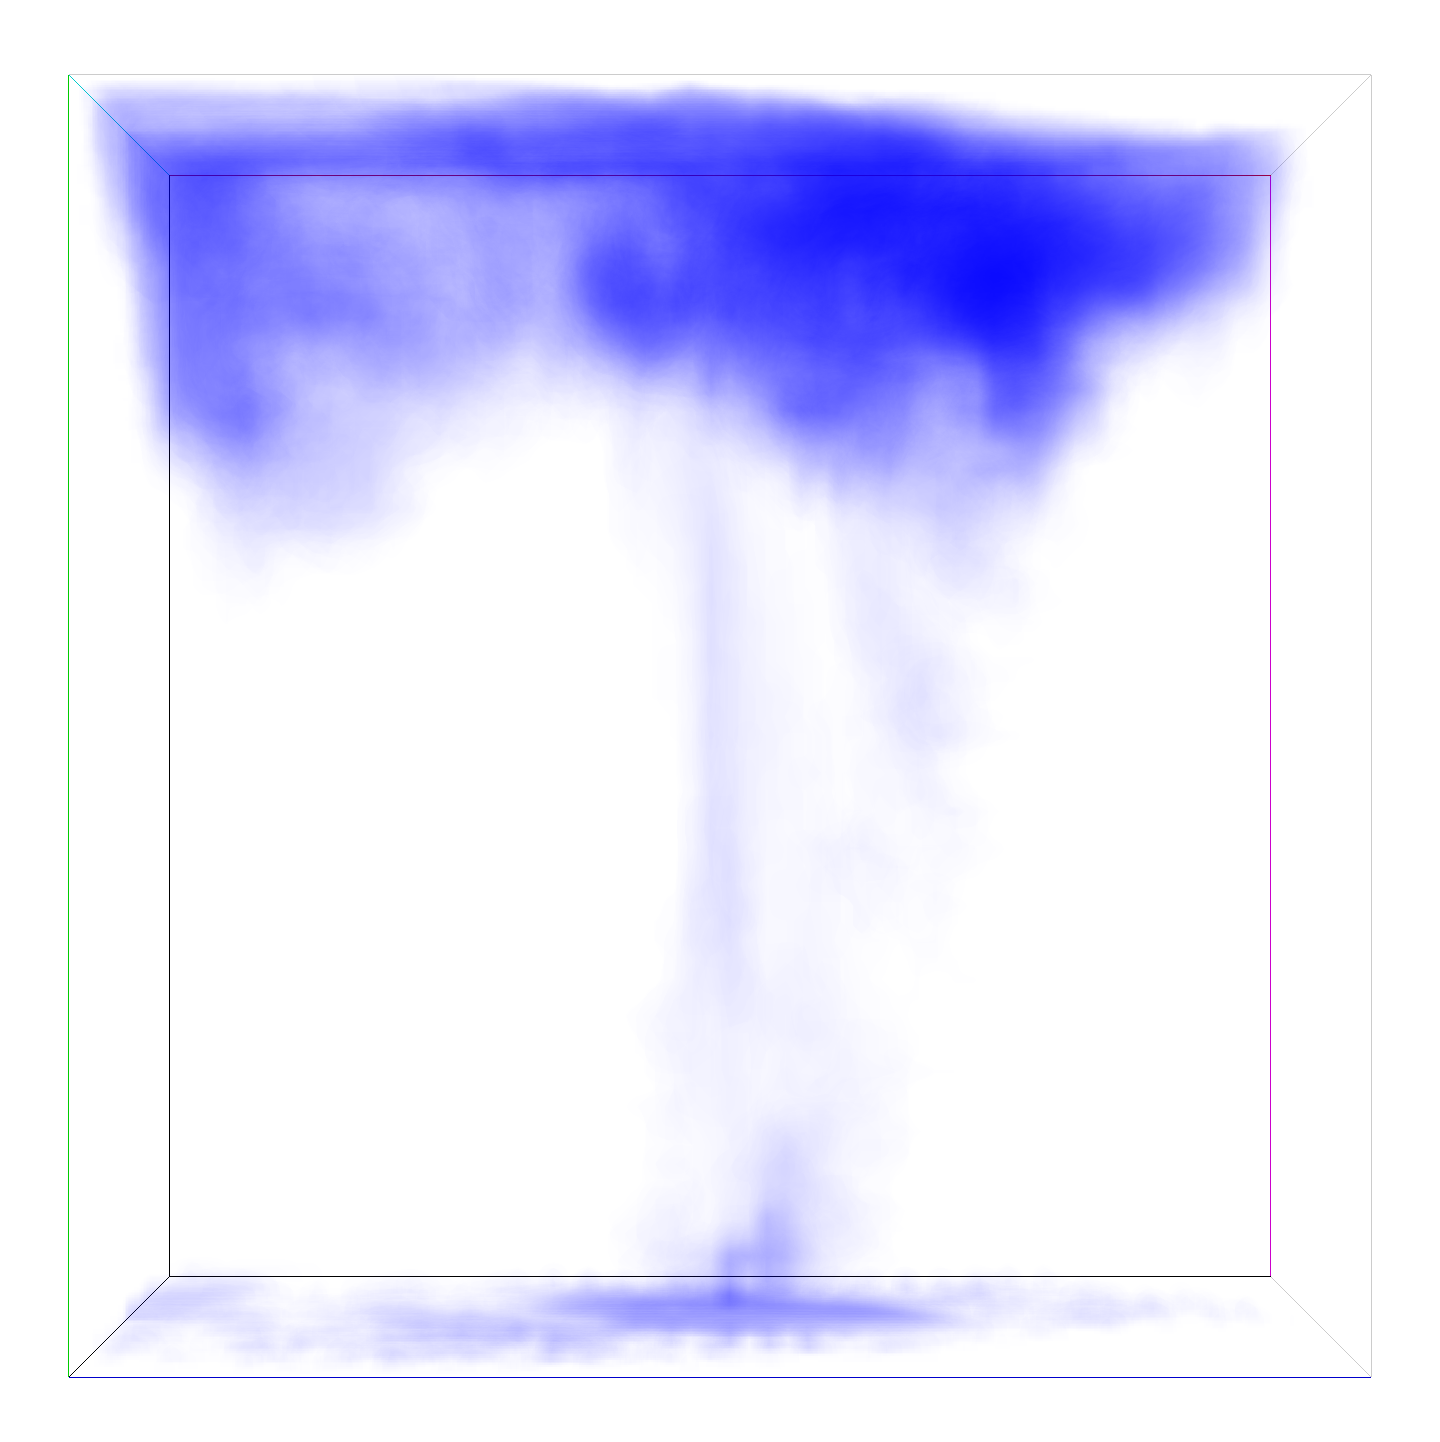
\includegraphics[width=65mm]{images/n64_div1_f100.png}
\subcaption{分割数1}
\end{minipage}

\begin{minipage}[b]{0.45\linewidth}
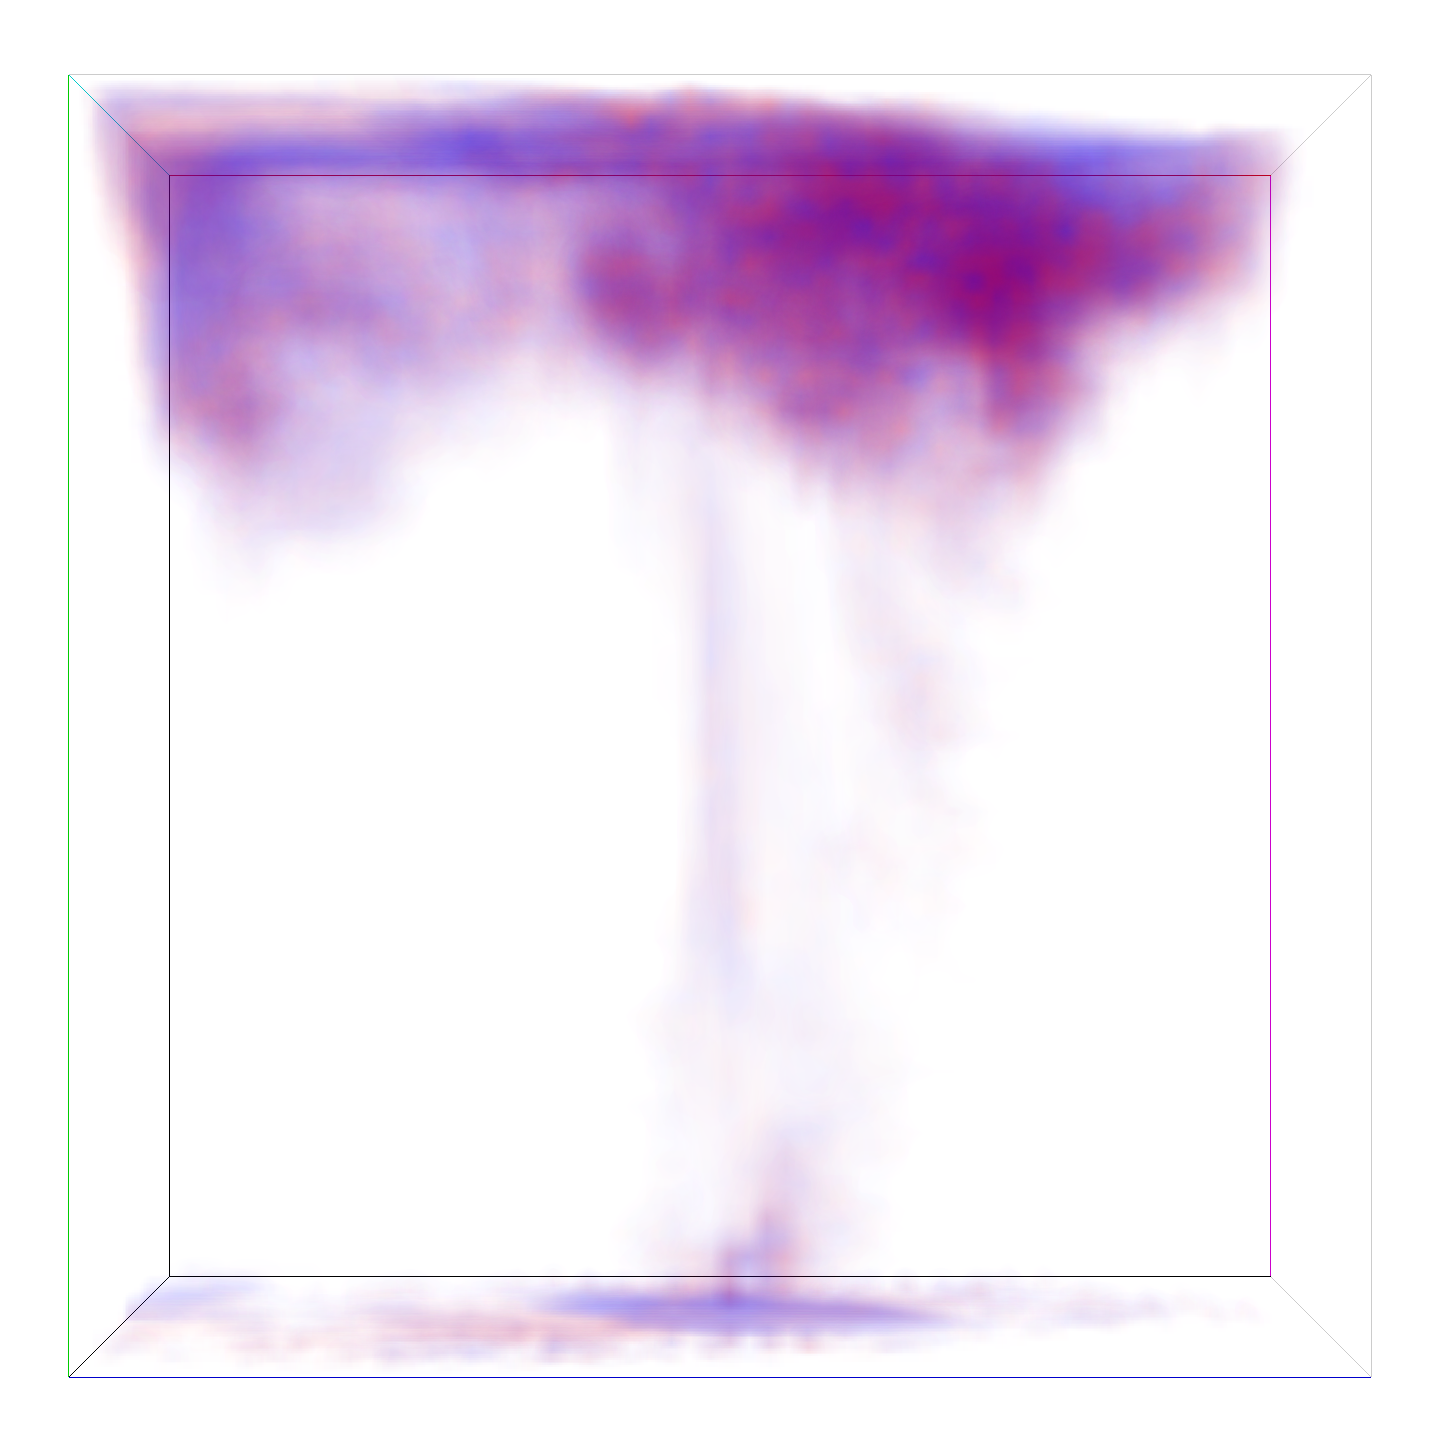
\includegraphics[width=65mm]{images/n64_div1_f100_color.png}
\subcaption{分割数1,誤差による色付け}
\end{minipage}
\\
\begin{minipage}[b]{0.45\linewidth}
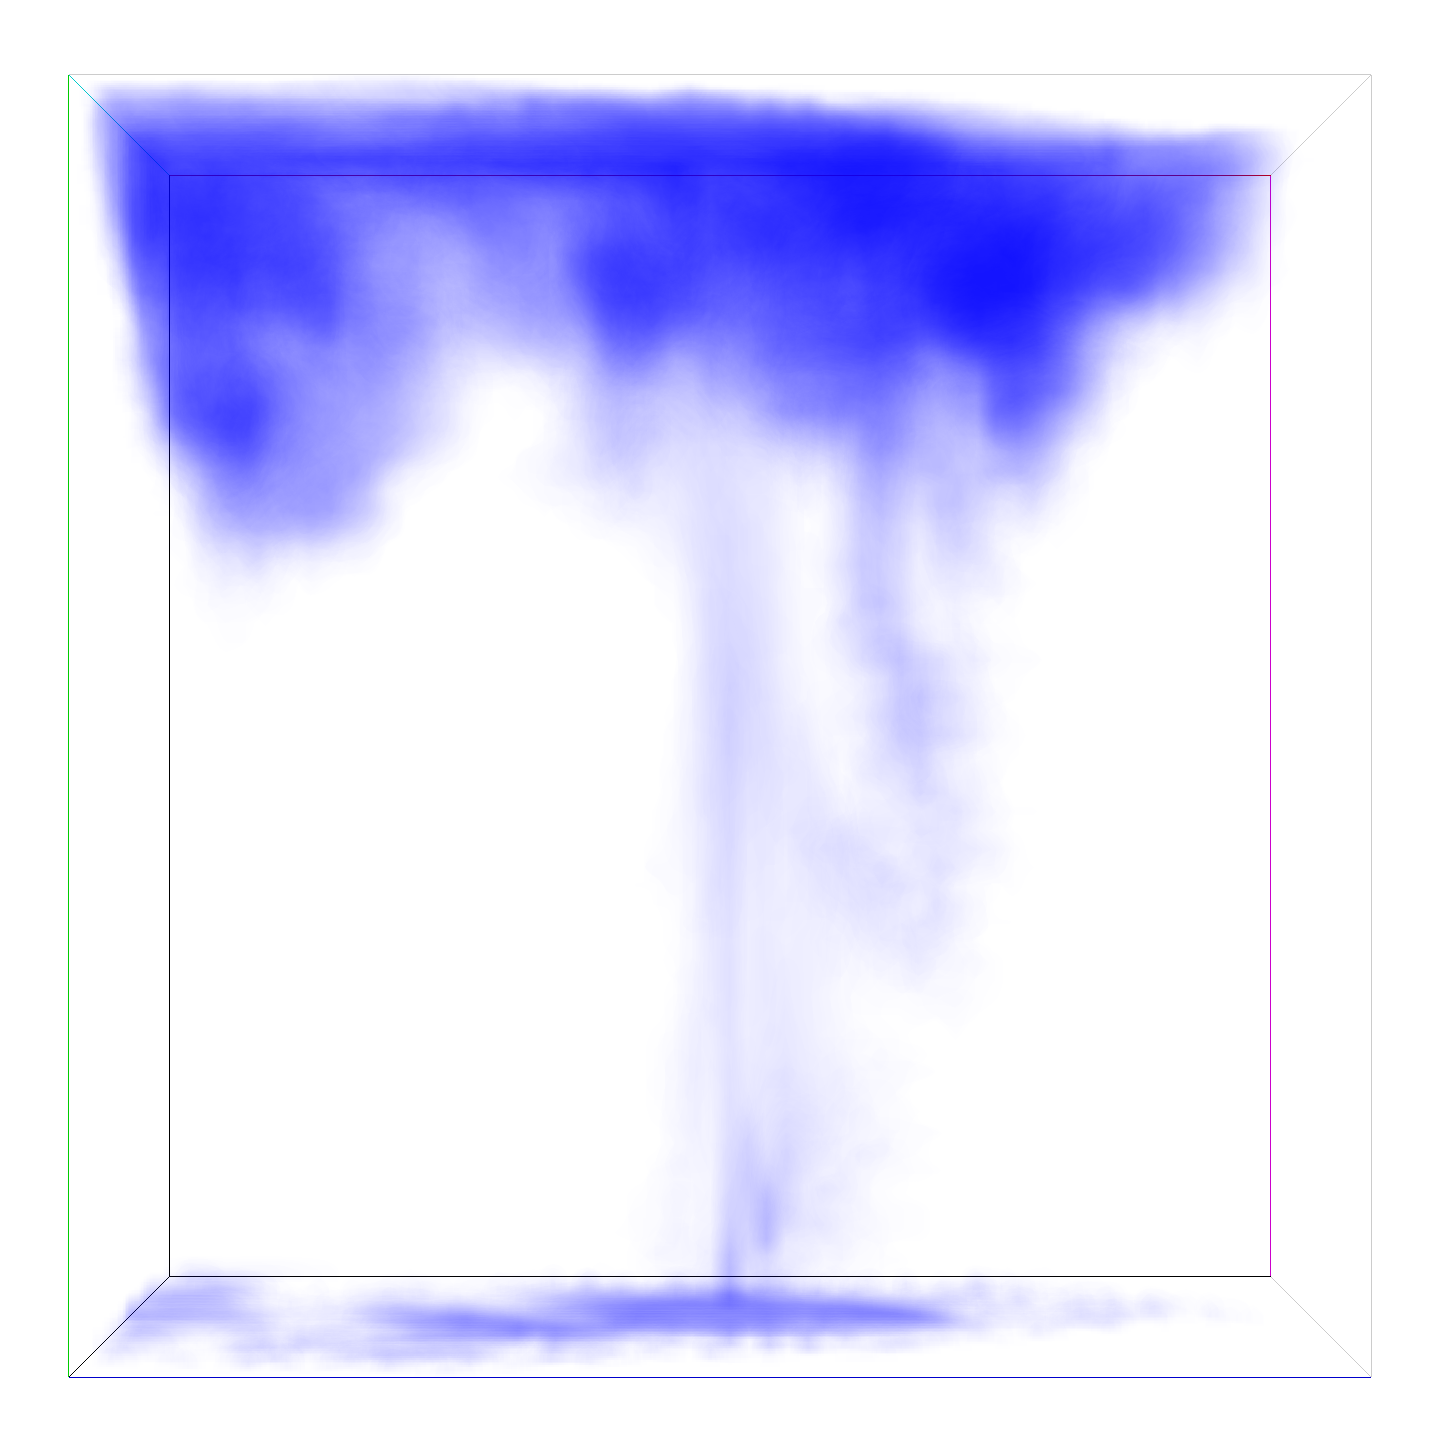
\includegraphics[width=65mm]{images/n64_div2_f100.png}
\subcaption{分割数2}
\end{minipage}

\begin{minipage}[b]{0.45\linewidth}
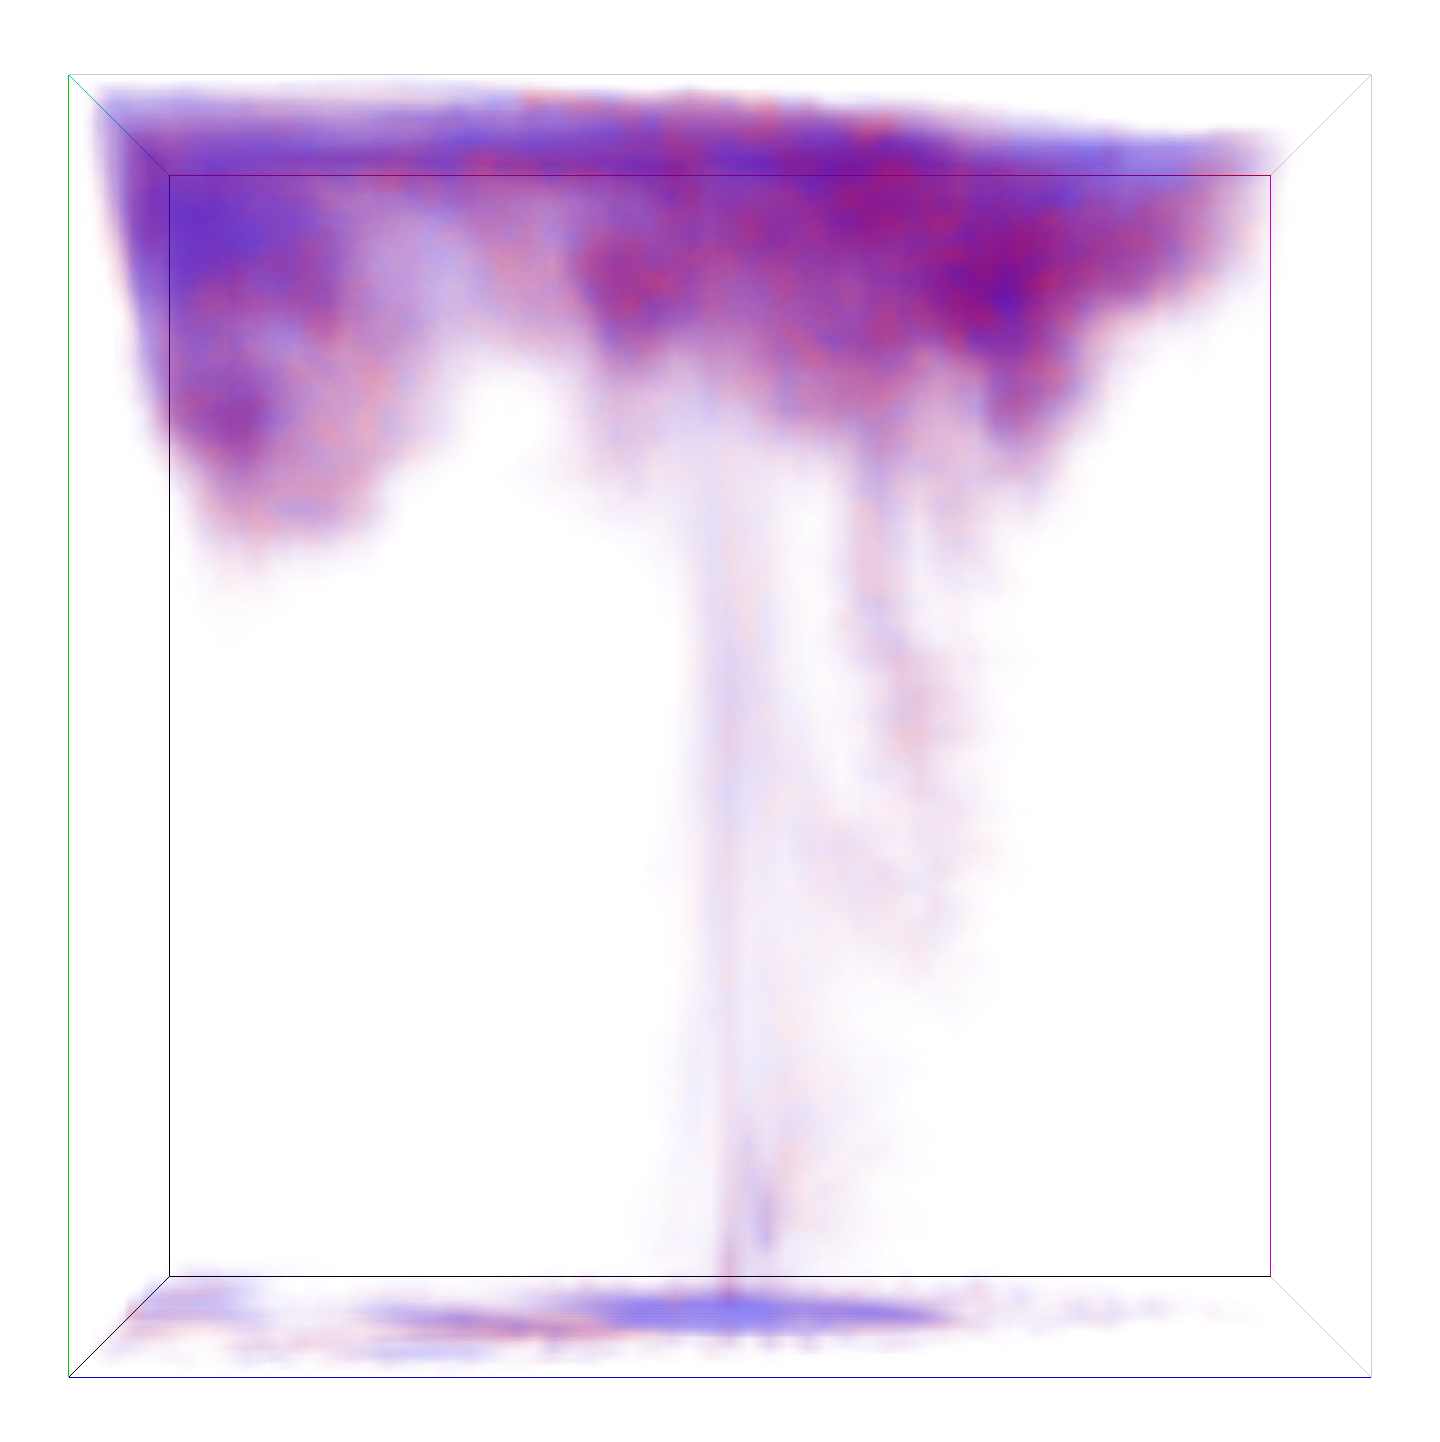
\includegraphics[width=65mm]{images/n64_div2_f100_color.png}
\subcaption{分割数2,誤差による色付け}
\end{minipage}
\end{tabular}
\end{figure}

%\begin{figure}[htbp]
%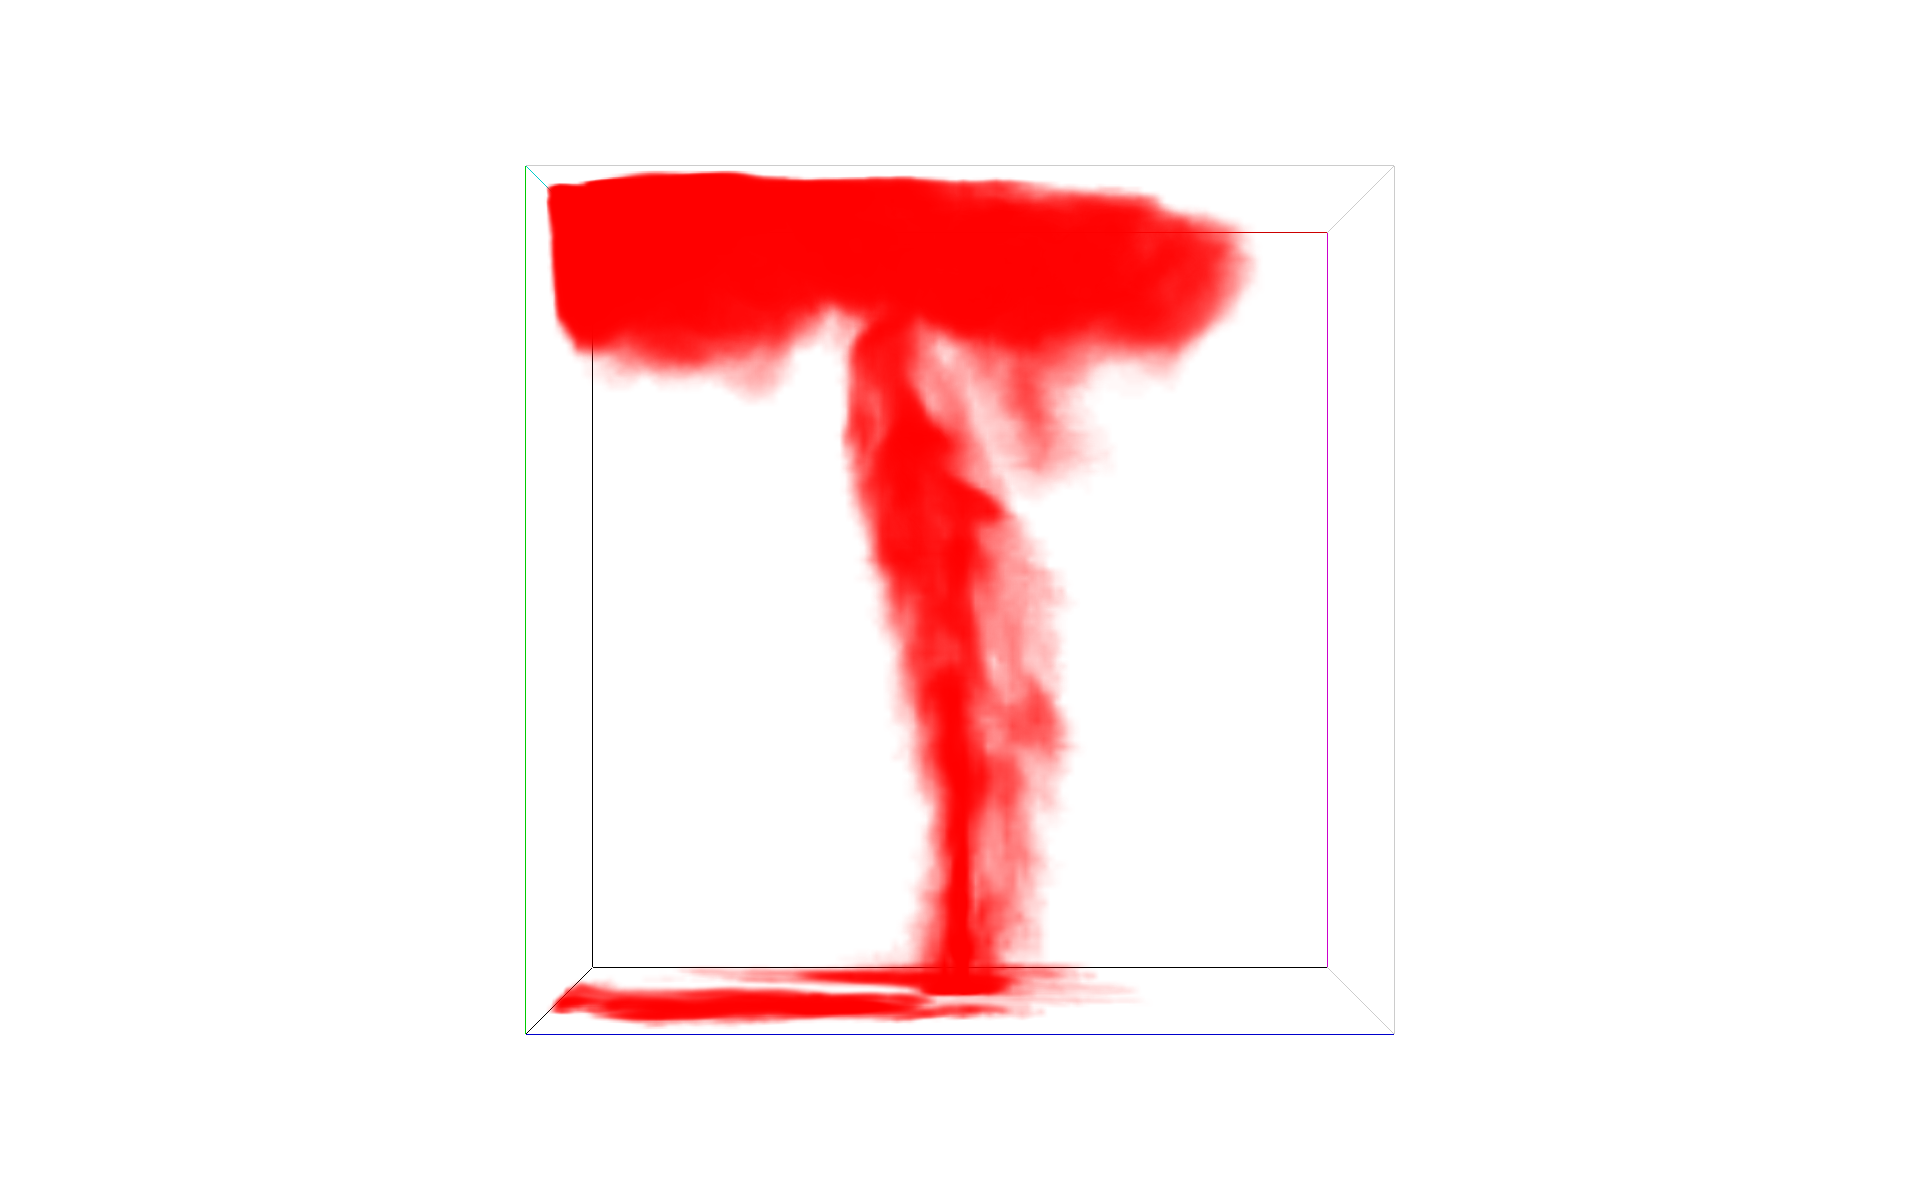
\includegraphics[width=140mm]{images/n128_f99_truth.png}
%\caption{$解像度128^3,ground truth,99フレーム目$}
%\label{fig:n128_f99_div4}
%\end{figure}

\begin{figure}[htbp]
\caption{$解像度128^3,障害物あり,100フレーム目$}
\label{fig:n128_f99_obstacle}
\centering
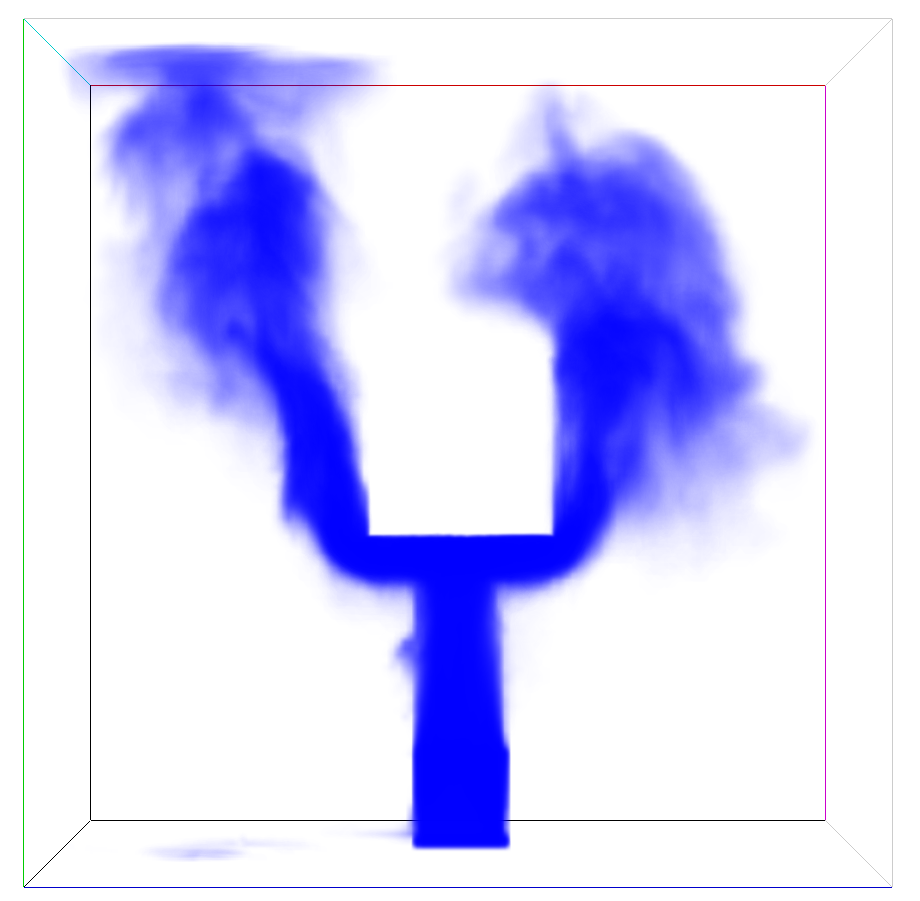
\includegraphics[width=65mm]{images/n128_origin_f99_obstacle.png}
\subcaption{gruound truth}

\begin{tabular}{cc}
\begin{minipage}[b]{0.45\linewidth}
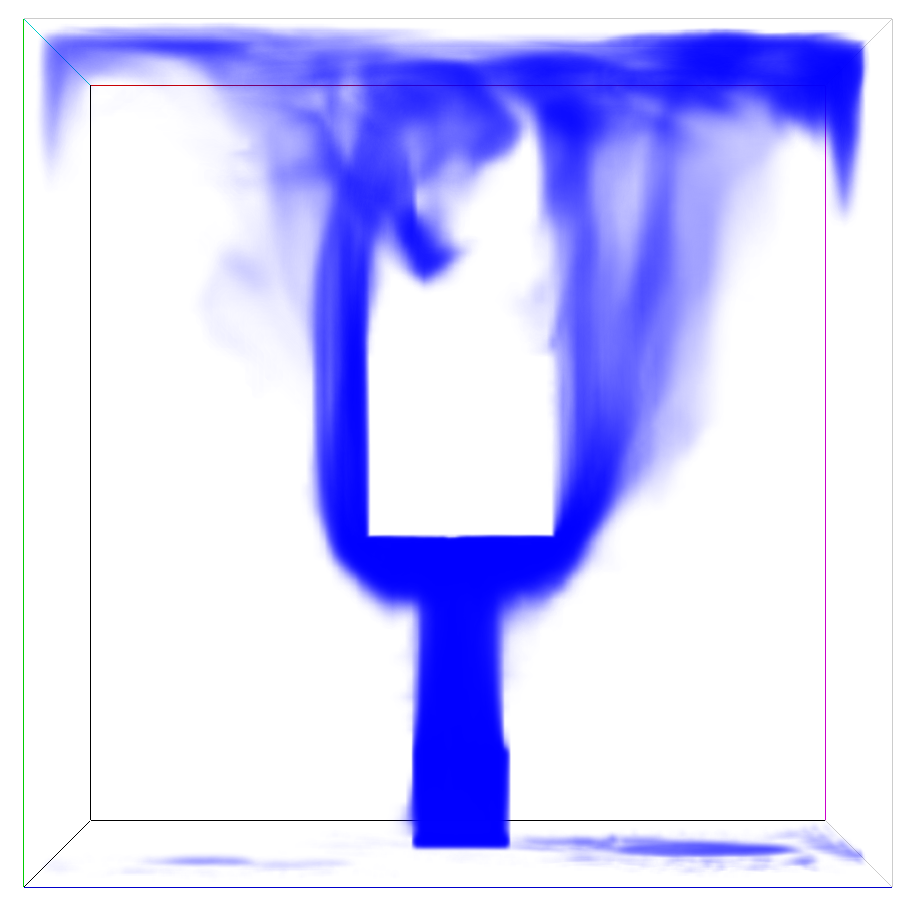
\includegraphics[width=65mm]{images/n128_dev1_f99_obstacle.png}
\subcaption{分割数1}
\end{minipage}

\begin{minipage}[b]{0.45\linewidth}
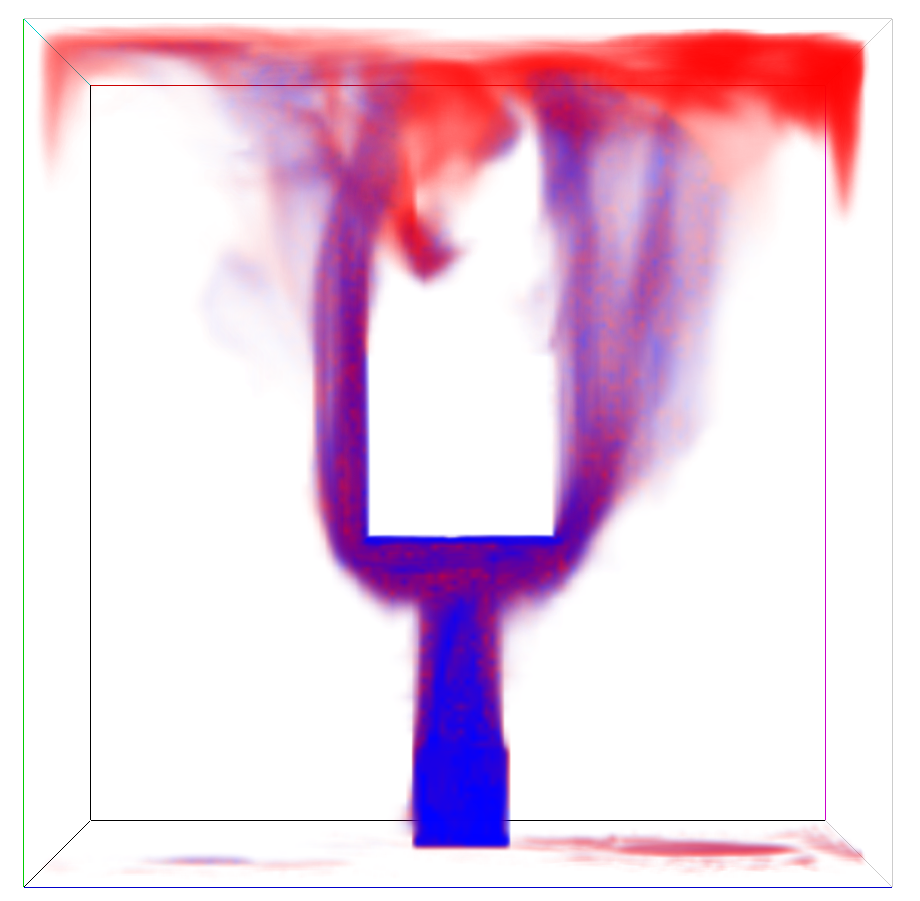
\includegraphics[width=65mm]{images/n128_dev1_f99_obstacle_color.png}
\subcaption{分割数1,誤差による色付け}
\end{minipage}
\\
\begin{minipage}[b]{0.45\linewidth}
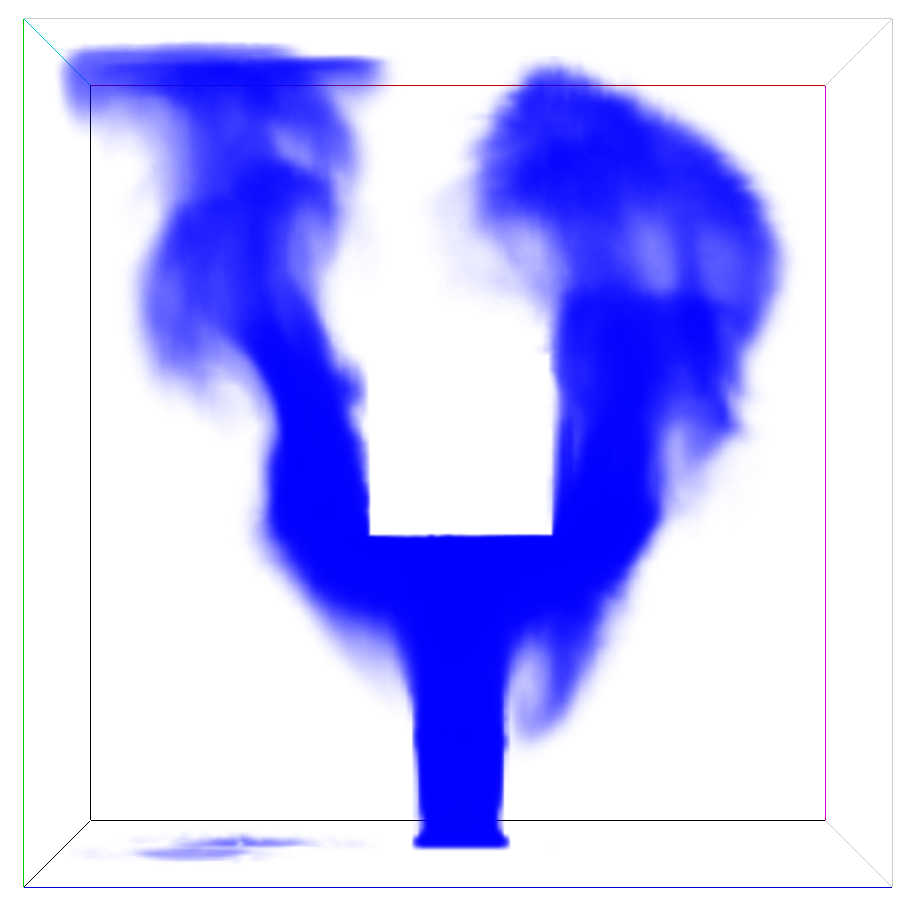
\includegraphics[width=65mm]{images/n128_dev2_f99_obstacle.png}
\subcaption{分割数2}
\end{minipage}

\begin{minipage}[b]{0.45\linewidth}
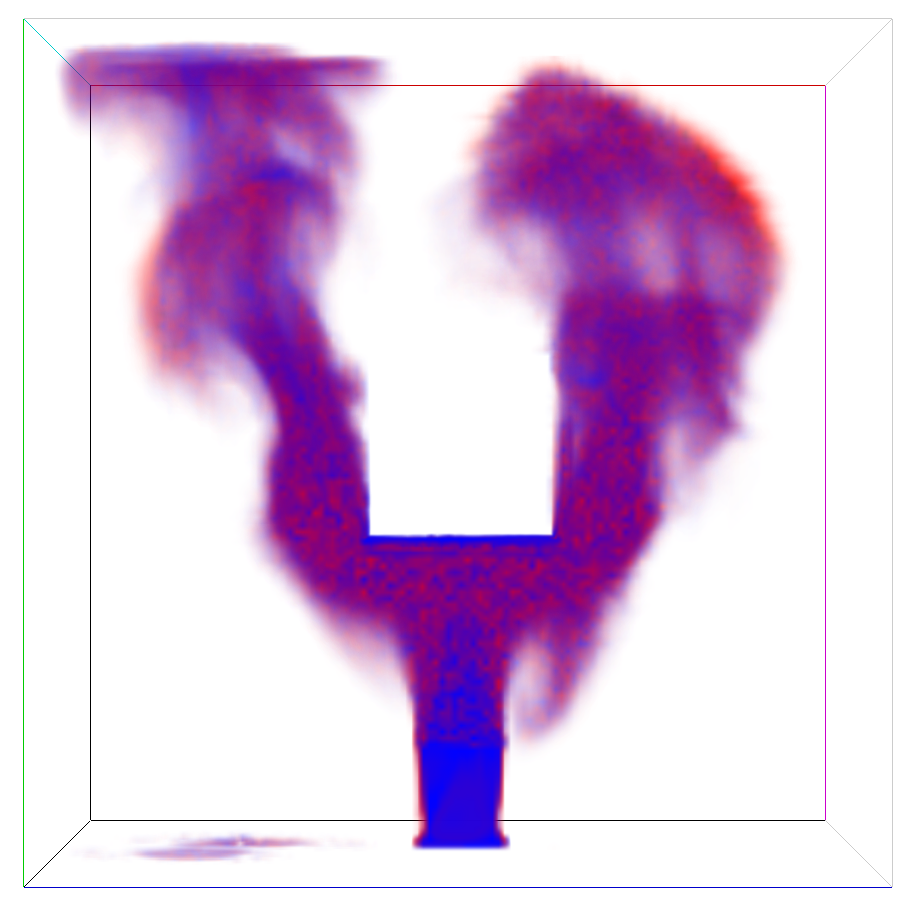
\includegraphics[width=65mm]{images/n128_dev2_f99_obstacle_color.png}
\subcaption{分割数2,誤差による色付け}
\end{minipage}
\end{tabular}
\end{figure}

\begin{figure}[htbp]
\caption{$解像度128^3,障害物あり,101フレーム目$}
\label{fig:n128_f100_obstacle}
\centering
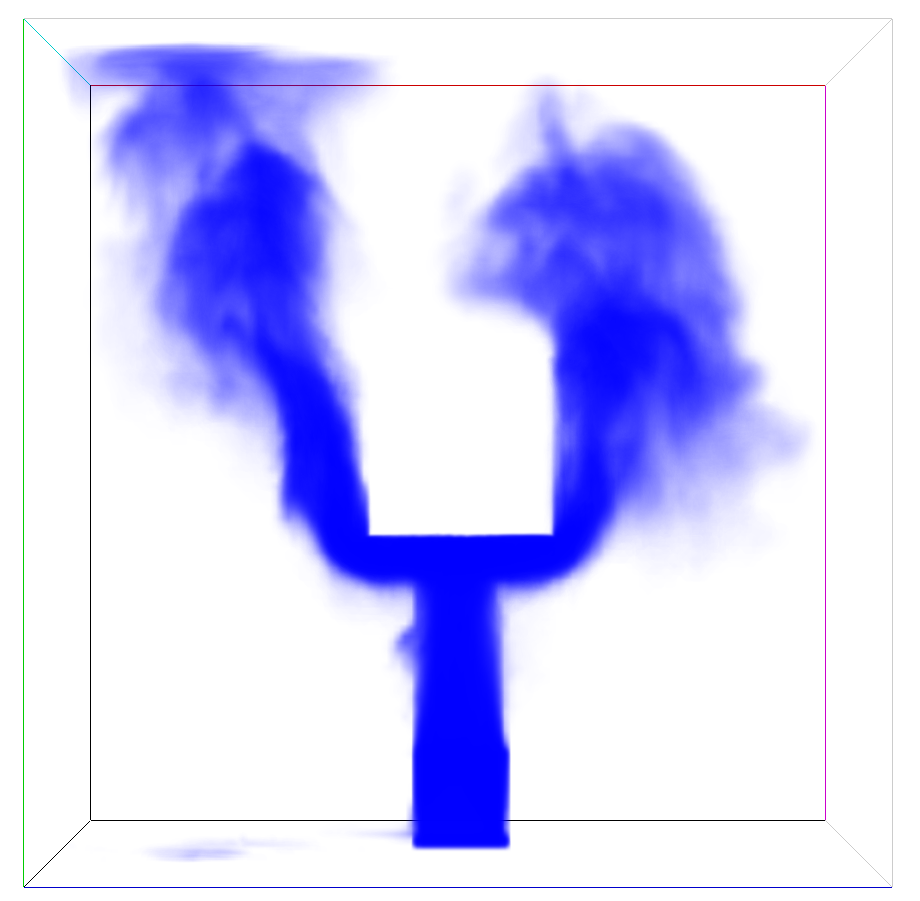
\includegraphics[width=65mm]{images/n128_origin_f100_obstacle.png}
\subcaption{gruound truth}

\begin{tabular}{cc}
\begin{minipage}[b]{0.45\linewidth}
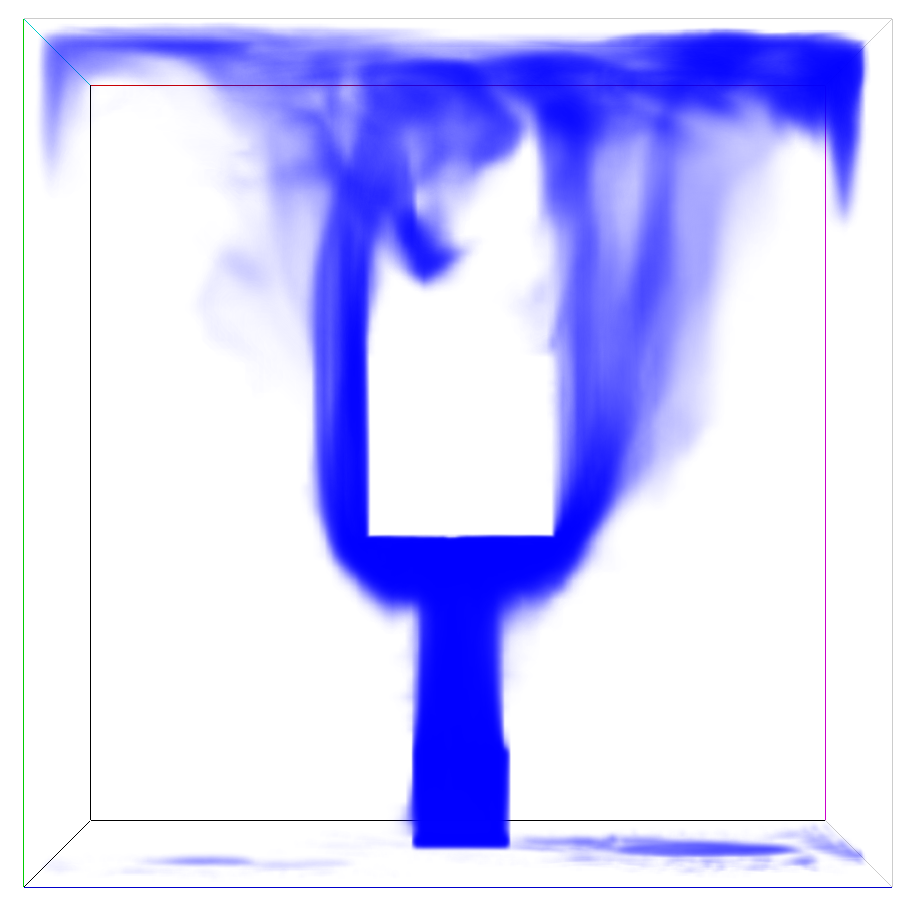
\includegraphics[width=65mm]{images/n128_dev1_f100_obstacle.png}
\subcaption{分割数1}
\end{minipage}

\begin{minipage}[b]{0.45\linewidth}
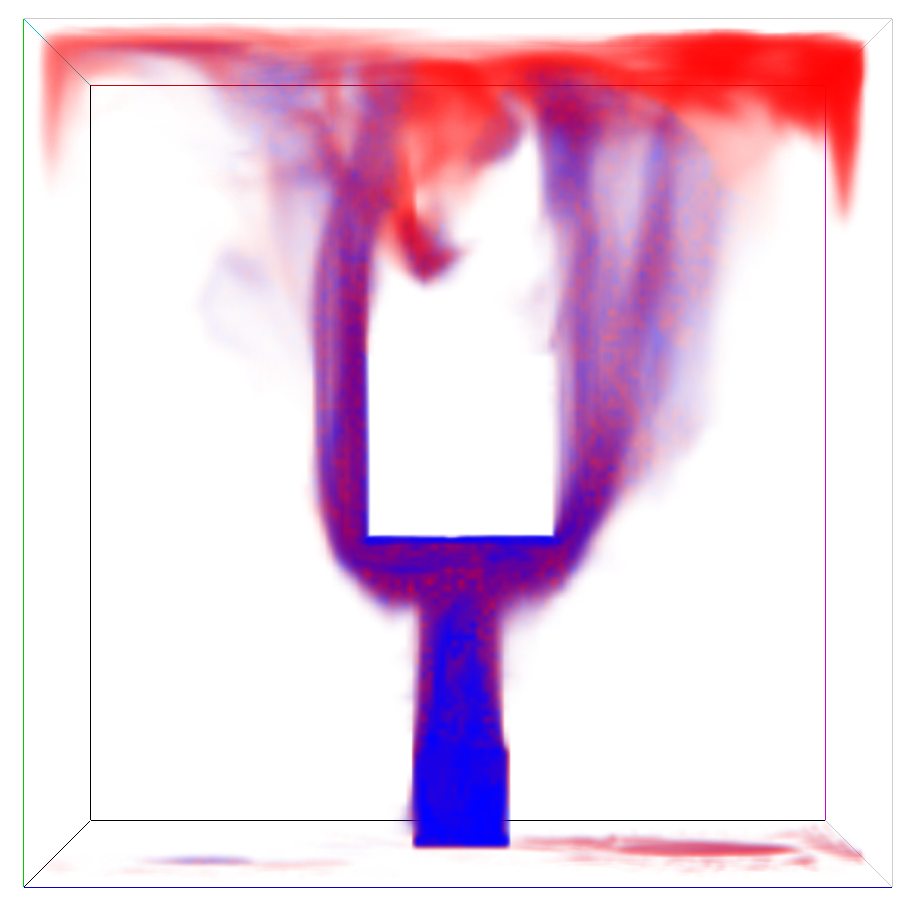
\includegraphics[width=65mm]{images/n128_dev1_f100_obstacle_color.png}
\subcaption{分割数1,誤差による色付け}
\end{minipage}
\\
\begin{minipage}[b]{0.45\linewidth}
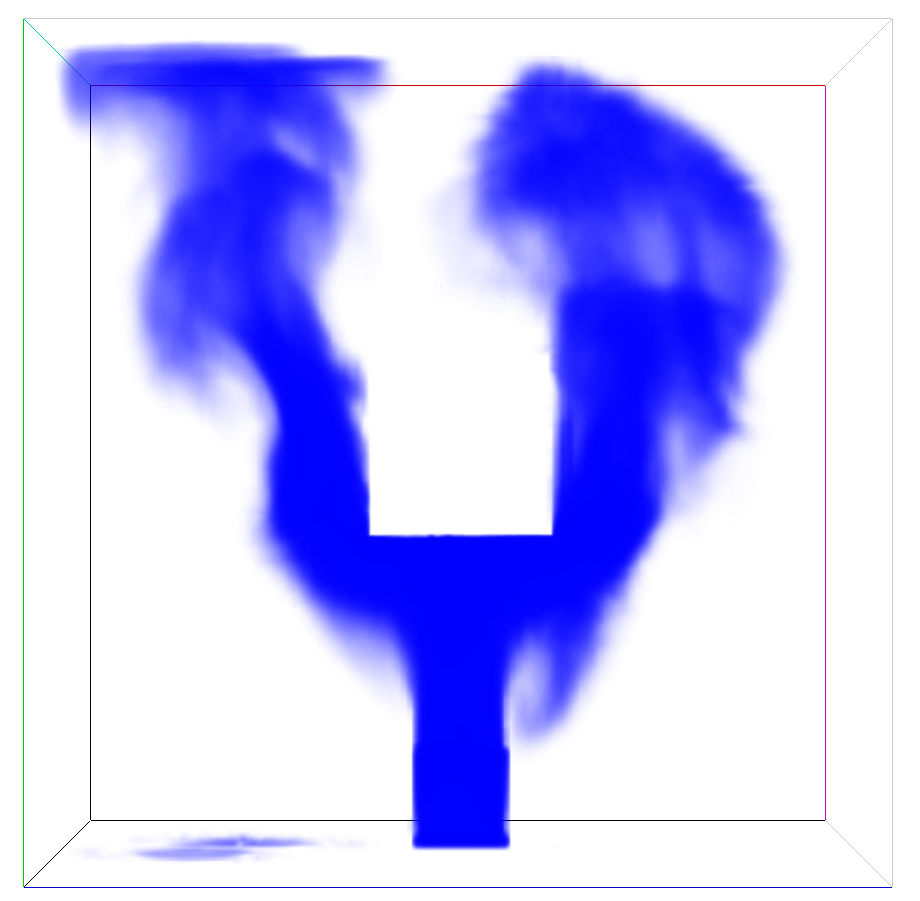
\includegraphics[width=65mm]{images/n128_dev2_f100_obstacle.png}
\subcaption{分割数2}
\end{minipage}

\begin{minipage}[b]{0.45\linewidth}
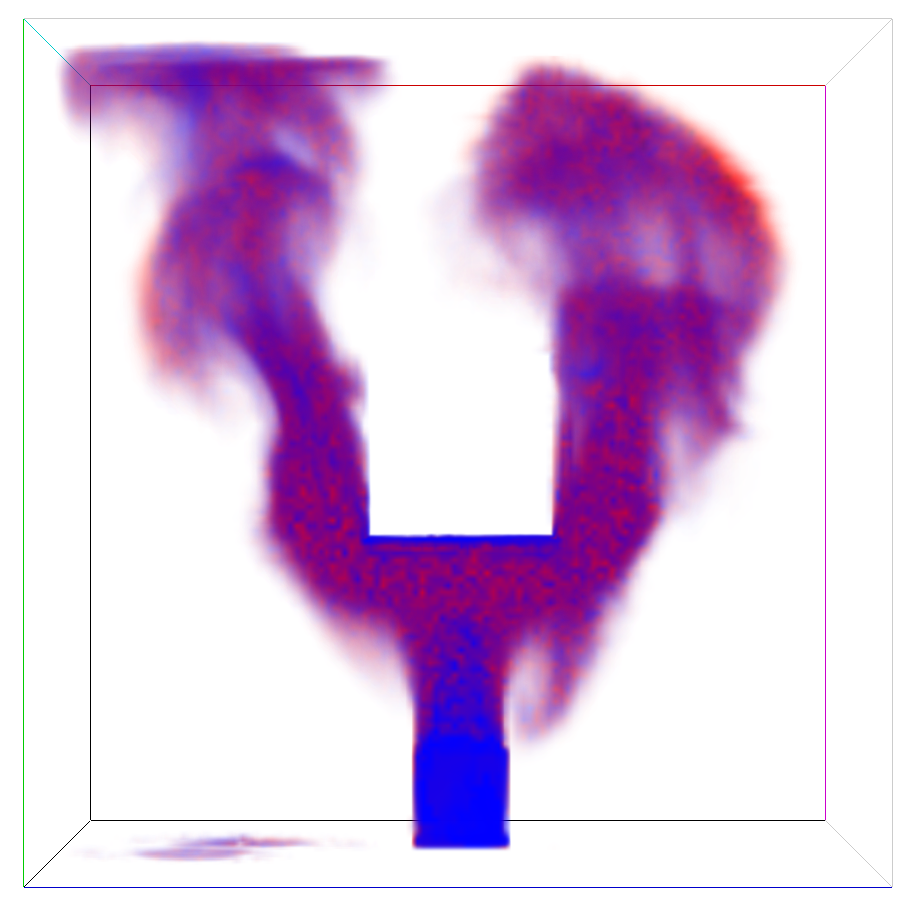
\includegraphics[width=65mm]{images/n128_dev2_f100_obstacle_color.png}
\subcaption{分割数2,誤差による色付け}
\end{minipage}
\end{tabular}
\end{figure}
%\begin{figure}[htbp]
%\caption{$解像度128^3,100フレーム目$}
%\label{fig:n128_f100}
%\centering
%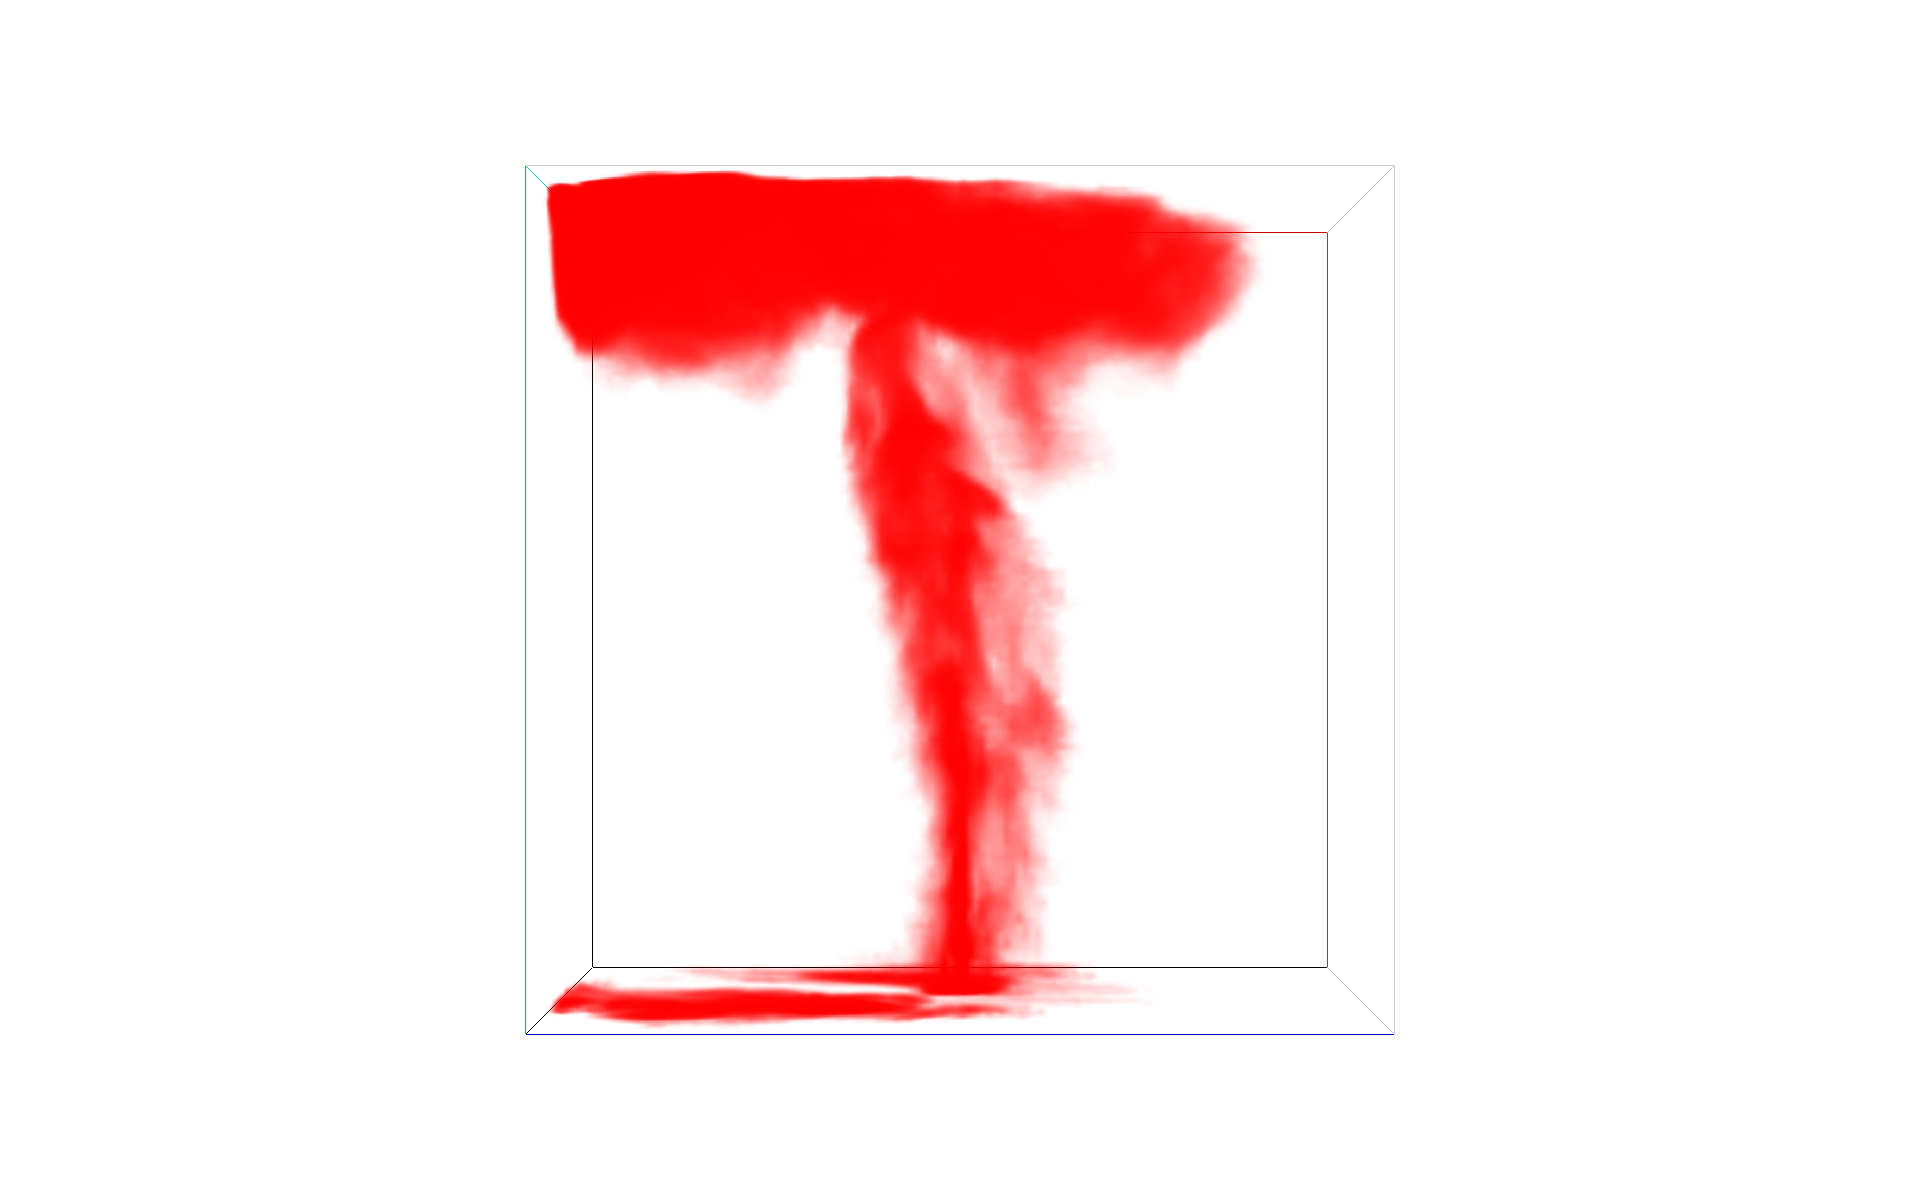
\includegraphics[width=100mm]{images/n128_f100_truth.png}
%\subcaption{gruound truth}
%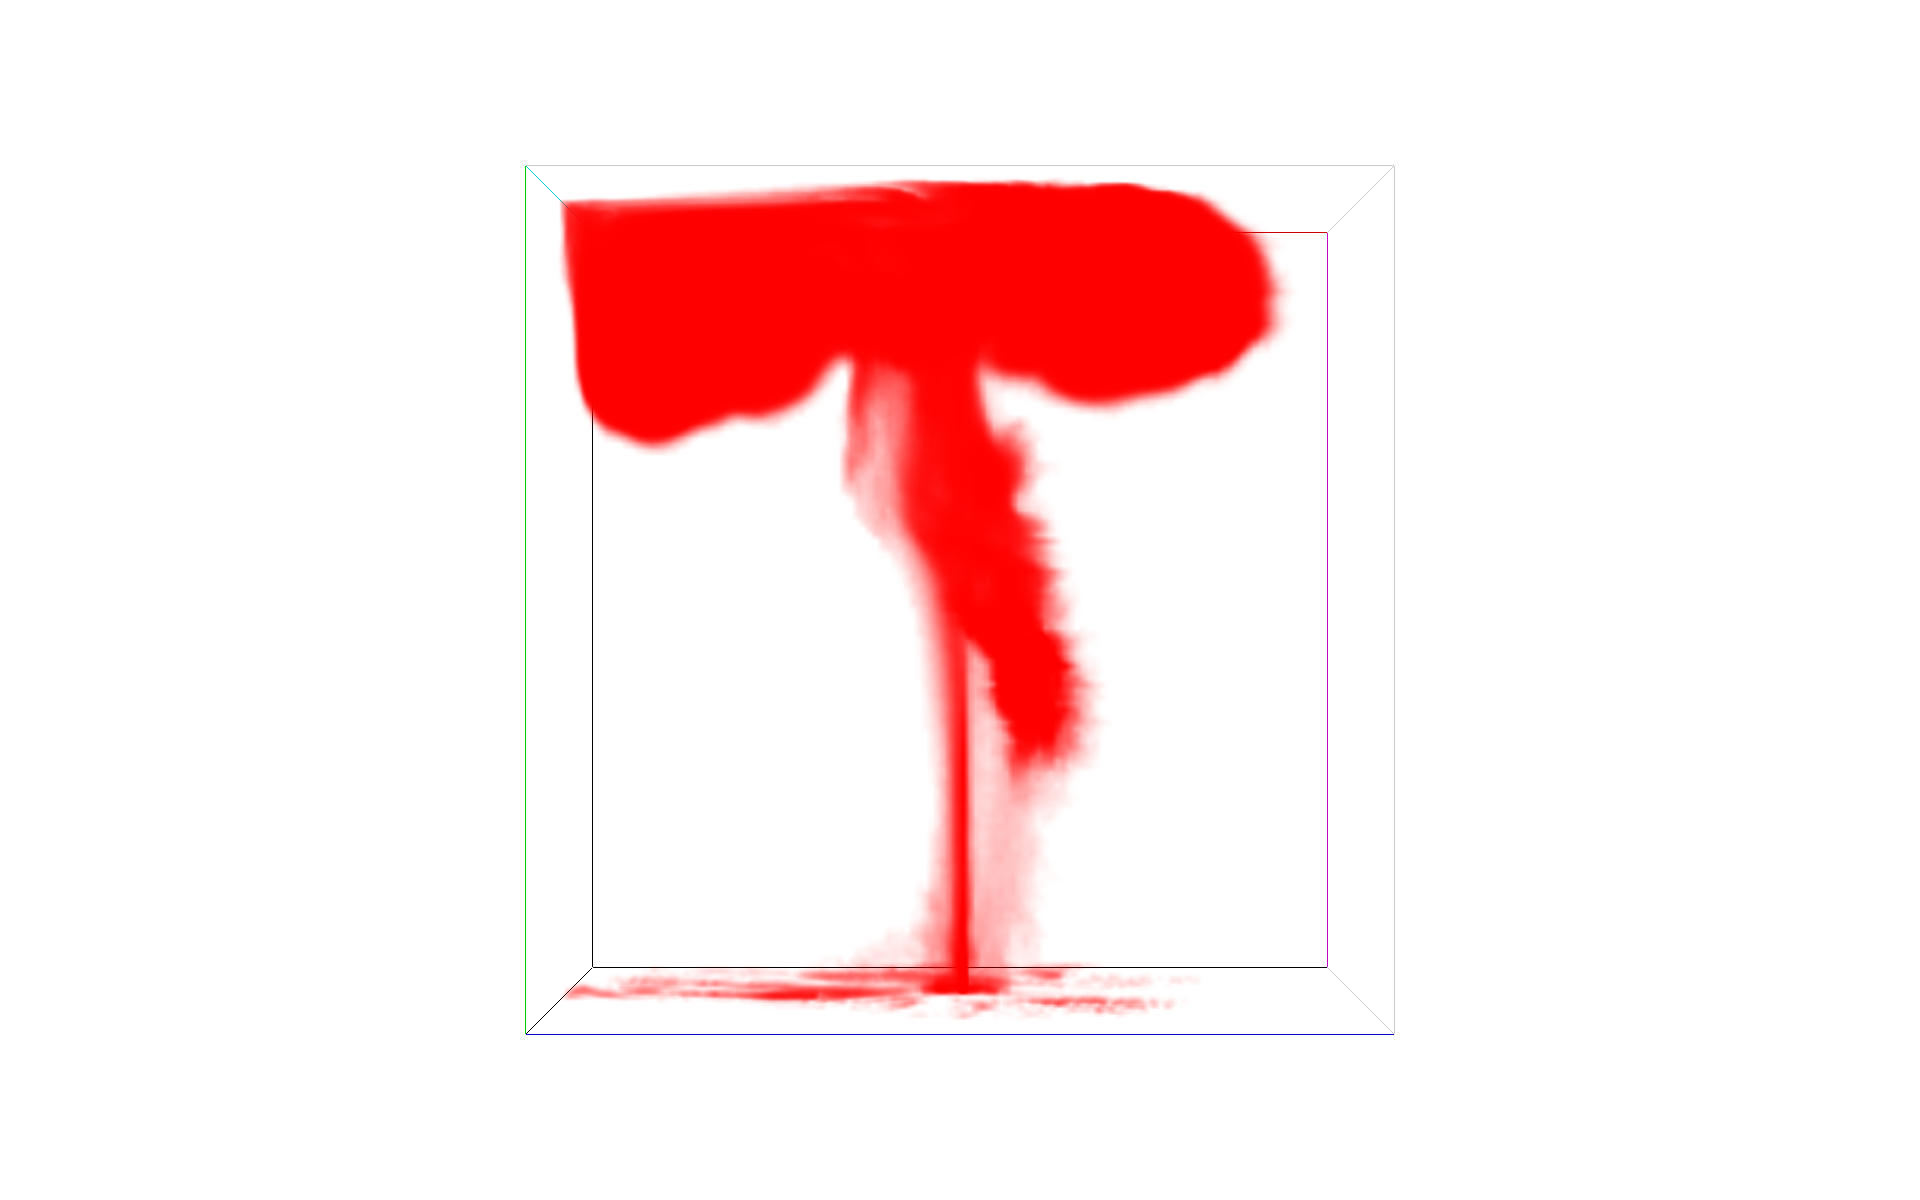
\includegraphics[width=100mm]{images/n128_f100_dev1.png}
%\subcaption{分割数1}
%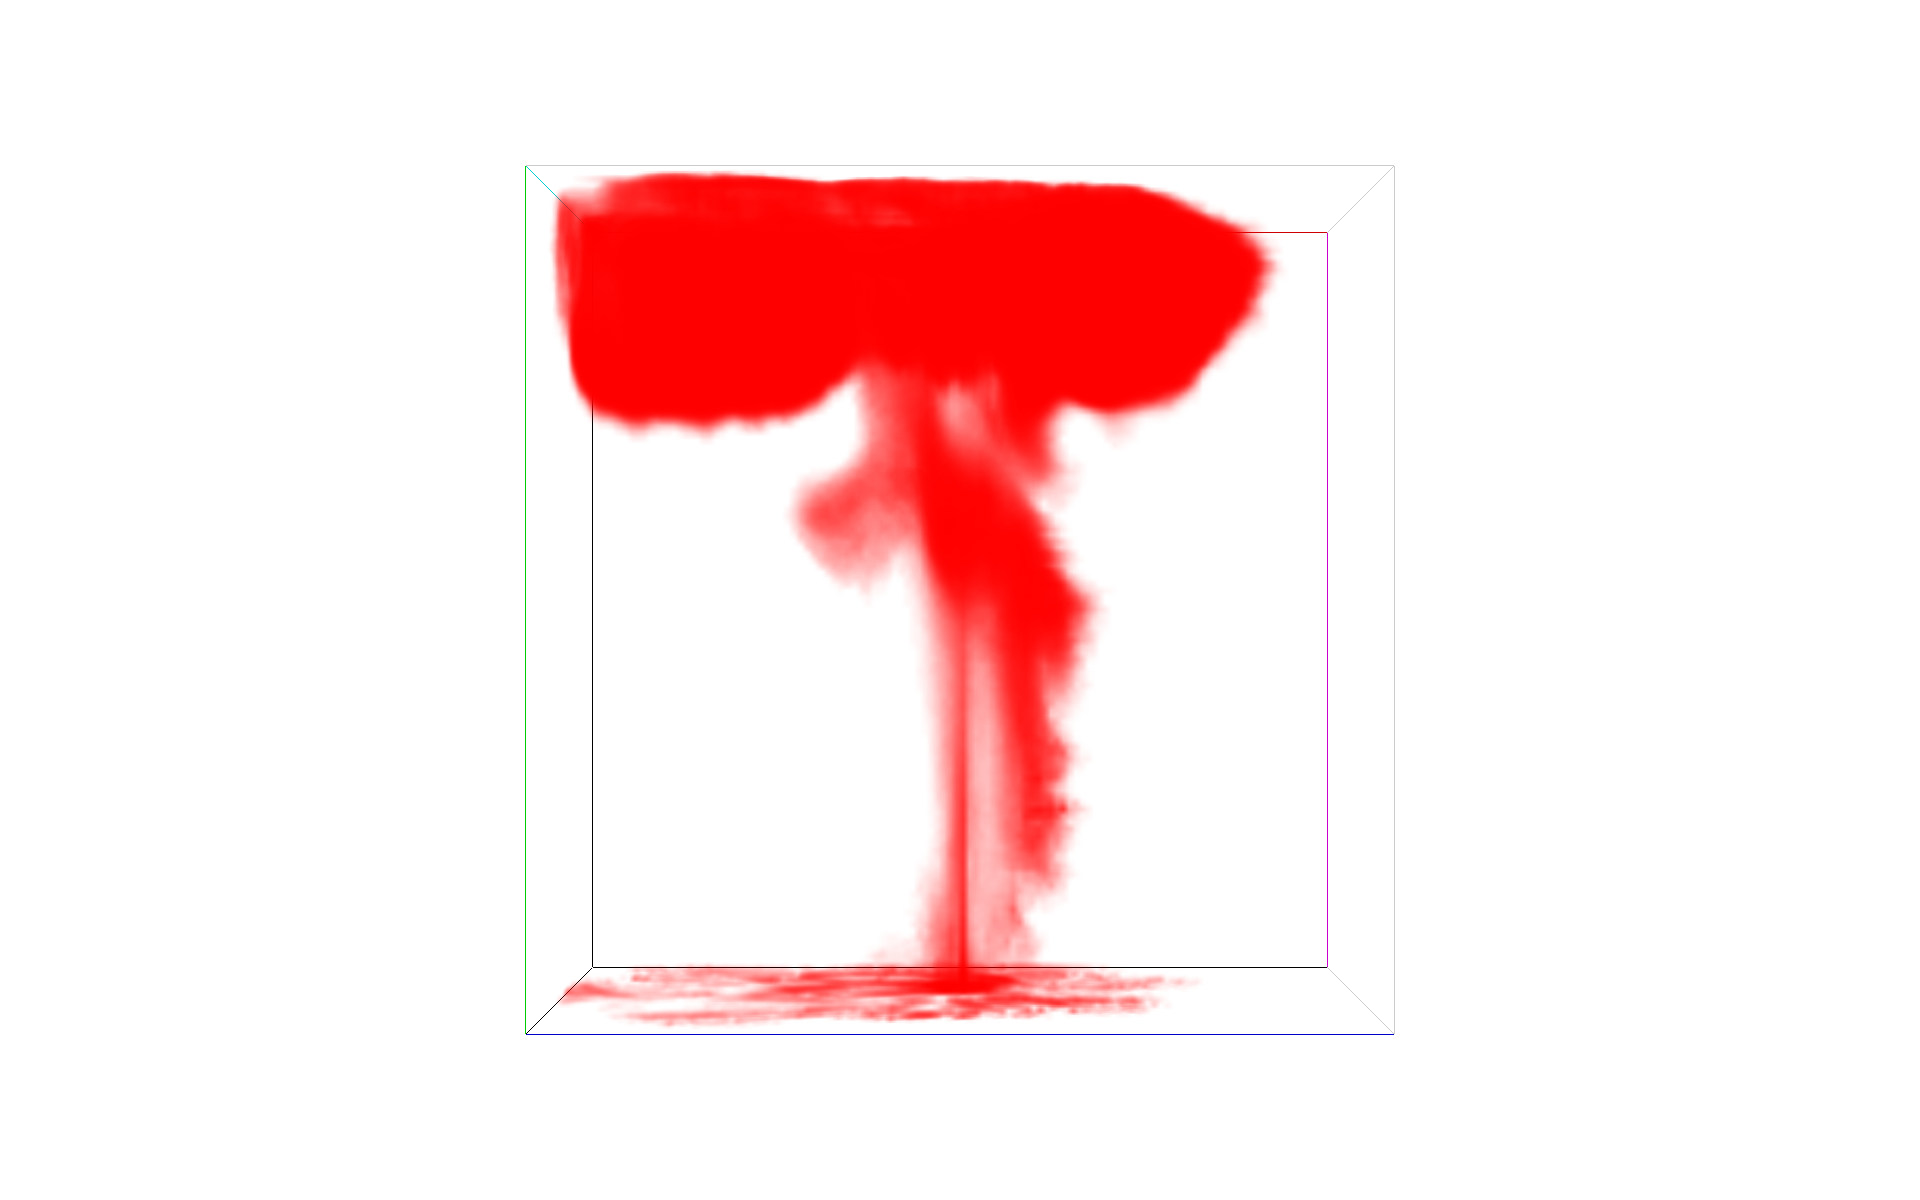
\includegraphics[width=100mm]{images/n128_f100_dev2.png}
%\subcaption{分割数2}
%\end{figure}



%\begin{figure}[htbp]
%\caption{$解像度128^3,180フレーム目$}
%\label{fig:n128_f100}
%\centering
%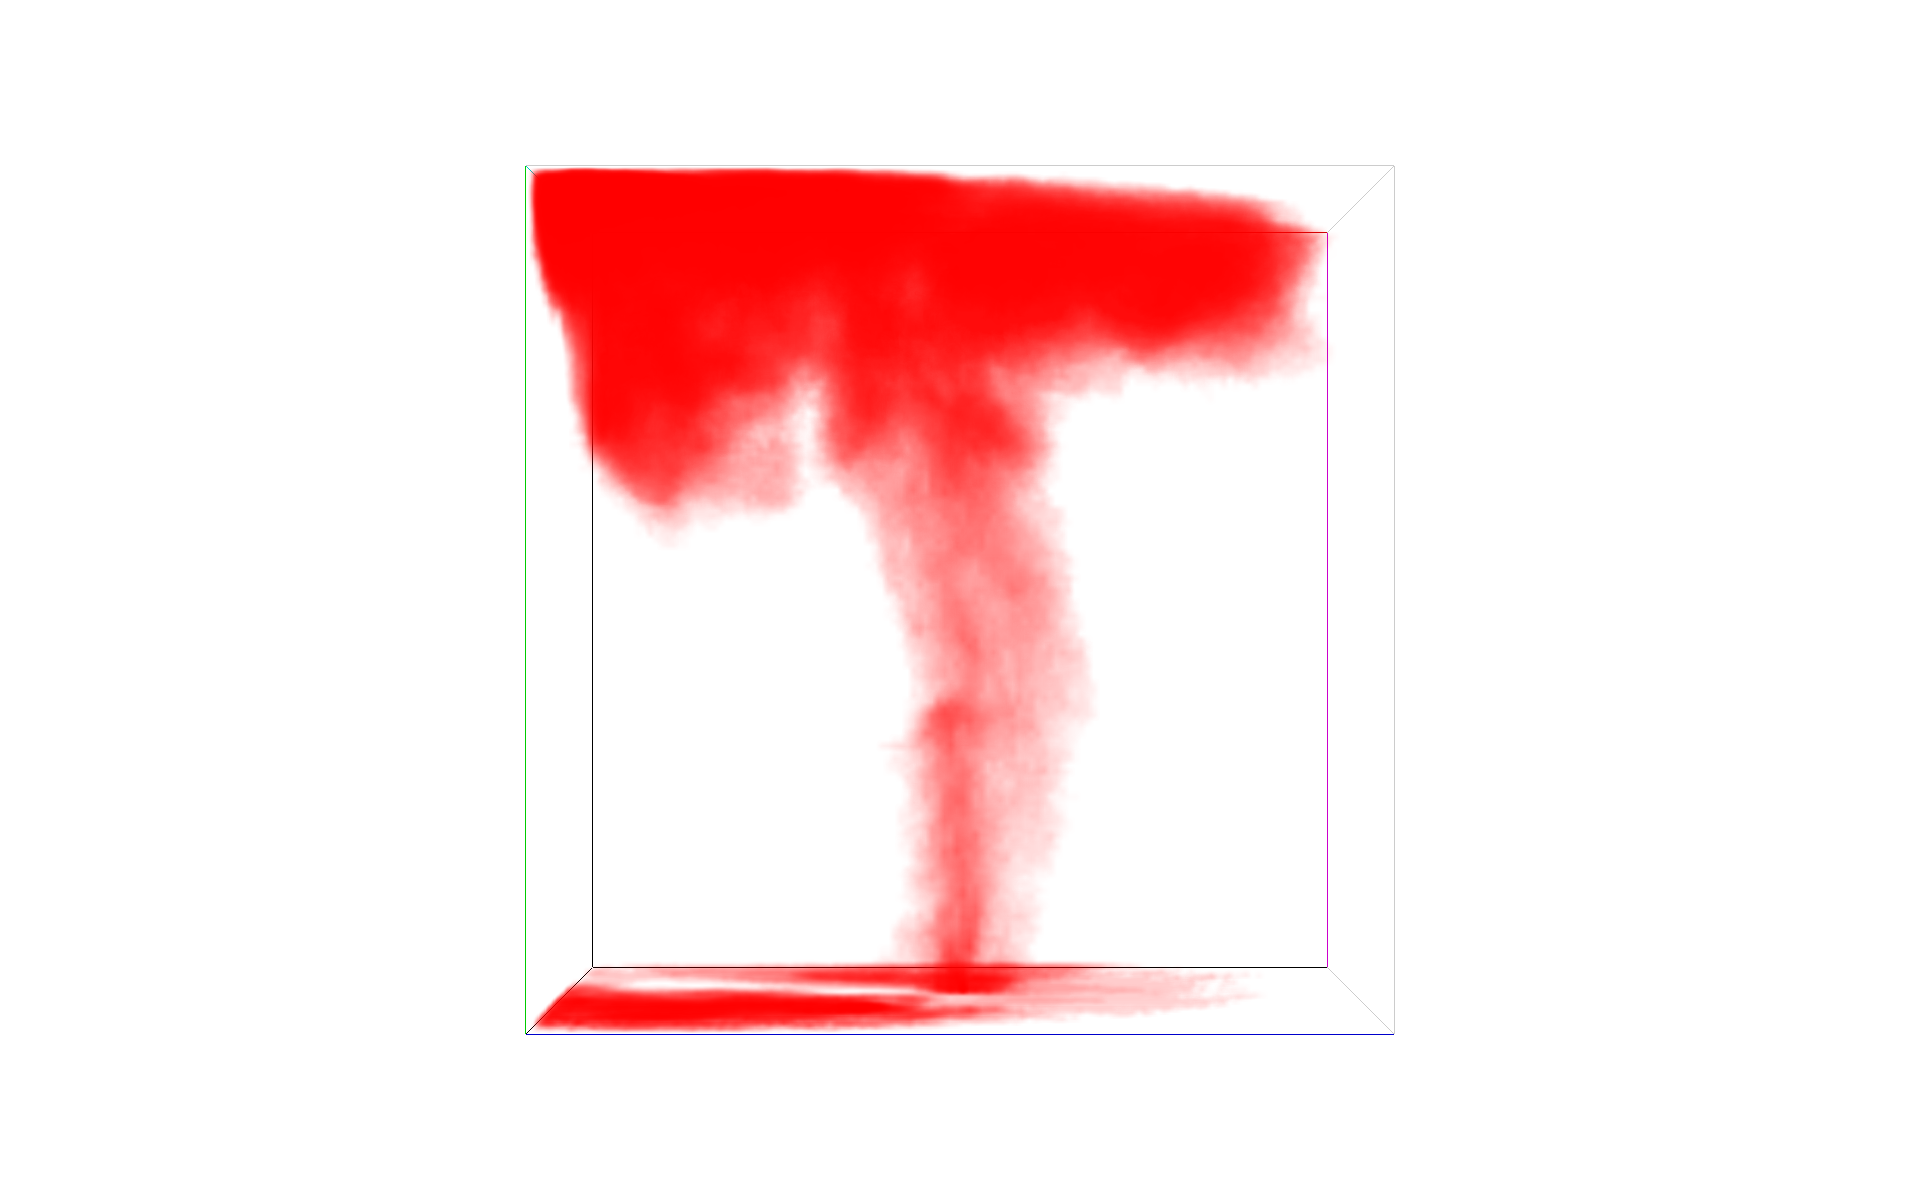
\includegraphics[width=100mm]{images/n128_f180_truth.png}
%\subcaption{gruound truth}
%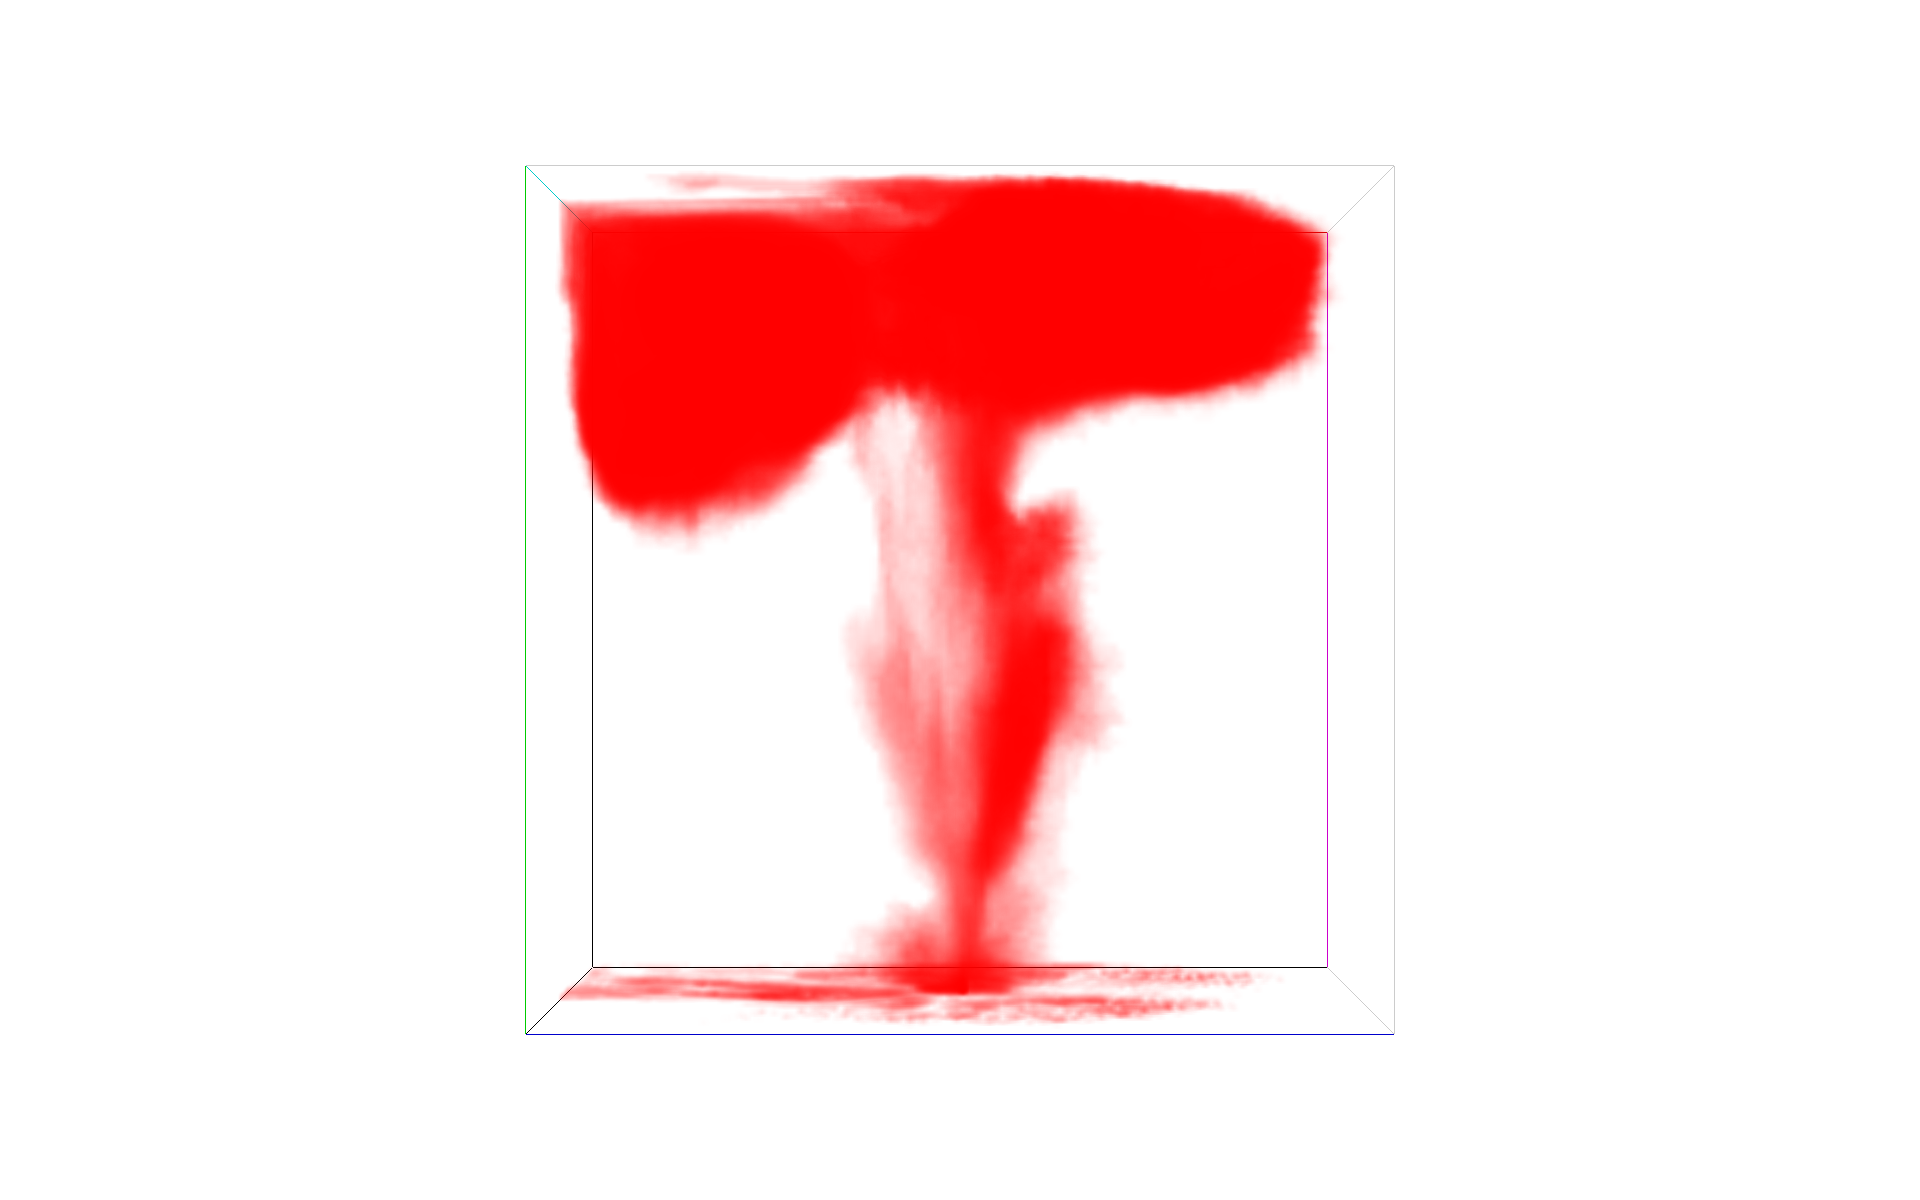
\includegraphics[width=100mm]{images/n128_f180_dev1.png}
%\subcaption{分割数1}
%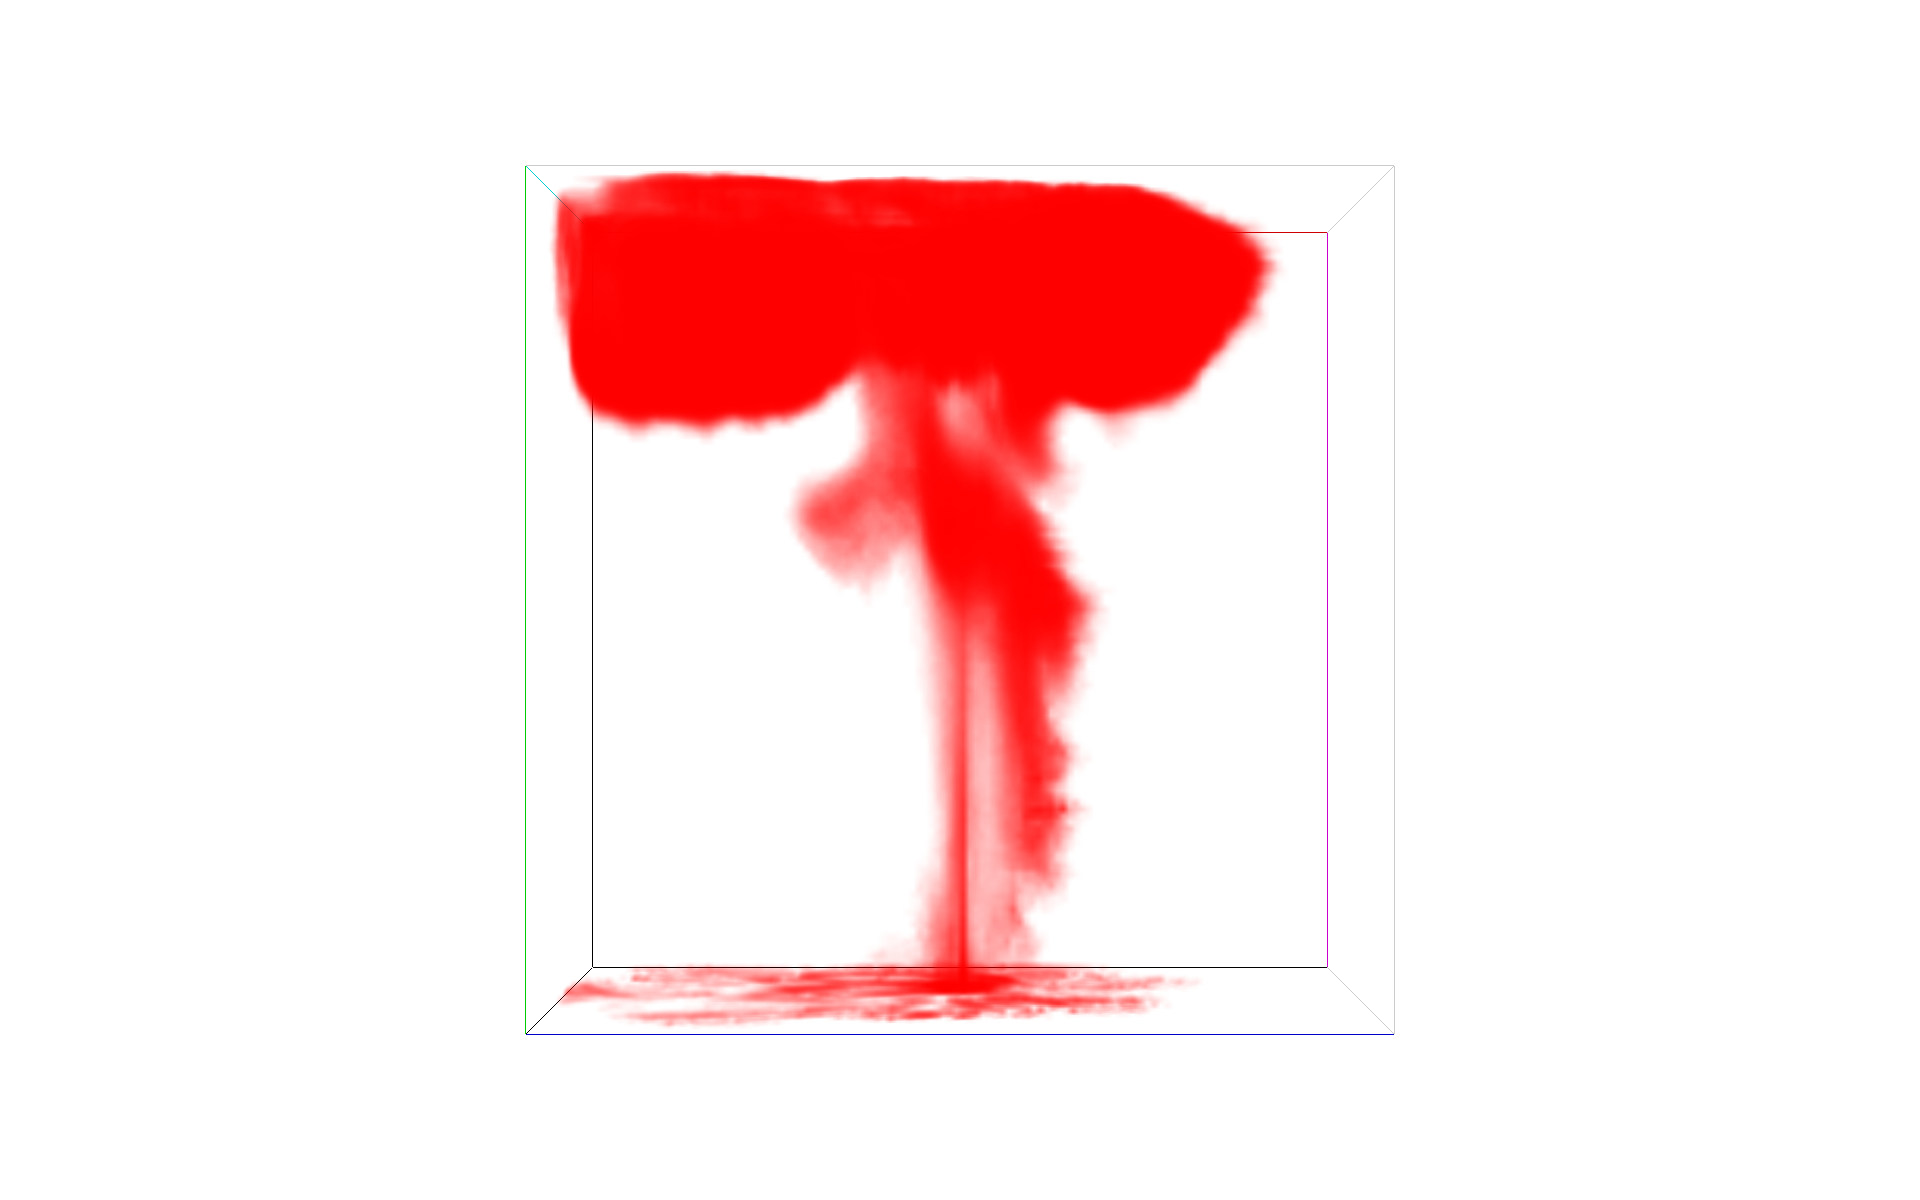
\includegraphics[width=100mm]{images/n128_f100_dev2.png}
%\subcaption{分割数2}
%\end{figure}
\section{考察}

%解像度$128^3$における計算時間が,分割なしと分割数2で劇的に向上しているのは,スナップショット行列の空間計算量が計算機のメモリを超えてしまい,メモリ領域外アクセスが発生してしまったためだと考えられる.

%分割なしと比べて精度が向上している点については,分割なしでは抽出されなかったモードを抽出することができていることによって,シミュレーション後半の流れを詳細にシミュレーションできていると考えられる.特異値分解を用いた次元削減はの条件数は,行列を構成する列ベクトル同士の相関が強いほど悪くなることが知られている.本実験のシミュレーションの開始直後においては,タイムステップごとの流速や圧力の変化が大きくスナップショット間の相関関係が弱い.一方でシミュレーション終了付近においては,タイムステップごとの流速や圧力の変化が大きくスナップショット間の相関関係が強い.スナップショットの分割によって各基底の最大特異値が小さくなることによって,分割前と比較してシミュレーション後半に対応する特異値に関する条件数が改善され,詳細にシミュレーションできていると考えられる.


部分空間法において,基底による近似誤差が常に発生する.特に急激な流れの変動があった場合,元のデータを十分に近似するには多数のモードを用いる必要があり,用いる基底が固定されていると元の流れを再現できず,誤差が発生する.これに対して,基底を切り替えたとき精度が誤差が大きく減少する.これはスナップショットの範囲を限定した基底を用いることで,流れの特徴をよりよく再現することができたためと考えられる.特に障害物ありのシミュレーションにおいて,障害物との衝突により流れが急速に変化するため,基底を切り替えたことでより良い再現ができたと考えられる.一方で,速度の局所的な精度向上は,密度分布にはすぐに反映されない.これは密度は流速に従って逐次的に変化するためである.

分割後の累積寄与率は分割前よりも大きいのに対して,シミュレーションの相対誤差は分割後の方が大きい場合がある.これは,累積寄与率は直接シミュレーションの誤差を測る指標ではないためである.特に抽出するモードが細部の流れを再現できない場合に誤差が大きくなる可能性がある.


\chapter{終わりに}
流体シミュレーションにおける部分空間法の前処理にかかる計算時間に対し,スナップショットを分割することによって高速化する手法を提案した.特に基底計算については分割数に応じた高速化を達成し,前処理全体の高速化を達成した.スナップショット分割によるシミュレーションの結果の精度に関しては,既存手法と提案手法の間の相対誤差を計算し,煙のアニメーションの誤差について計測を行った.

%今後の研究として,最適なスナップショット分割を決定する手法が考えられる.
今後の研究として,GPUを用いた大規模高速計算の併用などを用いた高速化が挙げられる.
部分空間法の高速化について,シミュレーション結果を離散コサイン変換(DCT)を用いて圧縮する手法\cite{subspaceDCT}が研究されている.この手法はシミュレーション結果を離散コサイン変換を用いて圧縮し,必要に応じて展開することで,GPUを用いた大規模高速計算を改善する手法である.提案した手法を組み込むことで,より高速な基底計算を達成できるかについて検討する.


%謝辞
\syaji
\par
本研究を進めるにあたり,大変多くのご指導,ご助言を頂いた
中央大学理工学部情報工学科の森口昌樹 准教授に深く感謝いたします.3年間に渡り,研究の進め方や,開発方法について大変多くのご指導をいただきました.また,多大なるご助言,ご協力を頂いた形状情報処理研究室の皆様には大変お世話になりました.心から感謝いたします.
最後に,研究生活を支えてくれた家族にも感謝いたします.
%参考文献
\begin{thebibliography}{99}
\addcontentsline{toc}{chapter}{参考文献}
\bibitem{subspaceDCT}
A. D. Jones, P. Sen, and T. Kim. Compressing fluid subspaces. \textit{Proceedings of the ACM SIGGRAPH/Eurographics Symposium on Computer Animation}, 77--84, 2016.

\bibitem{Chorin}
A. J. Chorin. Numerical Solution of the Navier-Stokes Equations. \textit{Mathematics of Computation}, 22(104): 745--762, 1968.

\bibitem{projection_base}
A. Treuille, A. Lewis, and Z. Popovic. Model Reduction for Real-time Fluids. \textit{ACM Transactions on Graphics},25(3):826--834, 2006.

\bibitem{APIC}
C. Jiang, C. Schroeder, A. Selle, J. Teran, A. Stomakhin, The affine particle-in-cell method. \textit{ACM Transactions on Graphics},34(4):51:1 -- 51:10, 2015.

\bibitem{MAC}
F. H. Harlow and J. E. Welch. Numerical calculation of time-dependent viscous incompressible flow of fluid with a free surface. \textit{Physics of Fluids}, 8(12): 2182--2189, 1965.

\bibitem{stam}
J. Stam. Stable Fluids. In \textit{SIGGRAPH 99 Conference Proceedings, Annual Conference Series}, pages 121--128, 1999.

\bibitem{FLIP}
J. U. Brackbill. D. B. KotheH.M.Ruppel. Flip: A low-dissipation, particle-in-cell method for fluid flow, \textit{Computer Physics Communications}, 48(1),25--38, 1988.

\bibitem{fedkiw}
R. Fedkiew, J. stam, H. Jensen. Visual simulation of smoke. In \textit{Proceedings of SIGGRAPH 01}, 15--22, 2001.

\bibitem{subspace}
T. Kim, J. Delaney. Subspace Fluid Re-Simulation. \textit{ACM Transactions on Graphics},32(4): 62:1--62:9, 2013.

\bibitem{EOL}
Y. Teng, David I.W. Levin, T. Kim.Eulerian Solid-Fluid Coupling. \textit{ACM Transactions on Graphics}, 35, (6):  200:1--200:8, 2016.

\end{thebibliography}

\end{document}